\ifx\XeTeXversion\undefined\pdfoutput=1\fi % arXiv: pdflatex; local builds with tectonic (XeTeX) skip it
\documentclass[10pt,a4paper]{article}
\usepackage[T1]{fontenc}
\usepackage[utf8]{inputenc}
\usepackage{lmodern}
\usepackage[margin=2.2cm]{geometry}
\usepackage{amsmath,amssymb}
\usepackage{booktabs,multirow,longtable,array,tabularx}
\usepackage{graphicx}
\usepackage[table]{xcolor}
\usepackage{microtype}
\usepackage{caption}
\usepackage[hidelinks]{hyperref}
\usepackage{xspace}
\usepackage[section]{placeins}
\renewcommand{\topfraction}{0.9}\renewcommand{\bottomfraction}{0.8}\renewcommand{\textfraction}{0.07}\renewcommand{\floatpagefraction}{0.8}\setcounter{totalnumber}{6}\setcounter{topnumber}{4}

% ---------------------------------------------------------------- numbers
% Every number in the prose comes from numbers.tex (generated by analysis/mktex.py);
% \nm{key} prints it, and a missing key prints a visible marker instead of a silent gap.
\newcommand{\defnum}[2]{\expandafter\def\csname num@#1\endcsname{#2}}
\newcommand{\nm}[1]{\ifcsname num@#1\endcsname\csname num@#1\endcsname\else\textbf{\textcolor{red}{??#1??}}\fi}
% Generated by paper/analysis/mktex.py. Do not edit by hand.
\defnum{agent.repos.eff}{6.8}
\defnum{agent.repos.max}{376}
\defnum{agent.repos.min}{21}
\defnum{agent.repos.top5}{80}
\defnum{beir.cut.nfcorpus}{92}
\defnum{beir.cut.scifact}{91}
\defnum{beirset.amd.NumKong.bf16}{9}
\defnum{beirset.amd.NumKong.f16}{10}
\defnum{beirset.amd.NumKong.f32}{11}
\defnum{beirset.arm.NumKong.bf16}{16}
\defnum{beirset.arm.NumKong.f16}{16}
\defnum{beirset.arm.NumKong.f32}{16}
\defnum{beirset.arm.PyTorch.bf16}{11}
\defnum{beirset.epyc.NumPy.f32}{1}
\defnum{beirset.intel.NumKong.bf16}{20}
\defnum{beirset.intel.NumKong.f16}{20}
\defnum{beirset.intel.NumKong.f32}{20}
\defnum{beirset.intel.PyTorch.bf16}{12}
\defnum{beirset.intel.PyTorch.f32}{20}
\defnum{beirset.m3max.NumKong.bf16}{12}
\defnum{beirset.m3max.NumKong.f16}{12}
\defnum{beirset.m3max.NumKong.f32}{11}
\defnum{beirset.m3max.PyTorch.f32}{2}
\defnum{best.parked.agent-ho.any.max}{1.40}
\defnum{best.parked.agent-ho.any.min}{0.61}
\defnum{best.parked.agent-ho.any.nointel.max}{1.40}
\defnum{best.parked.agent-ho.any.nointel.min}{0.71}
\defnum{best.parked.agent-ho.f32.max}{1.40}
\defnum{best.parked.agent-ho.f32.min}{0.61}
\defnum{best.parked.agent-ho.f32.nointel.max}{1.40}
\defnum{best.parked.agent-ho.f32.nointel.min}{0.71}
\defnum{best.parked.amd.agent-ho.any}{1.40}
\defnum{best.parked.amd.agent-ho.any.lib}{NumPy}
\defnum{best.parked.amd.agent-ho.f32}{1.40}
\defnum{best.parked.amd.agent-ho.f32.lib}{NumPy}
\defnum{best.parked.amd.beir.any}{1.18}
\defnum{best.parked.amd.beir.any.lib}{PyTorch (bf16)}
\defnum{best.parked.amd.beir.f32}{1.27}
\defnum{best.parked.amd.beir.f32.lib}{PyTorch}
\defnum{best.parked.amd.gcsn-ho.any}{1.34}
\defnum{best.parked.amd.gcsn-ho.any.lib}{NumPy}
\defnum{best.parked.amd.gcsn-ho.f32}{1.34}
\defnum{best.parked.amd.gcsn-ho.f32.lib}{NumPy}
\defnum{best.parked.arm.agent-ho.any}{0.94}
\defnum{best.parked.arm.agent-ho.any.lib}{NumPy}
\defnum{best.parked.arm.agent-ho.f32}{0.94}
\defnum{best.parked.arm.agent-ho.f32.lib}{NumPy}
\defnum{best.parked.arm.beir.any}{1.28}
\defnum{best.parked.arm.beir.any.lib}{NumPy}
\defnum{best.parked.arm.beir.f32}{1.28}
\defnum{best.parked.arm.beir.f32.lib}{NumPy}
\defnum{best.parked.arm.gcsn-ho.any}{0.82}
\defnum{best.parked.arm.gcsn-ho.any.lib}{NumPy}
\defnum{best.parked.arm.gcsn-ho.f32}{0.82}
\defnum{best.parked.arm.gcsn-ho.f32.lib}{NumPy}
\defnum{best.parked.beir.any.max}{1.28}
\defnum{best.parked.beir.any.min}{0.79}
\defnum{best.parked.beir.any.nointel.max}{1.28}
\defnum{best.parked.beir.any.nointel.min}{1.18}
\defnum{best.parked.beir.f32.max}{1.28}
\defnum{best.parked.beir.f32.min}{0.79}
\defnum{best.parked.beir.f32.nointel.max}{1.28}
\defnum{best.parked.beir.f32.nointel.min}{1.27}
\defnum{best.parked.epyc.agent-ho.any}{0.71}
\defnum{best.parked.epyc.agent-ho.any.lib}{NumPy}
\defnum{best.parked.epyc.agent-ho.f32}{0.71}
\defnum{best.parked.epyc.agent-ho.f32.lib}{NumPy}
\defnum{best.parked.epyc.gcsn-ho.any}{0.69}
\defnum{best.parked.epyc.gcsn-ho.any.lib}{NumPy}
\defnum{best.parked.epyc.gcsn-ho.f32}{0.69}
\defnum{best.parked.epyc.gcsn-ho.f32.lib}{NumPy}
\defnum{best.parked.gcsn-ho.any.max}{1.34}
\defnum{best.parked.gcsn-ho.any.min}{0.50}
\defnum{best.parked.gcsn-ho.any.nointel.max}{1.34}
\defnum{best.parked.gcsn-ho.any.nointel.min}{0.69}
\defnum{best.parked.gcsn-ho.f32.max}{1.34}
\defnum{best.parked.gcsn-ho.f32.min}{0.50}
\defnum{best.parked.gcsn-ho.f32.nointel.max}{1.34}
\defnum{best.parked.gcsn-ho.f32.nointel.min}{0.69}
\defnum{best.parked.intel.agent-ho.any}{0.61}
\defnum{best.parked.intel.agent-ho.any.lib}{NumPy}
\defnum{best.parked.intel.agent-ho.f32}{0.61}
\defnum{best.parked.intel.agent-ho.f32.lib}{NumPy}
\defnum{best.parked.intel.beir.any}{0.79}
\defnum{best.parked.intel.beir.any.lib}{NumPy}
\defnum{best.parked.intel.beir.f32}{0.79}
\defnum{best.parked.intel.beir.f32.lib}{NumPy}
\defnum{best.parked.intel.gcsn-ho.any}{0.50}
\defnum{best.parked.intel.gcsn-ho.any.lib}{NumPy}
\defnum{best.parked.intel.gcsn-ho.f32}{0.50}
\defnum{best.parked.intel.gcsn-ho.f32.lib}{NumPy}
\defnum{best.parked.m3max.agent-ho.any}{0.92}
\defnum{best.parked.m3max.agent-ho.any.lib}{NumPy}
\defnum{best.parked.m3max.agent-ho.f32}{0.92}
\defnum{best.parked.m3max.agent-ho.f32.lib}{NumPy}
\defnum{best.parked.m3max.gcsn-ho.any}{0.74}
\defnum{best.parked.m3max.gcsn-ho.any.lib}{NumPy}
\defnum{best.parked.m3max.gcsn-ho.f32}{0.74}
\defnum{best.parked.m3max.gcsn-ho.f32.lib}{NumPy}
\defnum{best.single.agent-ho.any.max}{1.14}
\defnum{best.single.agent-ho.any.min}{0.24}
\defnum{best.single.agent-ho.any.nointel.max}{1.12}
\defnum{best.single.agent-ho.any.nointel.min}{0.24}
\defnum{best.single.agent-ho.f32.max}{1.14}
\defnum{best.single.agent-ho.f32.min}{0.24}
\defnum{best.single.agent-ho.f32.nointel.max}{1.12}
\defnum{best.single.agent-ho.f32.nointel.min}{0.24}
\defnum{best.single.amd.agent-ho.any}{1.08}
\defnum{best.single.amd.agent-ho.any.lib}{NumPy}
\defnum{best.single.amd.agent-ho.f32}{1.08}
\defnum{best.single.amd.agent-ho.f32.lib}{NumPy}
\defnum{best.single.amd.beir.any}{0.77}
\defnum{best.single.amd.beir.any.lib}{NumPy}
\defnum{best.single.amd.beir.f32}{0.77}
\defnum{best.single.amd.beir.f32.lib}{NumPy}
\defnum{best.single.amd.gcsn-ho.any}{1.06}
\defnum{best.single.amd.gcsn-ho.any.lib}{NumPy}
\defnum{best.single.amd.gcsn-ho.f32}{1.06}
\defnum{best.single.amd.gcsn-ho.f32.lib}{NumPy}
\defnum{best.single.arm.agent-ho.any}{1.12}
\defnum{best.single.arm.agent-ho.any.lib}{NextPlaid}
\defnum{best.single.arm.agent-ho.f32}{1.12}
\defnum{best.single.arm.agent-ho.f32.lib}{NextPlaid}
\defnum{best.single.arm.beir.any}{0.83}
\defnum{best.single.arm.beir.any.lib}{PyTorch}
\defnum{best.single.arm.beir.f32}{0.83}
\defnum{best.single.arm.beir.f32.lib}{PyTorch}
\defnum{best.single.arm.gcsn-ho.any}{1.17}
\defnum{best.single.arm.gcsn-ho.any.lib}{NumPy}
\defnum{best.single.arm.gcsn-ho.f32}{1.17}
\defnum{best.single.arm.gcsn-ho.f32.lib}{NumPy}
\defnum{best.single.beir.any.max}{0.88}
\defnum{best.single.beir.any.min}{0.16}
\defnum{best.single.beir.any.nointel.max}{0.88}
\defnum{best.single.beir.any.nointel.min}{0.16}
\defnum{best.single.beir.f32.max}{0.88}
\defnum{best.single.beir.f32.min}{0.16}
\defnum{best.single.beir.f32.nointel.max}{0.88}
\defnum{best.single.beir.f32.nointel.min}{0.16}
\defnum{best.single.epyc.agent-ho.any}{1.11}
\defnum{best.single.epyc.agent-ho.any.lib}{NumPy}
\defnum{best.single.epyc.agent-ho.f32}{1.11}
\defnum{best.single.epyc.agent-ho.f32.lib}{NumPy}
\defnum{best.single.epyc.beir.any}{0.88}
\defnum{best.single.epyc.beir.any.lib}{NumPy}
\defnum{best.single.epyc.beir.f32}{0.88}
\defnum{best.single.epyc.beir.f32.lib}{NumPy}
\defnum{best.single.epyc.gcsn-ho.any}{1.23}
\defnum{best.single.epyc.gcsn-ho.any.lib}{NumPy}
\defnum{best.single.epyc.gcsn-ho.f32}{1.23}
\defnum{best.single.epyc.gcsn-ho.f32.lib}{NumPy}
\defnum{best.single.gcsn-ho.any.max}{1.26}
\defnum{best.single.gcsn-ho.any.min}{0.28}
\defnum{best.single.gcsn-ho.any.nointel.max}{1.23}
\defnum{best.single.gcsn-ho.any.nointel.min}{0.28}
\defnum{best.single.gcsn-ho.f32.max}{1.26}
\defnum{best.single.gcsn-ho.f32.min}{0.28}
\defnum{best.single.gcsn-ho.f32.nointel.max}{1.23}
\defnum{best.single.gcsn-ho.f32.nointel.min}{0.28}
\defnum{best.single.intel.agent-ho.any}{1.14}
\defnum{best.single.intel.agent-ho.any.lib}{NumPy}
\defnum{best.single.intel.agent-ho.f32}{1.14}
\defnum{best.single.intel.agent-ho.f32.lib}{NumPy}
\defnum{best.single.intel.beir.any}{0.83}
\defnum{best.single.intel.beir.any.lib}{NumPy}
\defnum{best.single.intel.beir.f32}{0.83}
\defnum{best.single.intel.beir.f32.lib}{NumPy}
\defnum{best.single.intel.gcsn-ho.any}{1.26}
\defnum{best.single.intel.gcsn-ho.any.lib}{NumPy}
\defnum{best.single.intel.gcsn-ho.f32}{1.26}
\defnum{best.single.intel.gcsn-ho.f32.lib}{NumPy}
\defnum{best.single.m3max.agent-ho.any}{0.24}
\defnum{best.single.m3max.agent-ho.any.lib}{NumPy}
\defnum{best.single.m3max.agent-ho.f32}{0.24}
\defnum{best.single.m3max.agent-ho.f32.lib}{NumPy}
\defnum{best.single.m3max.beir.any}{0.16}
\defnum{best.single.m3max.beir.any.lib}{NumPy}
\defnum{best.single.m3max.beir.f32}{0.16}
\defnum{best.single.m3max.beir.f32.lib}{NumPy}
\defnum{best.single.m3max.gcsn-ho.any}{0.28}
\defnum{best.single.m3max.gcsn-ho.any.lib}{NumPy}
\defnum{best.single.m3max.gcsn-ho.f32}{0.28}
\defnum{best.single.m3max.gcsn-ho.f32.lib}{NumPy}
\defnum{best.warm.agent-ho.any.max}{3.10}
\defnum{best.warm.agent-ho.any.min}{1.32}
\defnum{best.warm.agent-ho.any.nointel.max}{3.10}
\defnum{best.warm.agent-ho.any.nointel.min}{1.44}
\defnum{best.warm.agent-ho.f32.max}{3.28}
\defnum{best.warm.agent-ho.f32.min}{1.39}
\defnum{best.warm.agent-ho.f32.nointel.max}{3.28}
\defnum{best.warm.agent-ho.f32.nointel.min}{1.44}
\defnum{best.warm.amd.agent-ho.any}{3.10}
\defnum{best.warm.amd.agent-ho.any.lib}{PyTorch (bf16)}
\defnum{best.warm.amd.agent-ho.f32}{3.28}
\defnum{best.warm.amd.agent-ho.f32.lib}{PyTorch}
\defnum{best.warm.amd.beir.any}{1.98}
\defnum{best.warm.amd.beir.any.lib}{PyTorch (bf16)}
\defnum{best.warm.amd.beir.f32}{2.22}
\defnum{best.warm.amd.beir.f32.lib}{PyTorch}
\defnum{best.warm.amd.gcsn-ho.any}{4.25}
\defnum{best.warm.amd.gcsn-ho.any.lib}{PyTorch (bf16)}
\defnum{best.warm.amd.gcsn-ho.f32}{4.30}
\defnum{best.warm.amd.gcsn-ho.f32.lib}{NumPy}
\defnum{best.warm.arm.agent-ho.any}{1.65}
\defnum{best.warm.arm.agent-ho.any.lib}{NumPy}
\defnum{best.warm.arm.agent-ho.f32}{1.65}
\defnum{best.warm.arm.agent-ho.f32.lib}{NumPy}
\defnum{best.warm.arm.beir.any}{1.18}
\defnum{best.warm.arm.beir.any.lib}{PyTorch (bf16)}
\defnum{best.warm.arm.beir.f32}{1.56}
\defnum{best.warm.arm.beir.f32.lib}{NextPlaid}
\defnum{best.warm.arm.gcsn-ho.any}{1.84}
\defnum{best.warm.arm.gcsn-ho.any.lib}{NumPy}
\defnum{best.warm.arm.gcsn-ho.f32}{1.84}
\defnum{best.warm.arm.gcsn-ho.f32.lib}{NumPy}
\defnum{best.warm.beir.any.max}{1.98}
\defnum{best.warm.beir.any.min}{0.62}
\defnum{best.warm.beir.any.nointel.max}{1.98}
\defnum{best.warm.beir.any.nointel.min}{1.12}
\defnum{best.warm.beir.f32.max}{2.22}
\defnum{best.warm.beir.f32.min}{0.62}
\defnum{best.warm.beir.f32.nointel.max}{2.22}
\defnum{best.warm.beir.f32.nointel.min}{1.12}
\defnum{best.warm.epyc.agent-ho.any}{1.44}
\defnum{best.warm.epyc.agent-ho.any.lib}{NumPy}
\defnum{best.warm.epyc.agent-ho.f32}{1.44}
\defnum{best.warm.epyc.agent-ho.f32.lib}{NumPy}
\defnum{best.warm.epyc.beir.any}{1.12}
\defnum{best.warm.epyc.beir.any.lib}{NumPy}
\defnum{best.warm.epyc.beir.f32}{1.12}
\defnum{best.warm.epyc.beir.f32.lib}{NumPy}
\defnum{best.warm.epyc.gcsn-ho.any}{1.59}
\defnum{best.warm.epyc.gcsn-ho.any.lib}{NumPy}
\defnum{best.warm.epyc.gcsn-ho.f32}{1.59}
\defnum{best.warm.epyc.gcsn-ho.f32.lib}{NumPy}
\defnum{best.warm.gcsn-ho.any.max}{4.25}
\defnum{best.warm.gcsn-ho.any.min}{1.59}
\defnum{best.warm.gcsn-ho.any.nointel.max}{4.25}
\defnum{best.warm.gcsn-ho.any.nointel.min}{1.59}
\defnum{best.warm.gcsn-ho.f32.max}{4.30}
\defnum{best.warm.gcsn-ho.f32.min}{1.59}
\defnum{best.warm.gcsn-ho.f32.nointel.max}{4.30}
\defnum{best.warm.gcsn-ho.f32.nointel.min}{1.59}
\defnum{best.warm.intel.agent-ho.any}{1.32}
\defnum{best.warm.intel.agent-ho.any.lib}{PyTorch (bf16)}
\defnum{best.warm.intel.agent-ho.f32}{1.39}
\defnum{best.warm.intel.agent-ho.f32.lib}{PyTorch}
\defnum{best.warm.intel.beir.any}{0.62}
\defnum{best.warm.intel.beir.any.lib}{PyTorch}
\defnum{best.warm.intel.beir.f32}{0.62}
\defnum{best.warm.intel.beir.f32.lib}{PyTorch}
\defnum{best.warm.intel.gcsn-ho.any}{1.82}
\defnum{best.warm.intel.gcsn-ho.any.lib}{NumPy}
\defnum{best.warm.intel.gcsn-ho.f32}{1.82}
\defnum{best.warm.intel.gcsn-ho.f32.lib}{NumPy}
\defnum{best.warm.m3max.agent-ho.any}{1.73}
\defnum{best.warm.m3max.agent-ho.any.lib}{NumPy}
\defnum{best.warm.m3max.agent-ho.f32}{1.73}
\defnum{best.warm.m3max.agent-ho.f32.lib}{NumPy}
\defnum{best.warm.m3max.beir.any}{1.48}
\defnum{best.warm.m3max.beir.any.lib}{NumPy}
\defnum{best.warm.m3max.beir.f32}{1.48}
\defnum{best.warm.m3max.beir.f32.lib}{NumPy}
\defnum{best.warm.m3max.gcsn-ho.any}{2.14}
\defnum{best.warm.m3max.gcsn-ho.any.lib}{NumPy}
\defnum{best.warm.m3max.gcsn-ho.f32}{2.14}
\defnum{best.warm.m3max.gcsn-ho.f32.lib}{NumPy}
\defnum{budget.amd.nfcorpus.answersmall.0.25.ours}{200}
\defnum{budget.amd.nfcorpus.answersmall.0.5.ours}{200}
\defnum{budget.amd.scifact.colbertv2.0.25.ours}{200}
\defnum{budget.amd.scifact.colbertv2.0.5.ours}{200}
\defnum{budget.arm.nfcorpus.answersmall.0.25.ours}{50}
\defnum{budget.arm.nfcorpus.answersmall.0.5.ours}{100}
\defnum{budget.arm.scifact.colbertv2.0.25.ours}{100}
\defnum{budget.arm.scifact.colbertv2.0.5.ours}{200}
\defnum{budget.epyc.nfcorpus.answersmall.0.25.ours}{25}
\defnum{budget.epyc.nfcorpus.answersmall.0.5.ours}{50}
\defnum{budget.epyc.scifact.colbertv2.0.25.ours}{25}
\defnum{budget.epyc.scifact.colbertv2.0.5.ours}{50}
\defnum{budget.intel.nfcorpus.answersmall.0.25.ours}{50}
\defnum{budget.intel.nfcorpus.answersmall.0.5.ours}{100}
\defnum{budget.intel.scifact.colbertv2.0.25.ours}{50}
\defnum{budget.intel.scifact.colbertv2.0.5.ours}{100}
\defnum{budget.m3max.nfcorpus.answersmall.0.25.ours}{50}
\defnum{budget.m3max.nfcorpus.answersmall.0.5.ours}{200}
\defnum{budget.m3max.scifact.colbertv2.0.25.ours}{50}
\defnum{budget.m3max.scifact.colbertv2.0.5.ours}{200}
\defnum{ce.agent-ho.PyLate-zero-padding.maxabs}{4.1e-02}
\defnum{ce.agent-ho.PyLate-zero-padding.top1}{99.90}
\defnum{ce.agent-ho.S-vs-C.maxabs}{5.5e-02}
\defnum{ce.agent-ho.S-vs-C.top1}{97.58}
\defnum{ce.agent-ho.bf16-cast-of-rival-inputs.maxabs}{9.0e-04}
\defnum{ce.agent-ho.bf16-cast-of-rival-inputs.top1}{99.85}
\defnum{ce.agent-ho.clamp.maxabs}{5.4e-02}
\defnum{ce.agent-ho.clamp.top1}{99.90}
\defnum{ce.agent-ho.epsilon-placement.maxabs}{4.4e-16}
\defnum{ce.agent-ho.epsilon-placement.top1}{100.00}
\defnum{ce.agent-ho.f16-cast-of-rival-inputs.maxabs}{9.5e-05}
\defnum{ce.agent-ho.f16-cast-of-rival-inputs.top1}{99.95}
\defnum{ce.agent-ho.f32-pre-scaling-of-rival-inputs.maxabs}{4.1e-08}
\defnum{ce.agent-ho.f32-pre-scaling-of-rival-inputs.top1}{100.00}
\defnum{ce.beir.PyLate-zero-padding.maxabs}{7.6e-02}
\defnum{ce.beir.PyLate-zero-padding.top1}{100.00}
\defnum{ce.beir.S-vs-C.maxabs}{7.5e-02}
\defnum{ce.beir.S-vs-C.top1}{78.51}
\defnum{ce.beir.bf16-cast-of-rival-inputs.maxabs}{1.6e-03}
\defnum{ce.beir.bf16-cast-of-rival-inputs.top1}{98.59}
\defnum{ce.beir.clamp.maxabs}{7.6e-02}
\defnum{ce.beir.clamp.top1}{100.00}
\defnum{ce.beir.epsilon-placement.maxabs}{4.4e-16}
\defnum{ce.beir.epsilon-placement.top1}{100.00}
\defnum{ce.beir.f16-cast-of-rival-inputs.maxabs}{2.2e-04}
\defnum{ce.beir.f16-cast-of-rival-inputs.top1}{99.65}
\defnum{ce.beir.f32-pre-scaling-of-rival-inputs.maxabs}{9.2e-08}
\defnum{ce.beir.f32-pre-scaling-of-rival-inputs.top1}{100.00}
\defnum{ce.gcsn-ho.PyLate-zero-padding.maxabs}{3.4e-02}
\defnum{ce.gcsn-ho.PyLate-zero-padding.top1}{99.96}
\defnum{ce.gcsn-ho.S-vs-C.maxabs}{3.4e-02}
\defnum{ce.gcsn-ho.S-vs-C.top1}{98.82}
\defnum{ce.gcsn-ho.bf16-cast-of-rival-inputs.maxabs}{9.4e-04}
\defnum{ce.gcsn-ho.bf16-cast-of-rival-inputs.top1}{99.92}
\defnum{ce.gcsn-ho.clamp.maxabs}{3.4e-02}
\defnum{ce.gcsn-ho.clamp.top1}{99.96}
\defnum{ce.gcsn-ho.epsilon-placement.maxabs}{4.4e-16}
\defnum{ce.gcsn-ho.epsilon-placement.top1}{100.00}
\defnum{ce.gcsn-ho.f16-cast-of-rival-inputs.maxabs}{1.2e-04}
\defnum{ce.gcsn-ho.f16-cast-of-rival-inputs.top1}{99.96}
\defnum{ce.gcsn-ho.f32-pre-scaling-of-rival-inputs.maxabs}{3.8e-08}
\defnum{ce.gcsn-ho.f32-pre-scaling-of-rival-inputs.top1}{100.00}
\defnum{conc.arm.agent.n1.procs.exactratio}{1.74}
\defnum{conc.arm.agent.n1.procs.nk}{0.79}
\defnum{conc.arm.agent.n1.procs.ours}{14.6}
\defnum{conc.arm.agent.n1.threads.exactratio}{1.69}
\defnum{conc.arm.agent.n1.threads.nk}{0.76}
\defnum{conc.arm.agent.n1.threads.ours}{14.5}
\defnum{conc.arm.agent.n16.procs.exactratio}{1.19}
\defnum{conc.arm.agent.n16.procs.nk}{0.37}
\defnum{conc.arm.agent.n16.procs.ours}{17.3}
\defnum{conc.arm.agent.n16.threads.exactratio}{0.72}
\defnum{conc.arm.agent.n16.threads.nk}{0.26}
\defnum{conc.arm.agent.n16.threads.ours}{8.4}
\defnum{conc.arm.agent.open.achieved.ours}{2997}
\defnum{conc.arm.agent.open.exact}{10.91}
\defnum{conc.arm.agent.open.ours}{9.38}
\defnum{conc.arm.agent.open.rate}{2962}
\defnum{conc.arm.gcsn.n1.procs.exactratio}{1.94}
\defnum{conc.arm.gcsn.n1.procs.nk}{0.93}
\defnum{conc.arm.gcsn.n1.procs.ours}{29.3}
\defnum{conc.arm.gcsn.n1.threads.exactratio}{1.90}
\defnum{conc.arm.gcsn.n1.threads.nk}{0.93}
\defnum{conc.arm.gcsn.n1.threads.ours}{29.1}
\defnum{conc.arm.gcsn.n16.procs.exactratio}{1.27}
\defnum{conc.arm.gcsn.n16.procs.nk}{0.42}
\defnum{conc.arm.gcsn.n16.procs.ours}{42.2}
\defnum{conc.arm.gcsn.n16.threads.exactratio}{0.78}
\defnum{conc.arm.gcsn.n16.threads.nk}{0.32}
\defnum{conc.arm.gcsn.n16.threads.ours}{17.5}
\defnum{conc.arm.gcsn.open.achieved.ours}{2614}
\defnum{conc.arm.gcsn.open.exact}{0.90}
\defnum{conc.arm.gcsn.open.ours}{0.82}
\defnum{conc.arm.gcsn.open.rate}{2577}
\defnum{conc.n16.procs.lost}{0}
\defnum{conc.n16.threads.lost}{2}
\defnum{conc.ours.spread.max}{21}
\defnum{conc.ours.spread.median}{1.0}
\defnum{conc.pairs}{2}
\defnum{concf.amd.agent.n1.procs.exactratio}{3.98}
\defnum{concf.amd.agent.n1.procs.nk}{1.32}
\defnum{concf.amd.agent.n1.procs.ours}{27.5}
\defnum{concf.amd.agent.n1.threads.exactratio}{3.33}
\defnum{concf.amd.agent.n1.threads.nk}{1.24}
\defnum{concf.amd.agent.n1.threads.ours}{26.8}
\defnum{concf.amd.agent.n16.procs.exactratio}{2.04}
\defnum{concf.amd.agent.n16.procs.nk}{1.06}
\defnum{concf.amd.agent.n16.procs.ours}{25.6}
\defnum{concf.amd.agent.n16.threads.exactratio}{0.90}
\defnum{concf.amd.agent.n16.threads.nk}{0.35}
\defnum{concf.amd.agent.n16.threads.ours}{14.0}
\defnum{concf.amd.agent.open.achieved.ours}{2236}
\defnum{concf.amd.agent.open.exact}{2.60}
\defnum{concf.amd.agent.open.ours}{1.93}
\defnum{concf.amd.agent.open.rate}{2236}
\defnum{concf.amd.gcsn.n1.procs.exactratio}{4.69}
\defnum{concf.amd.gcsn.n1.procs.nk}{1.36}
\defnum{concf.amd.gcsn.n1.procs.ours}{45.9}
\defnum{concf.amd.gcsn.n1.threads.exactratio}{4.04}
\defnum{concf.amd.gcsn.n1.threads.nk}{1.34}
\defnum{concf.amd.gcsn.n1.threads.ours}{45.6}
\defnum{concf.amd.gcsn.n16.procs.exactratio}{1.34}
\defnum{concf.amd.gcsn.n16.procs.nk}{1.03}
\defnum{concf.amd.gcsn.n16.procs.ours}{59.4}
\defnum{concf.amd.gcsn.n16.threads.exactratio}{0.55}
\defnum{concf.amd.gcsn.n16.threads.nk}{0.33}
\defnum{concf.amd.gcsn.n16.threads.ours}{20.6}
\defnum{concf.amd.gcsn.open.achieved.ours}{4468}
\defnum{concf.amd.gcsn.open.exact}{0.44}
\defnum{concf.amd.gcsn.open.ours}{0.36}
\defnum{concf.amd.gcsn.open.rate}{4415}
\defnum{concf.arm.agent.n1.procs.exactratio}{2.10}
\defnum{concf.arm.agent.n1.procs.nk}{0.88}
\defnum{concf.arm.agent.n1.procs.ours}{14.4}
\defnum{concf.arm.agent.n1.threads.exactratio}{1.70}
\defnum{concf.arm.agent.n1.threads.nk}{0.77}
\defnum{concf.arm.agent.n1.threads.ours}{14.4}
\defnum{concf.arm.agent.n16.procs.exactratio}{1.13}
\defnum{concf.arm.agent.n16.procs.nk}{0.38}
\defnum{concf.arm.agent.n16.procs.ours}{12.6}
\defnum{concf.arm.agent.n16.threads.exactratio}{0.70}
\defnum{concf.arm.agent.n16.threads.nk}{0.28}
\defnum{concf.arm.agent.n16.threads.ours}{8.1}
\defnum{concf.arm.agent.open.achieved.ours}{2961}
\defnum{concf.arm.agent.open.exact}{10.01}
\defnum{concf.arm.agent.open.ours}{7.98}
\defnum{concf.arm.agent.open.rate}{2962}
\defnum{concf.arm.gcsn.n1.procs.exactratio}{2.91}
\defnum{concf.arm.gcsn.n1.procs.nk}{0.90}
\defnum{concf.arm.gcsn.n1.procs.ours}{28.9}
\defnum{concf.arm.gcsn.n1.threads.exactratio}{1.87}
\defnum{concf.arm.gcsn.n1.threads.nk}{0.89}
\defnum{concf.arm.gcsn.n1.threads.ours}{29.2}
\defnum{concf.arm.gcsn.n16.procs.exactratio}{0.97}
\defnum{concf.arm.gcsn.n16.procs.nk}{0.60}
\defnum{concf.arm.gcsn.n16.procs.ours}{31.0}
\defnum{concf.arm.gcsn.n16.threads.exactratio}{0.74}
\defnum{concf.arm.gcsn.n16.threads.nk}{0.29}
\defnum{concf.arm.gcsn.n16.threads.ours}{16.3}
\defnum{concf.arm.gcsn.open.achieved.ours}{2608}
\defnum{concf.arm.gcsn.open.exact}{0.93}
\defnum{concf.arm.gcsn.open.ours}{0.83}
\defnum{concf.arm.gcsn.open.rate}{2577}
\defnum{concf.corr.negative}{4}
\defnum{concf.corr.runs}{30}
\defnum{concf.corr.share.min}{17}
\defnum{concf.epyc.agent.n1.procs.exactratio}{2.45}
\defnum{concf.epyc.agent.n1.procs.nk}{0.89}
\defnum{concf.epyc.agent.n1.procs.ours}{7.3}
\defnum{concf.epyc.agent.n1.threads.exactratio}{1.61}
\defnum{concf.epyc.agent.n1.threads.nk}{0.83}
\defnum{concf.epyc.agent.n1.threads.ours}{7.8}
\defnum{concf.epyc.agent.n16.procs.exactratio}{2.11}
\defnum{concf.epyc.agent.n16.procs.nk}{0.79}
\defnum{concf.epyc.agent.n16.procs.ours}{6.7}
\defnum{concf.epyc.agent.n16.threads.exactratio}{0.76}
\defnum{concf.epyc.agent.n16.threads.nk}{0.27}
\defnum{concf.epyc.agent.n16.threads.ours}{3.3}
\defnum{concf.epyc.agent.open.achieved.ours}{1093}
\defnum{concf.epyc.agent.open.exact}{34.09}
\defnum{concf.epyc.agent.open.ours}{13.51}
\defnum{concf.epyc.agent.open.rate}{1093}
\defnum{concf.epyc.gcsn.n1.procs.exactratio}{2.21}
\defnum{concf.epyc.gcsn.n1.procs.nk}{1.09}
\defnum{concf.epyc.gcsn.n1.procs.ours}{15.4}
\defnum{concf.epyc.gcsn.n1.threads.exactratio}{2.02}
\defnum{concf.epyc.gcsn.n1.threads.nk}{1.01}
\defnum{concf.epyc.gcsn.n1.threads.ours}{17.2}
\defnum{concf.epyc.gcsn.n16.procs.exactratio}{1.29}
\defnum{concf.epyc.gcsn.n16.procs.nk}{0.72}
\defnum{concf.epyc.gcsn.n16.procs.ours}{13.6}
\defnum{concf.epyc.gcsn.n16.threads.exactratio}{0.75}
\defnum{concf.epyc.gcsn.n16.threads.nk}{0.28}
\defnum{concf.epyc.gcsn.n16.threads.ours}{6.7}
\defnum{concf.epyc.gcsn.open.achieved.ours}{2821}
\defnum{concf.epyc.gcsn.open.exact}{7.26}
\defnum{concf.epyc.gcsn.open.ours}{6.54}
\defnum{concf.epyc.gcsn.open.rate}{2790}
\defnum{concf.intel.agent.n1.procs.exactratio}{2.53}
\defnum{concf.intel.agent.n1.procs.nk}{0.58}
\defnum{concf.intel.agent.n1.procs.ours}{12.0}
\defnum{concf.intel.agent.n1.threads.exactratio}{2.22}
\defnum{concf.intel.agent.n1.threads.nk}{0.54}
\defnum{concf.intel.agent.n1.threads.ours}{11.8}
\defnum{concf.intel.agent.n16.procs.exactratio}{1.57}
\defnum{concf.intel.agent.n16.procs.nk}{0.25}
\defnum{concf.intel.agent.n16.procs.ours}{11.0}
\defnum{concf.intel.agent.n16.threads.exactratio}{1.07}
\defnum{concf.intel.agent.n16.threads.nk}{0.24}
\defnum{concf.intel.agent.n16.threads.ours}{8.9}
\defnum{concf.intel.agent.open.achieved.ours}{1719}
\defnum{concf.intel.agent.open.exact}{12.15}
\defnum{concf.intel.agent.open.ours}{5.49}
\defnum{concf.intel.agent.open.rate}{1719}
\defnum{concf.intel.gcsn.n1.procs.exactratio}{3.03}
\defnum{concf.intel.gcsn.n1.procs.nk}{0.79}
\defnum{concf.intel.gcsn.n1.procs.ours}{24.9}
\defnum{concf.intel.gcsn.n1.threads.exactratio}{2.23}
\defnum{concf.intel.gcsn.n1.threads.nk}{0.79}
\defnum{concf.intel.gcsn.n1.threads.ours}{24.8}
\defnum{concf.intel.gcsn.n16.procs.exactratio}{1.50}
\defnum{concf.intel.gcsn.n16.procs.nk}{0.23}
\defnum{concf.intel.gcsn.n16.procs.ours}{24.7}
\defnum{concf.intel.gcsn.n16.threads.exactratio}{0.97}
\defnum{concf.intel.gcsn.n16.threads.nk}{0.38}
\defnum{concf.intel.gcsn.n16.threads.ours}{17.2}
\defnum{concf.intel.gcsn.open.achieved.ours}{3183}
\defnum{concf.intel.gcsn.open.exact}{5.08}
\defnum{concf.intel.gcsn.open.ours}{0.93}
\defnum{concf.intel.gcsn.open.rate}{3146}
\defnum{concf.m3max.agent.n1.procs.exactratio}{2.76}
\defnum{concf.m3max.agent.n1.procs.nk}{1.28}
\defnum{concf.m3max.agent.n1.procs.ours}{13.8}
\defnum{concf.m3max.agent.n1.threads.exactratio}{1.01}
\defnum{concf.m3max.agent.n1.threads.nk}{0.64}
\defnum{concf.m3max.agent.n1.threads.ours}{7.1}
\defnum{concf.m3max.agent.n16.procs.exactratio}{0.92}
\defnum{concf.m3max.agent.n16.procs.nk}{0.19}
\defnum{concf.m3max.agent.n16.procs.ours}{8.3}
\defnum{concf.m3max.agent.n16.threads.exactratio}{0.65}
\defnum{concf.m3max.agent.n16.threads.nk}{0.13}
\defnum{concf.m3max.agent.n16.threads.ours}{6.1}
\defnum{concf.m3max.agent.open.achieved.ours}{7405}
\defnum{concf.m3max.agent.open.exact}{182.49}
\defnum{concf.m3max.agent.open.ours}{105.98}
\defnum{concf.m3max.agent.open.rate}{11724}
\defnum{concf.m3max.gcsn.n1.procs.exactratio}{2.60}
\defnum{concf.m3max.gcsn.n1.procs.nk}{2.21}
\defnum{concf.m3max.gcsn.n1.procs.ours}{32.5}
\defnum{concf.m3max.gcsn.n1.threads.exactratio}{2.45}
\defnum{concf.m3max.gcsn.n1.threads.nk}{2.68}
\defnum{concf.m3max.gcsn.n1.threads.ours}{39.7}
\defnum{concf.m3max.gcsn.n16.procs.exactratio}{1.63}
\defnum{concf.m3max.gcsn.n16.procs.nk}{0.55}
\defnum{concf.m3max.gcsn.n16.procs.ours}{49.3}
\defnum{concf.m3max.gcsn.n16.threads.exactratio}{1.45}
\defnum{concf.m3max.gcsn.n16.threads.nk}{0.50}
\defnum{concf.m3max.gcsn.n16.threads.ours}{38.6}
\defnum{concf.m3max.gcsn.open.achieved.ours}{9260}
\defnum{concf.m3max.gcsn.open.exact}{1.37}
\defnum{concf.m3max.gcsn.open.ours}{1.88}
\defnum{concf.m3max.gcsn.open.rate}{9157}
\defnum{concf.n16.procs.lost}{2}
\defnum{concf.n16.threads.lost}{8}
\defnum{concf.oversub.n}{28}
\defnum{concf.pairs}{10}
\defnum{count.amd}{34866}
\defnum{count.amd-replica}{634}
\defnum{count.arm}{29792}
\defnum{count.arm-replica}{546}
\defnum{count.epyc}{15050}
\defnum{count.intel}{37188}
\defnum{count.intel-replica}{676}
\defnum{count.m3max}{15931}
\defnum{floor.arm.nextplaid.med}{147}
\defnum{floor.arm.nextplaid.share}{9}
\defnum{floor.arm.nextplaid.us}{13.9}
\defnum{floor.arm.numkong.med}{33}
\defnum{floor.arm.numkong.share}{35}
\defnum{floor.arm.numkong.us}{11.7}
\defnum{floor.arm.numpy.med}{76}
\defnum{floor.arm.numpy.share}{5}
\defnum{floor.arm.numpy.us}{3.7}
\defnum{floor.arm.ours.med}{48}
\defnum{floor.arm.ours.share}{3}
\defnum{floor.arm.ours.us}{1.6}
\defnum{floor.arm.torch.med}{187}
\defnum{floor.arm.torch.share}{11}
\defnum{floor.arm.torch.us}{21.0}
\defnum{floor.shape.nq}{17}
\defnum{floor.shape.pool}{25}
\defnum{floor.shape.tokens}{4,980}
\defnum{int4.amd.agent-ho.maxsim_cpu}{37.60}
\defnum{int4.amd.agent-ho.maxsim_cpu.hi}{38.63}
\defnum{int4.amd.agent-ho.maxsim_cpu.lo}{36.34}
\defnum{int4.amd.agent-ho.maxsim_cpu.shi}{37.66}
\defnum{int4.amd.agent-ho.maxsim_cpu.slo}{37.52}
\defnum{int4.amd.agent-ho.numpy}{34.69}
\defnum{int4.amd.agent-ho.numpy.hi}{35.66}
\defnum{int4.amd.agent-ho.numpy.lo}{33.45}
\defnum{int4.amd.agent-ho.numpy.shi}{34.78}
\defnum{int4.amd.agent-ho.numpy.slo}{34.60}
\defnum{int4.amd.beir.maxsim_cpu}{22.11}
\defnum{int4.amd.beir.maxsim_cpu.hi}{22.24}
\defnum{int4.amd.beir.maxsim_cpu.lo}{21.97}
\defnum{int4.amd.beir.maxsim_cpu.shi}{22.08}
\defnum{int4.amd.beir.maxsim_cpu.slo}{22.05}
\defnum{int4.amd.beir.numpy}{22.65}
\defnum{int4.amd.beir.numpy.hi}{22.79}
\defnum{int4.amd.beir.numpy.lo}{22.50}
\defnum{int4.amd.beir.numpy.shi}{22.63}
\defnum{int4.amd.beir.numpy.slo}{22.59}
\defnum{int4.amd.gcsn-ho.maxsim_cpu}{32.64}
\defnum{int4.amd.gcsn-ho.maxsim_cpu.hi}{32.82}
\defnum{int4.amd.gcsn-ho.maxsim_cpu.lo}{32.46}
\defnum{int4.amd.gcsn-ho.maxsim_cpu.shi}{32.86}
\defnum{int4.amd.gcsn-ho.maxsim_cpu.slo}{32.46}
\defnum{int4.amd.gcsn-ho.numpy}{30.60}
\defnum{int4.amd.gcsn-ho.numpy.hi}{30.77}
\defnum{int4.amd.gcsn-ho.numpy.lo}{30.44}
\defnum{int4.amd.gcsn-ho.numpy.shi}{30.78}
\defnum{int4.amd.gcsn-ho.numpy.slo}{30.38}
\defnum{int4.arm.agent-ho.numpy}{22.10}
\defnum{int4.arm.agent-ho.numpy.hi}{22.33}
\defnum{int4.arm.agent-ho.numpy.lo}{21.73}
\defnum{int4.arm.agent-ho.numpy.shi}{22.13}
\defnum{int4.arm.agent-ho.numpy.slo}{22.08}
\defnum{int4.arm.beir.numpy}{14.20}
\defnum{int4.arm.beir.numpy.hi}{14.25}
\defnum{int4.arm.beir.numpy.lo}{14.16}
\defnum{int4.arm.beir.numpy.shi}{14.20}
\defnum{int4.arm.beir.numpy.slo}{14.19}
\defnum{int4.arm.gcsn-ho.numpy}{21.47}
\defnum{int4.arm.gcsn-ho.numpy.hi}{21.62}
\defnum{int4.arm.gcsn-ho.numpy.lo}{21.33}
\defnum{int4.arm.gcsn-ho.numpy.shi}{21.50}
\defnum{int4.arm.gcsn-ho.numpy.slo}{21.44}
\defnum{int4.epyc.agent-ho.maxsim_cpu}{14.40}
\defnum{int4.epyc.agent-ho.maxsim_cpu.hi}{15.05}
\defnum{int4.epyc.agent-ho.maxsim_cpu.lo}{13.75}
\defnum{int4.epyc.agent-ho.maxsim_cpu.shi}{14.71}
\defnum{int4.epyc.agent-ho.maxsim_cpu.slo}{14.49}
\defnum{int4.epyc.agent-ho.numpy}{10.88}
\defnum{int4.epyc.agent-ho.numpy.hi}{11.11}
\defnum{int4.epyc.agent-ho.numpy.lo}{10.48}
\defnum{int4.epyc.agent-ho.numpy.shi}{10.98}
\defnum{int4.epyc.agent-ho.numpy.slo}{10.88}
\defnum{int4.epyc.beir.maxsim_cpu}{8.02}
\defnum{int4.epyc.beir.maxsim_cpu.hi}{8.08}
\defnum{int4.epyc.beir.maxsim_cpu.lo}{7.97}
\defnum{int4.epyc.beir.maxsim_cpu.shi}{8.07}
\defnum{int4.epyc.beir.maxsim_cpu.slo}{8.02}
\defnum{int4.epyc.beir.numpy}{6.71}
\defnum{int4.epyc.beir.numpy.hi}{6.75}
\defnum{int4.epyc.beir.numpy.lo}{6.66}
\defnum{int4.epyc.beir.numpy.shi}{6.71}
\defnum{int4.epyc.beir.numpy.slo}{6.70}
\defnum{int4.epyc.gcsn-ho.maxsim_cpu}{17.98}
\defnum{int4.epyc.gcsn-ho.maxsim_cpu.hi}{18.19}
\defnum{int4.epyc.gcsn-ho.maxsim_cpu.lo}{17.76}
\defnum{int4.epyc.gcsn-ho.maxsim_cpu.shi}{18.37}
\defnum{int4.epyc.gcsn-ho.maxsim_cpu.slo}{18.05}
\defnum{int4.epyc.gcsn-ho.numpy}{11.60}
\defnum{int4.epyc.gcsn-ho.numpy.hi}{11.72}
\defnum{int4.epyc.gcsn-ho.numpy.lo}{11.48}
\defnum{int4.epyc.gcsn-ho.numpy.shi}{11.64}
\defnum{int4.epyc.gcsn-ho.numpy.slo}{11.57}
\defnum{int4.intel.agent-ho.maxsim_cpu}{25.15}
\defnum{int4.intel.agent-ho.maxsim_cpu.hi}{25.54}
\defnum{int4.intel.agent-ho.maxsim_cpu.lo}{24.53}
\defnum{int4.intel.agent-ho.maxsim_cpu.shi}{25.19}
\defnum{int4.intel.agent-ho.maxsim_cpu.slo}{25.11}
\defnum{int4.intel.agent-ho.numpy}{20.82}
\defnum{int4.intel.agent-ho.numpy.hi}{21.28}
\defnum{int4.intel.agent-ho.numpy.lo}{20.24}
\defnum{int4.intel.agent-ho.numpy.shi}{20.91}
\defnum{int4.intel.agent-ho.numpy.slo}{20.72}
\defnum{int4.intel.beir.maxsim_cpu}{13.17}
\defnum{int4.intel.beir.maxsim_cpu.hi}{13.20}
\defnum{int4.intel.beir.maxsim_cpu.lo}{13.14}
\defnum{int4.intel.beir.maxsim_cpu.shi}{13.19}
\defnum{int4.intel.beir.maxsim_cpu.slo}{13.16}
\defnum{int4.intel.beir.numpy}{12.69}
\defnum{int4.intel.beir.numpy.hi}{12.73}
\defnum{int4.intel.beir.numpy.lo}{12.64}
\defnum{int4.intel.beir.numpy.shi}{12.71}
\defnum{int4.intel.beir.numpy.slo}{12.68}
\defnum{int4.intel.gcsn-ho.maxsim_cpu}{23.30}
\defnum{int4.intel.gcsn-ho.maxsim_cpu.hi}{23.48}
\defnum{int4.intel.gcsn-ho.maxsim_cpu.lo}{23.13}
\defnum{int4.intel.gcsn-ho.maxsim_cpu.shi}{23.50}
\defnum{int4.intel.gcsn-ho.maxsim_cpu.slo}{23.16}
\defnum{int4.intel.gcsn-ho.numpy}{19.36}
\defnum{int4.intel.gcsn-ho.numpy.hi}{19.51}
\defnum{int4.intel.gcsn-ho.numpy.lo}{19.22}
\defnum{int4.intel.gcsn-ho.numpy.shi}{19.49}
\defnum{int4.intel.gcsn-ho.numpy.slo}{19.25}
\defnum{int4.m3max.agent-ho.maxsim_cpu}{26.87}
\defnum{int4.m3max.agent-ho.maxsim_cpu.hi}{29.53}
\defnum{int4.m3max.agent-ho.maxsim_cpu.lo}{24.13}
\defnum{int4.m3max.agent-ho.maxsim_cpu.shi}{28.40}
\defnum{int4.m3max.agent-ho.maxsim_cpu.slo}{24.99}
\defnum{int4.m3max.agent-ho.numpy}{18.12}
\defnum{int4.m3max.agent-ho.numpy.hi}{20.18}
\defnum{int4.m3max.agent-ho.numpy.lo}{16.17}
\defnum{int4.m3max.agent-ho.numpy.shi}{19.21}
\defnum{int4.m3max.agent-ho.numpy.slo}{16.81}
\defnum{int4.m3max.beir.maxsim_cpu}{18.90}
\defnum{int4.m3max.beir.maxsim_cpu.hi}{18.94}
\defnum{int4.m3max.beir.maxsim_cpu.lo}{18.86}
\defnum{int4.m3max.beir.maxsim_cpu.shi}{18.94}
\defnum{int4.m3max.beir.maxsim_cpu.slo}{18.74}
\defnum{int4.m3max.beir.numpy}{12.44}
\defnum{int4.m3max.beir.numpy.hi}{12.46}
\defnum{int4.m3max.beir.numpy.lo}{12.42}
\defnum{int4.m3max.beir.numpy.shi}{12.47}
\defnum{int4.m3max.beir.numpy.slo}{12.34}
\defnum{int4.m3max.gcsn-ho.maxsim_cpu}{39.23}
\defnum{int4.m3max.gcsn-ho.maxsim_cpu.hi}{39.58}
\defnum{int4.m3max.gcsn-ho.maxsim_cpu.lo}{38.89}
\defnum{int4.m3max.gcsn-ho.maxsim_cpu.shi}{39.32}
\defnum{int4.m3max.gcsn-ho.maxsim_cpu.slo}{39.13}
\defnum{int4.m3max.gcsn-ho.numpy}{19.97}
\defnum{int4.m3max.gcsn-ho.numpy.hi}{20.13}
\defnum{int4.m3max.gcsn-ho.numpy.lo}{19.81}
\defnum{int4.m3max.gcsn-ho.numpy.shi}{20.01}
\defnum{int4.m3max.gcsn-ho.numpy.slo}{19.91}
\defnum{int4diag.nfcorpus.answersmall.cos}{0.9958}
\defnum{int4diag.nfcorpus.answersmall.lenp10}{0.993}
\defnum{int4diag.nfcorpus.answersmall.lenp90}{1.016}
\defnum{int4diag.nfcorpus.answersmall.relerr}{0.093}
\defnum{int4diag.nfcorpus.colbertv2.cos}{0.9953}
\defnum{int4diag.nfcorpus.colbertv2.lenp10}{0.995}
\defnum{int4diag.nfcorpus.colbertv2.lenp90}{1.016}
\defnum{int4diag.nfcorpus.colbertv2.relerr}{0.098}
\defnum{int4diag.scifact.answersmall.cos}{0.9956}
\defnum{int4diag.scifact.answersmall.lenp10}{0.993}
\defnum{int4diag.scifact.answersmall.lenp90}{1.017}
\defnum{int4diag.scifact.answersmall.relerr}{0.094}
\defnum{int4diag.scifact.colbertv2.cos}{0.9953}
\defnum{int4diag.scifact.colbertv2.lenp10}{0.995}
\defnum{int4diag.scifact.colbertv2.lenp90}{1.016}
\defnum{int4diag.scifact.colbertv2.relerr}{0.098}
\defnum{losses.total}{1131}
\defnum{margin.nfcorpus.answersmall}{0.8}
\defnum{margin.nfcorpus.colbertv2}{30.7}
\defnum{margin.scifact.answersmall}{2.1}
\defnum{margin.scifact.colbertv2}{23.0}
\defnum{mem.amd.maxsim_cpu_variable.bpt}{520}
\defnum{mem.amd.maxsim_cpu_variable.tmp}{3.5}
\defnum{mem.amd.nextplaid.bpt}{521}
\defnum{mem.amd.nextplaid.tmp}{3.1}
\defnum{mem.amd.node:production.bpt}{76}
\defnum{mem.amd.node:production.tmp}{0.5}
\defnum{mem.amd.numkong_native_bf16.bpt}{467}
\defnum{mem.amd.numkong_native_bf16.tmp}{0.1}
\defnum{mem.amd.numkong_native_f32.bpt}{724}
\defnum{mem.amd.numkong_native_f32.tmp}{0.1}
\defnum{mem.amd.numpy_packed.bpt}{520}
\defnum{mem.amd.numpy_packed.tmp}{15.3}
\defnum{mem.amd.numpy_packed_int4.bpt}{154}
\defnum{mem.amd.numpy_packed_int4.tmp}{280.5}
\defnum{mem.amd.ours.bpt}{76}
\defnum{mem.amd.ours.bpt96}{60}
\defnum{mem.amd.ours.tmp}{0.4}
\defnum{mem.amd.torch_pad_bmm.bpt}{799}
\defnum{mem.amd.torch_pad_bmm.tmp}{26.6}
\defnum{mem.amd.torch_pad_bmm_bf16.bpt}{401}
\defnum{mem.amd.torch_pad_bmm_bf16.tmp}{12.0}
\defnum{mem.arm.nextplaid.bpt}{521}
\defnum{mem.arm.nextplaid.tmp}{4.9}
\defnum{mem.arm.node:production.bpt}{76}
\defnum{mem.arm.node:production.tmp}{0.5}
\defnum{mem.arm.numkong_native_bf16.bpt}{419}
\defnum{mem.arm.numkong_native_bf16.tmp}{0.1}
\defnum{mem.arm.numkong_native_f32.bpt}{676}
\defnum{mem.arm.numkong_native_f32.tmp}{0.1}
\defnum{mem.arm.numpy_packed.bpt}{520}
\defnum{mem.arm.numpy_packed.tmp}{13.4}
\defnum{mem.arm.numpy_packed_int4.bpt}{154}
\defnum{mem.arm.numpy_packed_int4.tmp}{278.7}
\defnum{mem.arm.ours.bpt}{76}
\defnum{mem.arm.ours.bpt96}{60}
\defnum{mem.arm.ours.tmp}{0.4}
\defnum{mem.arm.torch_pad_bmm.bpt}{799}
\defnum{mem.arm.torch_pad_bmm.tmp}{28.7}
\defnum{mem.arm.torch_pad_bmm_bf16.bpt}{446}
\defnum{mem.arm.torch_pad_bmm_bf16.tmp}{10.2}
\defnum{mem.epyc.maxsim_cpu_variable.bpt}{520}
\defnum{mem.epyc.maxsim_cpu_variable.tmp}{2.2}
\defnum{mem.epyc.nextplaid.bpt}{521}
\defnum{mem.epyc.nextplaid.tmp}{1.7}
\defnum{mem.epyc.node:production.bpt}{76}
\defnum{mem.epyc.node:production.tmp}{0.3}
\defnum{mem.epyc.numkong_native_bf16.bpt}{435}
\defnum{mem.epyc.numkong_native_bf16.tmp}{0.1}
\defnum{mem.epyc.numkong_native_f32.bpt}{692}
\defnum{mem.epyc.numkong_native_f32.tmp}{0.1}
\defnum{mem.epyc.numpy_packed.bpt}{520}
\defnum{mem.epyc.numpy_packed.tmp}{13.6}
\defnum{mem.epyc.numpy_packed_int4.bpt}{154}
\defnum{mem.epyc.numpy_packed_int4.tmp}{279.9}
\defnum{mem.epyc.ours.bpt}{76}
\defnum{mem.epyc.ours.bpt96}{60}
\defnum{mem.epyc.ours.tmp}{0.3}
\defnum{mem.epyc.torch_pad_bmm.bpt}{799}
\defnum{mem.epyc.torch_pad_bmm.tmp}{21.9}
\defnum{mem.epyc.torch_pad_bmm_bf16.bpt}{401}
\defnum{mem.epyc.torch_pad_bmm_bf16.tmp}{9.7}
\defnum{mem.intel.maxsim_cpu_variable.bpt}{520}
\defnum{mem.intel.maxsim_cpu_variable.tmp}{3.4}
\defnum{mem.intel.nextplaid.bpt}{521}
\defnum{mem.intel.nextplaid.tmp}{3.2}
\defnum{mem.intel.node:production.bpt}{76}
\defnum{mem.intel.node:production.tmp}{0.5}
\defnum{mem.intel.numkong_native_bf16.bpt}{536}
\defnum{mem.intel.numkong_native_bf16.tmp}{0.2}
\defnum{mem.intel.numkong_native_f32.bpt}{786}
\defnum{mem.intel.numkong_native_f32.tmp}{0.2}
\defnum{mem.intel.numpy_packed.bpt}{520}
\defnum{mem.intel.numpy_packed.tmp}{15.8}
\defnum{mem.intel.numpy_packed_int4.bpt}{154}
\defnum{mem.intel.numpy_packed_int4.tmp}{281.1}
\defnum{mem.intel.ours.bpt}{76}
\defnum{mem.intel.ours.bpt96}{60}
\defnum{mem.intel.ours.tmp}{0.4}
\defnum{mem.intel.torch_pad_bmm.bpt}{799}
\defnum{mem.intel.torch_pad_bmm.tmp}{21.2}
\defnum{mem.intel.torch_pad_bmm_bf16.bpt}{401}
\defnum{mem.intel.torch_pad_bmm_bf16.tmp}{13.5}
\defnum{mem.m3max.maxsim_cpu_variable.bpt}{545}
\defnum{mem.m3max.maxsim_cpu_variable.tmp}{33.8}
\defnum{mem.m3max.nextplaid.bpt}{545}
\defnum{mem.m3max.nextplaid.tmp}{7.8}
\defnum{mem.m3max.node:production.bpt}{76}
\defnum{mem.m3max.node:production.tmp}{0.3}
\defnum{mem.m3max.numkong_native_bf16.bpt}{446}
\defnum{mem.m3max.numkong_native_bf16.tmp}{0.1}
\defnum{mem.m3max.numkong_native_f32.bpt}{706}
\defnum{mem.m3max.numkong_native_f32.tmp}{0.1}
\defnum{mem.m3max.numpy_packed.bpt}{593}
\defnum{mem.m3max.numpy_packed.tmp}{12.3}
\defnum{mem.m3max.numpy_packed_int4.bpt}{210}
\defnum{mem.m3max.numpy_packed_int4.tmp}{277.8}
\defnum{mem.m3max.ours.bpt}{77}
\defnum{mem.m3max.ours.bpt96}{61}
\defnum{mem.m3max.ours.tmp}{0.3}
\defnum{mem.m3max.torch_pad_bmm.bpt}{1021}
\defnum{mem.m3max.torch_pad_bmm.tmp}{20.7}
\defnum{mem.m3max.torch_pad_bmm_bf16.bpt}{608}
\defnum{mem.m3max.torch_pad_bmm_bf16.tmp}{10.4}
\defnum{nan.intel.numkong_f16.ho-parked.agent-ho}{8.0}
\defnum{nan.intel.numkong_f16.ho-parked.beir}{0.8}
\defnum{nan.intel.numkong_f16.ho-parked.gcsn-ho}{9.8}
\defnum{nan.intel.numkong_f16.ho-warm.agent-ho}{8.0}
\defnum{nan.intel.numkong_f16.ho-warm.beir}{1.0}
\defnum{nan.intel.numkong_f16.ho-warm.gcsn-ho}{9.8}
\defnum{nan.intel.numkong_f16.ho-warm.sweep}{4.1}
\defnum{nan.intel.numkong_f16@t1.ho-parked.agent-ho}{8.0}
\defnum{nan.intel.numkong_f16@t1.ho-parked.beir}{0.8}
\defnum{nan.intel.numkong_f16@t1.ho-parked.gcsn-ho}{9.8}
\defnum{nan.intel.numkong_f16@t1.ho-warm.agent-ho}{8.0}
\defnum{nan.intel.numkong_f16@t1.ho-warm.beir}{1.0}
\defnum{nan.intel.numkong_f16@t1.ho-warm.gcsn-ho}{9.8}
\defnum{nan.intel.numkong_f16@t1.ho-warm.sweep}{4.1}
\defnum{nan.intel.numkong_f32.ho-parked.agent-ho}{0.1}
\defnum{nan.intel.numkong_f32.ho-parked.gcsn-ho}{0.3}
\defnum{nan.intel.numkong_f32.ho-warm.agent-ho}{0.1}
\defnum{nan.intel.numkong_f32.ho-warm.beir}{0.0}
\defnum{nan.intel.numkong_f32.ho-warm.gcsn-ho}{0.3}
\defnum{nan.intel.numkong_f32.ho-warm.sweep}{0.9}
\defnum{nan.intel.numkong_native_f16.ho-parked.agent-ho}{8.0}
\defnum{nan.intel.numkong_native_f16.ho-parked.beir}{0.8}
\defnum{nan.intel.numkong_native_f16.ho-parked.gcsn-ho}{9.7}
\defnum{nan.intel.numkong_native_f16.ho-warm.agent-ho}{8.0}
\defnum{nan.intel.numkong_native_f16.ho-warm.beir}{1.0}
\defnum{nan.intel.numkong_native_f16.ho-warm.gcsn-ho}{9.7}
\defnum{nan.intel.numkong_native_f16.ho-warm.sweep}{4.1}
\defnum{nan.intel.numkong_native_f16@t1.ho-parked.agent-ho}{8.0}
\defnum{nan.intel.numkong_native_f16@t1.ho-parked.beir}{0.8}
\defnum{nan.intel.numkong_native_f16@t1.ho-parked.gcsn-ho}{9.7}
\defnum{nan.intel.numkong_native_f16@t1.ho-warm.agent-ho}{8.0}
\defnum{nan.intel.numkong_native_f16@t1.ho-warm.beir}{1.0}
\defnum{nan.intel.numkong_native_f16@t1.ho-warm.gcsn-ho}{9.7}
\defnum{nan.intel.numkong_native_f16@t1.ho-warm.sweep}{4.1}
\defnum{nan.intel.numkong_native_f32.ho-parked.agent-ho}{0.1}
\defnum{nan.intel.numkong_native_f32.ho-parked.gcsn-ho}{0.1}
\defnum{nan.intel.numkong_native_f32.ho-warm.agent-ho}{0.1}
\defnum{nan.intel.numkong_native_f32.ho-warm.gcsn-ho}{0.1}
\defnum{nan.intel.numkong_native_f32.ho-warm.sweep}{1.0}
\defnum{nan.platforms}{intel}
\defnum{nd.nfcorpus.answersmall.Ca}{0.3379}
\defnum{nd.nfcorpus.answersmall.Cb}{0.3379}
\defnum{nd.nfcorpus.answersmall.F}{0.3448}
\defnum{nd.nfcorpus.answersmall.Fc}{0.3448}
\defnum{nd.nfcorpus.answersmall.K}{0.2714}
\defnum{nd.nfcorpus.answersmall.NK}{0.1762}
\defnum{nd.nfcorpus.answersmall.Qc}{0.2714}
\defnum{nd.nfcorpus.answersmall.bm25}{0.3064}
\defnum{nd.nfcorpus.colbertv2.Ca}{0.3229}
\defnum{nd.nfcorpus.colbertv2.Cb}{0.3229}
\defnum{nd.nfcorpus.colbertv2.F}{0.3241}
\defnum{nd.nfcorpus.colbertv2.Fc}{0.3241}
\defnum{nd.nfcorpus.colbertv2.K}{0.3234}
\defnum{nd.nfcorpus.colbertv2.NK}{0.3208}
\defnum{nd.nfcorpus.colbertv2.Qc}{0.3234}
\defnum{nd.nfcorpus.colbertv2.bm25}{0.3064}
\defnum{nd.scifact.answersmall.Ca}{0.7190}
\defnum{nd.scifact.answersmall.Cb}{0.7190}
\defnum{nd.scifact.answersmall.F}{0.7282}
\defnum{nd.scifact.answersmall.Fc}{0.7282}
\defnum{nd.scifact.answersmall.K}{0.6998}
\defnum{nd.scifact.answersmall.NK}{0.3359}
\defnum{nd.scifact.answersmall.Qc}{0.6998}
\defnum{nd.scifact.answersmall.bm25}{0.6617}
\defnum{nd.scifact.colbertv2.Ca}{0.6446}
\defnum{nd.scifact.colbertv2.Cb}{0.6446}
\defnum{nd.scifact.colbertv2.F}{0.6444}
\defnum{nd.scifact.colbertv2.Fc}{0.6444}
\defnum{nd.scifact.colbertv2.K}{0.6451}
\defnum{nd.scifact.colbertv2.NK}{0.6335}
\defnum{nd.scifact.colbertv2.Qc}{0.6451}
\defnum{nd.scifact.colbertv2.bm25}{0.6617}
\defnum{nk.top1own.agent-ho.max}{87}
\defnum{nk.top1own.agent-ho.min}{86}
\defnum{nk.top1own.beir.max}{59}
\defnum{nk.top1own.beir.min}{58}
\defnum{nkcheck.adapter}{0}
\defnum{nkcheck.clustered.gap}{0.1}
\defnum{nkcheck.clustered.rho.max}{0.05}
\defnum{nkcheck.clustered.rho.min}{0.02}
\defnum{nkcheck.clustered.top1.max}{8}
\defnum{nkcheck.clustered.top1.min}{0}
\defnum{nkcheck.random.gap}{2.9}
\defnum{nkcheck.random.rho.max}{0.91}
\defnum{nkcheck.random.rho.min}{0.90}
\defnum{nkcheck.random.top1.max}{65}
\defnum{nkcheck.random.top1.min}{42}
\defnum{nksweep.amd}{48}
\defnum{nksweep.arm}{61}
\defnum{nksweep.epyc}{9}
\defnum{nksweep.intel}{74}
\defnum{nksweep.m3max}{13}
\defnum{noise.amd}{3.2}
\defnum{noise.arm}{1.6}
\defnum{noise.epyc}{2.9}
\defnum{noise.intel}{2.2}
\defnum{noise.m3max}{3.5}
\defnum{parked.amd.agent-ho.maxsim_cpu.f32}{2.38}
\defnum{parked.amd.agent-ho.maxsim_cpu.f32.hi}{2.44}
\defnum{parked.amd.agent-ho.maxsim_cpu.f32.lo}{2.33}
\defnum{parked.amd.agent-ho.maxsim_cpu.f32.shi}{2.39}
\defnum{parked.amd.agent-ho.maxsim_cpu.f32.slo}{2.37}
\defnum{parked.amd.agent-ho.nextplaid.f32}{4.20}
\defnum{parked.amd.agent-ho.nextplaid.f32.hi}{4.41}
\defnum{parked.amd.agent-ho.nextplaid.f32.lo}{3.94}
\defnum{parked.amd.agent-ho.nextplaid.f32.shi}{4.21}
\defnum{parked.amd.agent-ho.nextplaid.f32.slo}{4.18}
\defnum{parked.amd.agent-ho.node-prewarm}{0.88}
\defnum{parked.amd.agent-ho.node-prewarm.hi}{0.90}
\defnum{parked.amd.agent-ho.node-prewarm.lo}{0.86}
\defnum{parked.amd.agent-ho.node-prewarm.shi}{0.88}
\defnum{parked.amd.agent-ho.node-prewarm.slo}{0.87}
\defnum{parked.amd.agent-ho.node-production}{1.11}
\defnum{parked.amd.agent-ho.node-production.hi}{1.12}
\defnum{parked.amd.agent-ho.node-production.lo}{1.09}
\defnum{parked.amd.agent-ho.node-production.shi}{1.11}
\defnum{parked.amd.agent-ho.node-production.slo}{1.09}
\defnum{parked.amd.agent-ho.numkong.best}{1.36}
\defnum{parked.amd.agent-ho.numkong.best.hi}{1.47}
\defnum{parked.amd.agent-ho.numkong.best.lo}{1.25}
\defnum{parked.amd.agent-ho.numkong.best.shi}{1.37}
\defnum{parked.amd.agent-ho.numkong.best.slo}{1.36}
\defnum{parked.amd.agent-ho.numpy.f32}{1.40}
\defnum{parked.amd.agent-ho.numpy.f32.hi}{1.46}
\defnum{parked.amd.agent-ho.numpy.f32.lo}{1.34}
\defnum{parked.amd.agent-ho.numpy.f32.shi}{1.41}
\defnum{parked.amd.agent-ho.numpy.f32.slo}{1.39}
\defnum{parked.amd.agent-ho.torch.bf16}{1.48}
\defnum{parked.amd.agent-ho.torch.bf16.hi}{1.55}
\defnum{parked.amd.agent-ho.torch.bf16.lo}{1.42}
\defnum{parked.amd.agent-ho.torch.bf16.shi}{1.49}
\defnum{parked.amd.agent-ho.torch.bf16.slo}{1.48}
\defnum{parked.amd.agent-ho.torch.f32}{1.50}
\defnum{parked.amd.agent-ho.torch.f32.hi}{1.55}
\defnum{parked.amd.agent-ho.torch.f32.lo}{1.47}
\defnum{parked.amd.agent-ho.torch.f32.shi}{1.51}
\defnum{parked.amd.agent-ho.torch.f32.slo}{1.50}
\defnum{parked.amd.beir.maxsim_cpu.f32}{2.07}
\defnum{parked.amd.beir.maxsim_cpu.f32.hi}{2.08}
\defnum{parked.amd.beir.maxsim_cpu.f32.lo}{2.06}
\defnum{parked.amd.beir.maxsim_cpu.f32.shi}{2.08}
\defnum{parked.amd.beir.maxsim_cpu.f32.slo}{2.06}
\defnum{parked.amd.beir.nextplaid.f32}{7.76}
\defnum{parked.amd.beir.nextplaid.f32.hi}{7.80}
\defnum{parked.amd.beir.nextplaid.f32.lo}{7.73}
\defnum{parked.amd.beir.nextplaid.f32.shi}{7.79}
\defnum{parked.amd.beir.nextplaid.f32.slo}{7.71}
\defnum{parked.amd.beir.node-prewarm}{0.90}
\defnum{parked.amd.beir.node-prewarm.hi}{0.90}
\defnum{parked.amd.beir.node-prewarm.lo}{0.89}
\defnum{parked.amd.beir.node-prewarm.shi}{0.90}
\defnum{parked.amd.beir.node-prewarm.slo}{0.89}
\defnum{parked.amd.beir.node-production}{1.17}
\defnum{parked.amd.beir.node-production.hi}{1.17}
\defnum{parked.amd.beir.node-production.lo}{1.16}
\defnum{parked.amd.beir.node-production.shi}{1.17}
\defnum{parked.amd.beir.node-production.slo}{1.16}
\defnum{parked.amd.beir.numkong.best}{1.12}
\defnum{parked.amd.beir.numkong.best.hi}{1.12}
\defnum{parked.amd.beir.numkong.best.lo}{1.11}
\defnum{parked.amd.beir.numkong.best.shi}{1.12}
\defnum{parked.amd.beir.numkong.best.slo}{1.11}
\defnum{parked.amd.beir.numpy.f32}{2.06}
\defnum{parked.amd.beir.numpy.f32.hi}{2.07}
\defnum{parked.amd.beir.numpy.f32.lo}{2.05}
\defnum{parked.amd.beir.numpy.f32.shi}{2.07}
\defnum{parked.amd.beir.numpy.f32.slo}{2.05}
\defnum{parked.amd.beir.torch.bf16}{1.18}
\defnum{parked.amd.beir.torch.bf16.hi}{1.19}
\defnum{parked.amd.beir.torch.bf16.lo}{1.18}
\defnum{parked.amd.beir.torch.bf16.shi}{1.19}
\defnum{parked.amd.beir.torch.bf16.slo}{1.17}
\defnum{parked.amd.beir.torch.f32}{1.27}
\defnum{parked.amd.beir.torch.f32.hi}{1.28}
\defnum{parked.amd.beir.torch.f32.lo}{1.27}
\defnum{parked.amd.beir.torch.f32.shi}{1.28}
\defnum{parked.amd.beir.torch.f32.slo}{1.27}
\defnum{parked.amd.gcsn-ho.maxsim_cpu.f32}{2.63}
\defnum{parked.amd.gcsn-ho.maxsim_cpu.f32.hi}{2.64}
\defnum{parked.amd.gcsn-ho.maxsim_cpu.f32.lo}{2.62}
\defnum{parked.amd.gcsn-ho.maxsim_cpu.f32.shi}{2.65}
\defnum{parked.amd.gcsn-ho.maxsim_cpu.f32.slo}{2.61}
\defnum{parked.amd.gcsn-ho.nextplaid.f32}{3.23}
\defnum{parked.amd.gcsn-ho.nextplaid.f32.hi}{3.28}
\defnum{parked.amd.gcsn-ho.nextplaid.f32.lo}{3.19}
\defnum{parked.amd.gcsn-ho.nextplaid.f32.shi}{3.24}
\defnum{parked.amd.gcsn-ho.nextplaid.f32.slo}{3.21}
\defnum{parked.amd.gcsn-ho.node-prewarm}{0.91}
\defnum{parked.amd.gcsn-ho.node-prewarm.hi}{0.91}
\defnum{parked.amd.gcsn-ho.node-prewarm.lo}{0.91}
\defnum{parked.amd.gcsn-ho.node-prewarm.shi}{0.92}
\defnum{parked.amd.gcsn-ho.node-prewarm.slo}{0.90}
\defnum{parked.amd.gcsn-ho.node-production}{1.11}
\defnum{parked.amd.gcsn-ho.node-production.hi}{1.11}
\defnum{parked.amd.gcsn-ho.node-production.lo}{1.11}
\defnum{parked.amd.gcsn-ho.node-production.shi}{1.12}
\defnum{parked.amd.gcsn-ho.node-production.slo}{1.11}
\defnum{parked.amd.gcsn-ho.numkong.best}{0.96}
\defnum{parked.amd.gcsn-ho.numkong.best.hi}{0.97}
\defnum{parked.amd.gcsn-ho.numkong.best.lo}{0.95}
\defnum{parked.amd.gcsn-ho.numkong.best.shi}{0.96}
\defnum{parked.amd.gcsn-ho.numkong.best.slo}{0.95}
\defnum{parked.amd.gcsn-ho.numpy.f32}{1.34}
\defnum{parked.amd.gcsn-ho.numpy.f32.hi}{1.35}
\defnum{parked.amd.gcsn-ho.numpy.f32.lo}{1.33}
\defnum{parked.amd.gcsn-ho.numpy.f32.shi}{1.34}
\defnum{parked.amd.gcsn-ho.numpy.f32.slo}{1.33}
\defnum{parked.amd.gcsn-ho.torch.bf16}{1.82}
\defnum{parked.amd.gcsn-ho.torch.bf16.hi}{1.83}
\defnum{parked.amd.gcsn-ho.torch.bf16.lo}{1.82}
\defnum{parked.amd.gcsn-ho.torch.bf16.shi}{1.83}
\defnum{parked.amd.gcsn-ho.torch.bf16.slo}{1.81}
\defnum{parked.amd.gcsn-ho.torch.f32}{1.83}
\defnum{parked.amd.gcsn-ho.torch.f32.hi}{1.84}
\defnum{parked.amd.gcsn-ho.torch.f32.lo}{1.82}
\defnum{parked.amd.gcsn-ho.torch.f32.shi}{1.84}
\defnum{parked.amd.gcsn-ho.torch.f32.slo}{1.82}
\defnum{parked.arm.agent-ho.nextplaid.f32}{1.68}
\defnum{parked.arm.agent-ho.nextplaid.f32.hi}{1.71}
\defnum{parked.arm.agent-ho.nextplaid.f32.lo}{1.65}
\defnum{parked.arm.agent-ho.nextplaid.f32.shi}{1.68}
\defnum{parked.arm.agent-ho.nextplaid.f32.slo}{1.68}
\defnum{parked.arm.agent-ho.node-prewarm}{1.02}
\defnum{parked.arm.agent-ho.node-prewarm.hi}{1.02}
\defnum{parked.arm.agent-ho.node-prewarm.lo}{1.01}
\defnum{parked.arm.agent-ho.node-prewarm.shi}{1.02}
\defnum{parked.arm.agent-ho.node-prewarm.slo}{1.01}
\defnum{parked.arm.agent-ho.node-production}{1.16}
\defnum{parked.arm.agent-ho.node-production.hi}{1.17}
\defnum{parked.arm.agent-ho.node-production.lo}{1.15}
\defnum{parked.arm.agent-ho.node-production.shi}{1.16}
\defnum{parked.arm.agent-ho.node-production.slo}{1.16}
\defnum{parked.arm.agent-ho.numkong.best}{0.97}
\defnum{parked.arm.agent-ho.numkong.best.hi}{1.01}
\defnum{parked.arm.agent-ho.numkong.best.lo}{0.93}
\defnum{parked.arm.agent-ho.numkong.best.shi}{0.97}
\defnum{parked.arm.agent-ho.numkong.best.slo}{0.96}
\defnum{parked.arm.agent-ho.numpy.f32}{0.94}
\defnum{parked.arm.agent-ho.numpy.f32.hi}{0.97}
\defnum{parked.arm.agent-ho.numpy.f32.lo}{0.91}
\defnum{parked.arm.agent-ho.numpy.f32.shi}{0.94}
\defnum{parked.arm.agent-ho.numpy.f32.slo}{0.94}
\defnum{parked.arm.agent-ho.torch.bf16}{2.61}
\defnum{parked.arm.agent-ho.torch.bf16.hi}{2.75}
\defnum{parked.arm.agent-ho.torch.bf16.lo}{2.46}
\defnum{parked.arm.agent-ho.torch.bf16.shi}{2.61}
\defnum{parked.arm.agent-ho.torch.bf16.slo}{2.60}
\defnum{parked.arm.agent-ho.torch.f32}{2.26}
\defnum{parked.arm.agent-ho.torch.f32.hi}{2.33}
\defnum{parked.arm.agent-ho.torch.f32.lo}{2.18}
\defnum{parked.arm.agent-ho.torch.f32.shi}{2.26}
\defnum{parked.arm.agent-ho.torch.f32.slo}{2.25}
\defnum{parked.arm.beir.nextplaid.f32}{1.33}
\defnum{parked.arm.beir.nextplaid.f32.hi}{1.34}
\defnum{parked.arm.beir.nextplaid.f32.lo}{1.33}
\defnum{parked.arm.beir.nextplaid.f32.shi}{1.34}
\defnum{parked.arm.beir.nextplaid.f32.slo}{1.33}
\defnum{parked.arm.beir.node-prewarm}{1.04}
\defnum{parked.arm.beir.node-prewarm.hi}{1.04}
\defnum{parked.arm.beir.node-prewarm.lo}{1.04}
\defnum{parked.arm.beir.node-prewarm.shi}{1.04}
\defnum{parked.arm.beir.node-prewarm.slo}{1.04}
\defnum{parked.arm.beir.node-production}{1.12}
\defnum{parked.arm.beir.node-production.hi}{1.13}
\defnum{parked.arm.beir.node-production.lo}{1.12}
\defnum{parked.arm.beir.node-production.shi}{1.12}
\defnum{parked.arm.beir.node-production.slo}{1.12}
\defnum{parked.arm.beir.numkong.best}{0.66}
\defnum{parked.arm.beir.numkong.best.hi}{0.66}
\defnum{parked.arm.beir.numkong.best.lo}{0.66}
\defnum{parked.arm.beir.numkong.best.shi}{0.66}
\defnum{parked.arm.beir.numkong.best.slo}{0.66}
\defnum{parked.arm.beir.numpy.f32}{1.28}
\defnum{parked.arm.beir.numpy.f32.hi}{1.28}
\defnum{parked.arm.beir.numpy.f32.lo}{1.28}
\defnum{parked.arm.beir.numpy.f32.shi}{1.28}
\defnum{parked.arm.beir.numpy.f32.slo}{1.28}
\defnum{parked.arm.beir.torch.bf16}{1.29}
\defnum{parked.arm.beir.torch.bf16.hi}{1.29}
\defnum{parked.arm.beir.torch.bf16.lo}{1.28}
\defnum{parked.arm.beir.torch.bf16.shi}{1.29}
\defnum{parked.arm.beir.torch.bf16.slo}{1.29}
\defnum{parked.arm.beir.torch.f32}{1.62}
\defnum{parked.arm.beir.torch.f32.hi}{1.62}
\defnum{parked.arm.beir.torch.f32.lo}{1.61}
\defnum{parked.arm.beir.torch.f32.shi}{1.62}
\defnum{parked.arm.beir.torch.f32.slo}{1.62}
\defnum{parked.arm.gcsn-ho.nextplaid.f32}{1.76}
\defnum{parked.arm.gcsn-ho.nextplaid.f32.hi}{1.77}
\defnum{parked.arm.gcsn-ho.nextplaid.f32.lo}{1.76}
\defnum{parked.arm.gcsn-ho.nextplaid.f32.shi}{1.77}
\defnum{parked.arm.gcsn-ho.nextplaid.f32.slo}{1.76}
\defnum{parked.arm.gcsn-ho.node-prewarm}{1.00}
\defnum{parked.arm.gcsn-ho.node-prewarm.hi}{1.00}
\defnum{parked.arm.gcsn-ho.node-prewarm.lo}{1.00}
\defnum{parked.arm.gcsn-ho.node-prewarm.shi}{1.00}
\defnum{parked.arm.gcsn-ho.node-prewarm.slo}{1.00}
\defnum{parked.arm.gcsn-ho.node-production}{1.19}
\defnum{parked.arm.gcsn-ho.node-production.hi}{1.19}
\defnum{parked.arm.gcsn-ho.node-production.lo}{1.19}
\defnum{parked.arm.gcsn-ho.node-production.shi}{1.20}
\defnum{parked.arm.gcsn-ho.node-production.slo}{1.19}
\defnum{parked.arm.gcsn-ho.numkong.best}{1.15}
\defnum{parked.arm.gcsn-ho.numkong.best.hi}{1.15}
\defnum{parked.arm.gcsn-ho.numkong.best.lo}{1.14}
\defnum{parked.arm.gcsn-ho.numkong.best.shi}{1.15}
\defnum{parked.arm.gcsn-ho.numkong.best.slo}{1.14}
\defnum{parked.arm.gcsn-ho.numpy.f32}{0.82}
\defnum{parked.arm.gcsn-ho.numpy.f32.hi}{0.83}
\defnum{parked.arm.gcsn-ho.numpy.f32.lo}{0.82}
\defnum{parked.arm.gcsn-ho.numpy.f32.shi}{0.82}
\defnum{parked.arm.gcsn-ho.numpy.f32.slo}{0.82}
\defnum{parked.arm.gcsn-ho.torch.bf16}{2.90}
\defnum{parked.arm.gcsn-ho.torch.bf16.hi}{2.91}
\defnum{parked.arm.gcsn-ho.torch.bf16.lo}{2.89}
\defnum{parked.arm.gcsn-ho.torch.bf16.shi}{2.90}
\defnum{parked.arm.gcsn-ho.torch.bf16.slo}{2.89}
\defnum{parked.arm.gcsn-ho.torch.f32}{2.65}
\defnum{parked.arm.gcsn-ho.torch.f32.hi}{2.66}
\defnum{parked.arm.gcsn-ho.torch.f32.lo}{2.64}
\defnum{parked.arm.gcsn-ho.torch.f32.shi}{2.65}
\defnum{parked.arm.gcsn-ho.torch.f32.slo}{2.64}
\defnum{parked.epyc.agent-ho.maxsim_cpu.f32}{2.66}
\defnum{parked.epyc.agent-ho.maxsim_cpu.f32.hi}{2.74}
\defnum{parked.epyc.agent-ho.maxsim_cpu.f32.lo}{2.58}
\defnum{parked.epyc.agent-ho.maxsim_cpu.f32.shi}{2.68}
\defnum{parked.epyc.agent-ho.maxsim_cpu.f32.slo}{2.65}
\defnum{parked.epyc.agent-ho.nextplaid.f32}{2.36}
\defnum{parked.epyc.agent-ho.nextplaid.f32.hi}{2.44}
\defnum{parked.epyc.agent-ho.nextplaid.f32.lo}{2.26}
\defnum{parked.epyc.agent-ho.nextplaid.f32.shi}{2.38}
\defnum{parked.epyc.agent-ho.nextplaid.f32.slo}{2.35}
\defnum{parked.epyc.agent-ho.node-prewarm}{1.05}
\defnum{parked.epyc.agent-ho.node-prewarm.hi}{1.06}
\defnum{parked.epyc.agent-ho.node-prewarm.lo}{1.04}
\defnum{parked.epyc.agent-ho.node-prewarm.shi}{1.06}
\defnum{parked.epyc.agent-ho.node-prewarm.slo}{1.04}
\defnum{parked.epyc.agent-ho.node-production}{1.13}
\defnum{parked.epyc.agent-ho.node-production.hi}{1.15}
\defnum{parked.epyc.agent-ho.node-production.lo}{1.10}
\defnum{parked.epyc.agent-ho.node-production.shi}{1.14}
\defnum{parked.epyc.agent-ho.node-production.slo}{1.11}
\defnum{parked.epyc.agent-ho.numkong.best}{1.14}
\defnum{parked.epyc.agent-ho.numkong.best.hi}{1.17}
\defnum{parked.epyc.agent-ho.numkong.best.lo}{1.10}
\defnum{parked.epyc.agent-ho.numkong.best.shi}{1.15}
\defnum{parked.epyc.agent-ho.numkong.best.slo}{1.14}
\defnum{parked.epyc.agent-ho.numpy.f32}{0.71}
\defnum{parked.epyc.agent-ho.numpy.f32.hi}{0.72}
\defnum{parked.epyc.agent-ho.numpy.f32.lo}{0.70}
\defnum{parked.epyc.agent-ho.numpy.f32.shi}{0.71}
\defnum{parked.epyc.agent-ho.numpy.f32.slo}{0.70}
\defnum{parked.epyc.agent-ho.torch.bf16}{6.16}
\defnum{parked.epyc.agent-ho.torch.bf16.hi}{6.48}
\defnum{parked.epyc.agent-ho.torch.bf16.lo}{5.90}
\defnum{parked.epyc.agent-ho.torch.bf16.shi}{6.20}
\defnum{parked.epyc.agent-ho.torch.bf16.slo}{6.13}
\defnum{parked.epyc.agent-ho.torch.f32}{1.04}
\defnum{parked.epyc.agent-ho.torch.f32.hi}{1.09}
\defnum{parked.epyc.agent-ho.torch.f32.lo}{0.99}
\defnum{parked.epyc.agent-ho.torch.f32.shi}{1.05}
\defnum{parked.epyc.agent-ho.torch.f32.slo}{1.04}
\defnum{parked.epyc.gcsn-ho.maxsim_cpu.f32}{2.95}
\defnum{parked.epyc.gcsn-ho.maxsim_cpu.f32.hi}{2.96}
\defnum{parked.epyc.gcsn-ho.maxsim_cpu.f32.lo}{2.94}
\defnum{parked.epyc.gcsn-ho.maxsim_cpu.f32.shi}{2.96}
\defnum{parked.epyc.gcsn-ho.maxsim_cpu.f32.slo}{2.94}
\defnum{parked.epyc.gcsn-ho.nextplaid.f32}{1.81}
\defnum{parked.epyc.gcsn-ho.nextplaid.f32.hi}{1.83}
\defnum{parked.epyc.gcsn-ho.nextplaid.f32.lo}{1.79}
\defnum{parked.epyc.gcsn-ho.nextplaid.f32.shi}{1.82}
\defnum{parked.epyc.gcsn-ho.nextplaid.f32.slo}{1.81}
\defnum{parked.epyc.gcsn-ho.node-prewarm}{1.06}
\defnum{parked.epyc.gcsn-ho.node-prewarm.hi}{1.06}
\defnum{parked.epyc.gcsn-ho.node-prewarm.lo}{1.06}
\defnum{parked.epyc.gcsn-ho.node-prewarm.shi}{1.07}
\defnum{parked.epyc.gcsn-ho.node-prewarm.slo}{1.05}
\defnum{parked.epyc.gcsn-ho.node-production}{1.12}
\defnum{parked.epyc.gcsn-ho.node-production.hi}{1.12}
\defnum{parked.epyc.gcsn-ho.node-production.lo}{1.12}
\defnum{parked.epyc.gcsn-ho.node-production.shi}{1.13}
\defnum{parked.epyc.gcsn-ho.node-production.slo}{1.12}
\defnum{parked.epyc.gcsn-ho.numkong.best}{1.01}
\defnum{parked.epyc.gcsn-ho.numkong.best.hi}{1.01}
\defnum{parked.epyc.gcsn-ho.numkong.best.lo}{1.00}
\defnum{parked.epyc.gcsn-ho.numkong.best.shi}{1.01}
\defnum{parked.epyc.gcsn-ho.numkong.best.slo}{1.00}
\defnum{parked.epyc.gcsn-ho.numpy.f32}{0.69}
\defnum{parked.epyc.gcsn-ho.numpy.f32.hi}{0.70}
\defnum{parked.epyc.gcsn-ho.numpy.f32.lo}{0.69}
\defnum{parked.epyc.gcsn-ho.numpy.f32.shi}{0.70}
\defnum{parked.epyc.gcsn-ho.numpy.f32.slo}{0.69}
\defnum{parked.epyc.gcsn-ho.torch.bf16}{8.60}
\defnum{parked.epyc.gcsn-ho.torch.bf16.hi}{8.68}
\defnum{parked.epyc.gcsn-ho.torch.bf16.lo}{8.53}
\defnum{parked.epyc.gcsn-ho.torch.bf16.shi}{8.61}
\defnum{parked.epyc.gcsn-ho.torch.bf16.slo}{8.60}
\defnum{parked.epyc.gcsn-ho.torch.f32}{1.35}
\defnum{parked.epyc.gcsn-ho.torch.f32.hi}{1.36}
\defnum{parked.epyc.gcsn-ho.torch.f32.lo}{1.34}
\defnum{parked.epyc.gcsn-ho.torch.f32.shi}{1.35}
\defnum{parked.epyc.gcsn-ho.torch.f32.slo}{1.34}
\defnum{parked.intel.agent-ho.maxsim_cpu.f32}{2.22}
\defnum{parked.intel.agent-ho.maxsim_cpu.f32.hi}{2.29}
\defnum{parked.intel.agent-ho.maxsim_cpu.f32.lo}{2.17}
\defnum{parked.intel.agent-ho.maxsim_cpu.f32.shi}{2.23}
\defnum{parked.intel.agent-ho.maxsim_cpu.f32.slo}{2.22}
\defnum{parked.intel.agent-ho.nextplaid.f32}{2.50}
\defnum{parked.intel.agent-ho.nextplaid.f32.hi}{2.58}
\defnum{parked.intel.agent-ho.nextplaid.f32.lo}{2.39}
\defnum{parked.intel.agent-ho.nextplaid.f32.shi}{2.51}
\defnum{parked.intel.agent-ho.nextplaid.f32.slo}{2.49}
\defnum{parked.intel.agent-ho.node-prewarm}{0.62}
\defnum{parked.intel.agent-ho.node-prewarm.hi}{0.63}
\defnum{parked.intel.agent-ho.node-prewarm.lo}{0.61}
\defnum{parked.intel.agent-ho.node-prewarm.shi}{0.62}
\defnum{parked.intel.agent-ho.node-prewarm.slo}{0.62}
\defnum{parked.intel.agent-ho.node-production}{1.03}
\defnum{parked.intel.agent-ho.node-production.hi}{1.04}
\defnum{parked.intel.agent-ho.node-production.lo}{1.02}
\defnum{parked.intel.agent-ho.node-production.shi}{1.03}
\defnum{parked.intel.agent-ho.node-production.slo}{1.03}
\defnum{parked.intel.agent-ho.numkong.best}{0.26}
\defnum{parked.intel.agent-ho.numkong.best.hi}{0.27}
\defnum{parked.intel.agent-ho.numkong.best.lo}{0.24}
\defnum{parked.intel.agent-ho.numkong.best.shi}{0.26}
\defnum{parked.intel.agent-ho.numkong.best.slo}{0.25}
\defnum{parked.intel.agent-ho.numpy.f32}{0.61}
\defnum{parked.intel.agent-ho.numpy.f32.hi}{0.64}
\defnum{parked.intel.agent-ho.numpy.f32.lo}{0.58}
\defnum{parked.intel.agent-ho.numpy.f32.shi}{0.61}
\defnum{parked.intel.agent-ho.numpy.f32.slo}{0.61}
\defnum{parked.intel.agent-ho.torch.bf16}{1.65}
\defnum{parked.intel.agent-ho.torch.bf16.hi}{1.75}
\defnum{parked.intel.agent-ho.torch.bf16.lo}{1.55}
\defnum{parked.intel.agent-ho.torch.bf16.shi}{1.65}
\defnum{parked.intel.agent-ho.torch.bf16.slo}{1.64}
\defnum{parked.intel.agent-ho.torch.f32}{1.69}
\defnum{parked.intel.agent-ho.torch.f32.hi}{1.77}
\defnum{parked.intel.agent-ho.torch.f32.lo}{1.61}
\defnum{parked.intel.agent-ho.torch.f32.shi}{1.69}
\defnum{parked.intel.agent-ho.torch.f32.slo}{1.68}
\defnum{parked.intel.beir.maxsim_cpu.f32}{1.70}
\defnum{parked.intel.beir.maxsim_cpu.f32.hi}{1.71}
\defnum{parked.intel.beir.maxsim_cpu.f32.lo}{1.70}
\defnum{parked.intel.beir.maxsim_cpu.f32.shi}{1.71}
\defnum{parked.intel.beir.maxsim_cpu.f32.slo}{1.70}
\defnum{parked.intel.beir.nextplaid.f32}{4.35}
\defnum{parked.intel.beir.nextplaid.f32.hi}{4.36}
\defnum{parked.intel.beir.nextplaid.f32.lo}{4.34}
\defnum{parked.intel.beir.nextplaid.f32.shi}{4.36}
\defnum{parked.intel.beir.nextplaid.f32.slo}{4.34}
\defnum{parked.intel.beir.node-prewarm}{0.70}
\defnum{parked.intel.beir.node-prewarm.hi}{0.70}
\defnum{parked.intel.beir.node-prewarm.lo}{0.70}
\defnum{parked.intel.beir.node-prewarm.shi}{0.70}
\defnum{parked.intel.beir.node-prewarm.slo}{0.70}
\defnum{parked.intel.beir.node-production}{1.03}
\defnum{parked.intel.beir.node-production.hi}{1.03}
\defnum{parked.intel.beir.node-production.lo}{1.03}
\defnum{parked.intel.beir.node-production.shi}{1.03}
\defnum{parked.intel.beir.node-production.slo}{1.03}
\defnum{parked.intel.beir.numkong.best}{0.78}
\defnum{parked.intel.beir.numkong.best.hi}{0.79}
\defnum{parked.intel.beir.numkong.best.lo}{0.77}
\defnum{parked.intel.beir.numkong.best.shi}{0.78}
\defnum{parked.intel.beir.numkong.best.slo}{0.76}
\defnum{parked.intel.beir.numpy.f32}{0.79}
\defnum{parked.intel.beir.numpy.f32.hi}{0.79}
\defnum{parked.intel.beir.numpy.f32.lo}{0.79}
\defnum{parked.intel.beir.numpy.f32.shi}{0.79}
\defnum{parked.intel.beir.numpy.f32.slo}{0.79}
\defnum{parked.intel.beir.torch.bf16}{1.12}
\defnum{parked.intel.beir.torch.bf16.hi}{1.12}
\defnum{parked.intel.beir.torch.bf16.lo}{1.12}
\defnum{parked.intel.beir.torch.bf16.shi}{1.12}
\defnum{parked.intel.beir.torch.bf16.slo}{1.12}
\defnum{parked.intel.beir.torch.f32}{1.01}
\defnum{parked.intel.beir.torch.f32.hi}{1.01}
\defnum{parked.intel.beir.torch.f32.lo}{1.00}
\defnum{parked.intel.beir.torch.f32.shi}{1.01}
\defnum{parked.intel.beir.torch.f32.slo}{1.01}
\defnum{parked.intel.gcsn-ho.maxsim_cpu.f32}{2.47}
\defnum{parked.intel.gcsn-ho.maxsim_cpu.f32.hi}{2.49}
\defnum{parked.intel.gcsn-ho.maxsim_cpu.f32.lo}{2.46}
\defnum{parked.intel.gcsn-ho.maxsim_cpu.f32.shi}{2.48}
\defnum{parked.intel.gcsn-ho.maxsim_cpu.f32.slo}{2.47}
\defnum{parked.intel.gcsn-ho.nextplaid.f32}{1.88}
\defnum{parked.intel.gcsn-ho.nextplaid.f32.hi}{1.90}
\defnum{parked.intel.gcsn-ho.nextplaid.f32.lo}{1.87}
\defnum{parked.intel.gcsn-ho.nextplaid.f32.shi}{1.89}
\defnum{parked.intel.gcsn-ho.nextplaid.f32.slo}{1.87}
\defnum{parked.intel.gcsn-ho.node-prewarm}{0.63}
\defnum{parked.intel.gcsn-ho.node-prewarm.hi}{0.63}
\defnum{parked.intel.gcsn-ho.node-prewarm.lo}{0.62}
\defnum{parked.intel.gcsn-ho.node-prewarm.shi}{0.63}
\defnum{parked.intel.gcsn-ho.node-prewarm.slo}{0.62}
\defnum{parked.intel.gcsn-ho.node-production}{1.01}
\defnum{parked.intel.gcsn-ho.node-production.hi}{1.02}
\defnum{parked.intel.gcsn-ho.node-production.lo}{1.00}
\defnum{parked.intel.gcsn-ho.node-production.shi}{1.02}
\defnum{parked.intel.gcsn-ho.node-production.slo}{1.00}
\defnum{parked.intel.gcsn-ho.numkong.best}{0.21}
\defnum{parked.intel.gcsn-ho.numkong.best.hi}{0.21}
\defnum{parked.intel.gcsn-ho.numkong.best.lo}{0.21}
\defnum{parked.intel.gcsn-ho.numkong.best.shi}{0.21}
\defnum{parked.intel.gcsn-ho.numkong.best.slo}{0.21}
\defnum{parked.intel.gcsn-ho.numpy.f32}{0.50}
\defnum{parked.intel.gcsn-ho.numpy.f32.hi}{0.50}
\defnum{parked.intel.gcsn-ho.numpy.f32.lo}{0.50}
\defnum{parked.intel.gcsn-ho.numpy.f32.shi}{0.50}
\defnum{parked.intel.gcsn-ho.numpy.f32.slo}{0.50}
\defnum{parked.intel.gcsn-ho.torch.bf16}{2.15}
\defnum{parked.intel.gcsn-ho.torch.bf16.hi}{2.18}
\defnum{parked.intel.gcsn-ho.torch.bf16.lo}{2.13}
\defnum{parked.intel.gcsn-ho.torch.bf16.shi}{2.16}
\defnum{parked.intel.gcsn-ho.torch.bf16.slo}{2.15}
\defnum{parked.intel.gcsn-ho.torch.f32}{2.10}
\defnum{parked.intel.gcsn-ho.torch.f32.hi}{2.12}
\defnum{parked.intel.gcsn-ho.torch.f32.lo}{2.08}
\defnum{parked.intel.gcsn-ho.torch.f32.shi}{2.10}
\defnum{parked.intel.gcsn-ho.torch.f32.slo}{2.09}
\defnum{parked.m3max.agent-ho.maxsim_cpu.f32}{2.97}
\defnum{parked.m3max.agent-ho.maxsim_cpu.f32.hi}{3.09}
\defnum{parked.m3max.agent-ho.maxsim_cpu.f32.lo}{2.82}
\defnum{parked.m3max.agent-ho.maxsim_cpu.f32.shi}{2.97}
\defnum{parked.m3max.agent-ho.maxsim_cpu.f32.slo}{2.96}
\defnum{parked.m3max.agent-ho.nextplaid.f32}{2.02}
\defnum{parked.m3max.agent-ho.nextplaid.f32.hi}{2.08}
\defnum{parked.m3max.agent-ho.nextplaid.f32.lo}{1.98}
\defnum{parked.m3max.agent-ho.nextplaid.f32.shi}{2.02}
\defnum{parked.m3max.agent-ho.nextplaid.f32.slo}{2.02}
\defnum{parked.m3max.agent-ho.node-prewarm}{0.69}
\defnum{parked.m3max.agent-ho.node-prewarm.hi}{0.70}
\defnum{parked.m3max.agent-ho.node-prewarm.lo}{0.69}
\defnum{parked.m3max.agent-ho.node-prewarm.shi}{0.69}
\defnum{parked.m3max.agent-ho.node-prewarm.slo}{0.69}
\defnum{parked.m3max.agent-ho.node-production}{1.03}
\defnum{parked.m3max.agent-ho.node-production.hi}{1.04}
\defnum{parked.m3max.agent-ho.node-production.lo}{1.03}
\defnum{parked.m3max.agent-ho.node-production.shi}{1.04}
\defnum{parked.m3max.agent-ho.node-production.slo}{1.03}
\defnum{parked.m3max.agent-ho.numkong.best}{1.13}
\defnum{parked.m3max.agent-ho.numkong.best.hi}{1.19}
\defnum{parked.m3max.agent-ho.numkong.best.lo}{1.06}
\defnum{parked.m3max.agent-ho.numkong.best.shi}{1.13}
\defnum{parked.m3max.agent-ho.numkong.best.slo}{1.13}
\defnum{parked.m3max.agent-ho.numpy.f32}{0.92}
\defnum{parked.m3max.agent-ho.numpy.f32.hi}{0.97}
\defnum{parked.m3max.agent-ho.numpy.f32.lo}{0.88}
\defnum{parked.m3max.agent-ho.numpy.f32.shi}{0.92}
\defnum{parked.m3max.agent-ho.numpy.f32.slo}{0.92}
\defnum{parked.m3max.agent-ho.torch.bf16}{4.37}
\defnum{parked.m3max.agent-ho.torch.bf16.hi}{4.58}
\defnum{parked.m3max.agent-ho.torch.bf16.lo}{4.21}
\defnum{parked.m3max.agent-ho.torch.bf16.shi}{4.37}
\defnum{parked.m3max.agent-ho.torch.bf16.slo}{4.36}
\defnum{parked.m3max.agent-ho.torch.f32}{1.95}
\defnum{parked.m3max.agent-ho.torch.f32.hi}{2.01}
\defnum{parked.m3max.agent-ho.torch.f32.lo}{1.89}
\defnum{parked.m3max.agent-ho.torch.f32.shi}{1.95}
\defnum{parked.m3max.agent-ho.torch.f32.slo}{1.94}
\defnum{parked.m3max.gcsn-ho.maxsim_cpu.f32}{2.70}
\defnum{parked.m3max.gcsn-ho.maxsim_cpu.f32.hi}{2.71}
\defnum{parked.m3max.gcsn-ho.maxsim_cpu.f32.lo}{2.68}
\defnum{parked.m3max.gcsn-ho.maxsim_cpu.f32.shi}{2.70}
\defnum{parked.m3max.gcsn-ho.maxsim_cpu.f32.slo}{2.69}
\defnum{parked.m3max.gcsn-ho.nextplaid.f32}{2.54}
\defnum{parked.m3max.gcsn-ho.nextplaid.f32.hi}{2.55}
\defnum{parked.m3max.gcsn-ho.nextplaid.f32.lo}{2.52}
\defnum{parked.m3max.gcsn-ho.nextplaid.f32.shi}{2.54}
\defnum{parked.m3max.gcsn-ho.nextplaid.f32.slo}{2.53}
\defnum{parked.m3max.gcsn-ho.node-prewarm}{0.69}
\defnum{parked.m3max.gcsn-ho.node-prewarm.hi}{0.70}
\defnum{parked.m3max.gcsn-ho.node-prewarm.lo}{0.69}
\defnum{parked.m3max.gcsn-ho.node-prewarm.shi}{0.70}
\defnum{parked.m3max.gcsn-ho.node-prewarm.slo}{0.69}
\defnum{parked.m3max.gcsn-ho.node-production}{1.04}
\defnum{parked.m3max.gcsn-ho.node-production.hi}{1.04}
\defnum{parked.m3max.gcsn-ho.node-production.lo}{1.04}
\defnum{parked.m3max.gcsn-ho.node-production.shi}{1.04}
\defnum{parked.m3max.gcsn-ho.node-production.slo}{1.04}
\defnum{parked.m3max.gcsn-ho.numkong.best}{0.88}
\defnum{parked.m3max.gcsn-ho.numkong.best.hi}{0.89}
\defnum{parked.m3max.gcsn-ho.numkong.best.lo}{0.87}
\defnum{parked.m3max.gcsn-ho.numkong.best.shi}{0.88}
\defnum{parked.m3max.gcsn-ho.numkong.best.slo}{0.88}
\defnum{parked.m3max.gcsn-ho.numpy.f32}{0.74}
\defnum{parked.m3max.gcsn-ho.numpy.f32.hi}{0.74}
\defnum{parked.m3max.gcsn-ho.numpy.f32.lo}{0.73}
\defnum{parked.m3max.gcsn-ho.numpy.f32.shi}{0.74}
\defnum{parked.m3max.gcsn-ho.numpy.f32.slo}{0.73}
\defnum{parked.m3max.gcsn-ho.torch.bf16}{4.83}
\defnum{parked.m3max.gcsn-ho.torch.bf16.hi}{4.85}
\defnum{parked.m3max.gcsn-ho.torch.bf16.lo}{4.81}
\defnum{parked.m3max.gcsn-ho.torch.bf16.shi}{4.82}
\defnum{parked.m3max.gcsn-ho.torch.bf16.slo}{4.81}
\defnum{parked.m3max.gcsn-ho.torch.f32}{1.92}
\defnum{parked.m3max.gcsn-ho.torch.f32.hi}{1.93}
\defnum{parked.m3max.gcsn-ho.torch.f32.lo}{1.91}
\defnum{parked.m3max.gcsn-ho.torch.f32.shi}{1.92}
\defnum{parked.m3max.gcsn-ho.torch.f32.slo}{1.91}
\defnum{ph.nfcorpus.answersmall.Cb.diff}{-0.0069}
\defnum{ph.nfcorpus.answersmall.Cb.hi}{-0.0014}
\defnum{ph.nfcorpus.answersmall.Cb.lo}{-0.0130}
\defnum{ph.nfcorpus.colbertv2.Cb.diff}{-0.0011}
\defnum{ph.nfcorpus.colbertv2.Cb.hi}{+0.0005}
\defnum{ph.nfcorpus.colbertv2.Cb.lo}{-0.0028}
\defnum{ph.scifact.answersmall.Cb.diff}{-0.0092}
\defnum{ph.scifact.answersmall.Cb.hi}{-0.0006}
\defnum{ph.scifact.answersmall.Cb.lo}{-0.0185}
\defnum{ph.scifact.colbertv2.Cb.diff}{+0.0002}
\defnum{ph.scifact.colbertv2.Cb.hi}{+0.0014}
\defnum{ph.scifact.colbertv2.Cb.lo}{-0.0008}
\defnum{q.amd.nfcorpus.answersmall.F}{0.3448}
\defnum{q.amd.nfcorpus.answersmall.K}{0.2714}
\defnum{q.amd.nfcorpus.answersmall.diff}{-0.0734}
\defnum{q.amd.nfcorpus.answersmall.hi}{-0.0586}
\defnum{q.amd.nfcorpus.answersmall.lo}{-0.0890}
\defnum{q.amd.nfcorpus.answersmall.p}{1.0000}
\defnum{q.amd.nfcorpus.answersmall.rel}{-21.29}
\defnum{q.amd.nfcorpus.answersmall.relabs}{21.29}
\defnum{q.amd.nfcorpus.colbertv2.F}{0.3241}
\defnum{q.amd.nfcorpus.colbertv2.K}{0.3234}
\defnum{q.amd.nfcorpus.colbertv2.diff}{-0.0007}
\defnum{q.amd.nfcorpus.colbertv2.hi}{+0.0007}
\defnum{q.amd.nfcorpus.colbertv2.lo}{-0.0021}
\defnum{q.amd.nfcorpus.colbertv2.p}{0.0004}
\defnum{q.amd.nfcorpus.colbertv2.rel}{-0.21}
\defnum{q.amd.nfcorpus.colbertv2.relabs}{0.21}
\defnum{q.amd.scifact.answersmall.F}{0.7282}
\defnum{q.amd.scifact.answersmall.K}{0.6998}
\defnum{q.amd.scifact.answersmall.diff}{-0.0285}
\defnum{q.amd.scifact.answersmall.hi}{-0.0088}
\defnum{q.amd.scifact.answersmall.lo}{-0.0497}
\defnum{q.amd.scifact.answersmall.p}{1.0000}
\defnum{q.amd.scifact.answersmall.rel}{-3.91}
\defnum{q.amd.scifact.answersmall.relabs}{3.91}
\defnum{q.amd.scifact.colbertv2.F}{0.6444}
\defnum{q.amd.scifact.colbertv2.K}{0.6451}
\defnum{q.amd.scifact.colbertv2.diff}{+0.0006}
\defnum{q.amd.scifact.colbertv2.hi}{+0.0021}
\defnum{q.amd.scifact.colbertv2.lo}{-0.0006}
\defnum{q.amd.scifact.colbertv2.p}{0.0004}
\defnum{q.amd.scifact.colbertv2.rel}{+0.10}
\defnum{q.amd.scifact.colbertv2.relabs}{0.10}
\defnum{q.arm.nfcorpus.answersmall.F}{0.3448}
\defnum{q.arm.nfcorpus.answersmall.K}{0.2714}
\defnum{q.arm.nfcorpus.answersmall.diff}{-0.0734}
\defnum{q.arm.nfcorpus.answersmall.hi}{-0.0586}
\defnum{q.arm.nfcorpus.answersmall.lo}{-0.0890}
\defnum{q.arm.nfcorpus.answersmall.p}{1.0000}
\defnum{q.arm.nfcorpus.answersmall.rel}{-21.29}
\defnum{q.arm.nfcorpus.answersmall.relabs}{21.29}
\defnum{q.arm.nfcorpus.colbertv2.F}{0.3241}
\defnum{q.arm.nfcorpus.colbertv2.K}{0.3234}
\defnum{q.arm.nfcorpus.colbertv2.diff}{-0.0007}
\defnum{q.arm.nfcorpus.colbertv2.hi}{+0.0007}
\defnum{q.arm.nfcorpus.colbertv2.lo}{-0.0021}
\defnum{q.arm.nfcorpus.colbertv2.p}{0.0004}
\defnum{q.arm.nfcorpus.colbertv2.rel}{-0.21}
\defnum{q.arm.nfcorpus.colbertv2.relabs}{0.21}
\defnum{q.arm.scifact.answersmall.F}{0.7282}
\defnum{q.arm.scifact.answersmall.K}{0.6998}
\defnum{q.arm.scifact.answersmall.diff}{-0.0285}
\defnum{q.arm.scifact.answersmall.hi}{-0.0088}
\defnum{q.arm.scifact.answersmall.lo}{-0.0497}
\defnum{q.arm.scifact.answersmall.p}{1.0000}
\defnum{q.arm.scifact.answersmall.rel}{-3.91}
\defnum{q.arm.scifact.answersmall.relabs}{3.91}
\defnum{q.arm.scifact.colbertv2.F}{0.6444}
\defnum{q.arm.scifact.colbertv2.K}{0.6451}
\defnum{q.arm.scifact.colbertv2.diff}{+0.0006}
\defnum{q.arm.scifact.colbertv2.hi}{+0.0021}
\defnum{q.arm.scifact.colbertv2.lo}{-0.0006}
\defnum{q.arm.scifact.colbertv2.p}{0.0004}
\defnum{q.arm.scifact.colbertv2.rel}{+0.10}
\defnum{q.arm.scifact.colbertv2.relabs}{0.10}
\defnum{q.epyc.nfcorpus.answersmall.F}{0.3448}
\defnum{q.epyc.nfcorpus.answersmall.K}{0.2714}
\defnum{q.epyc.nfcorpus.answersmall.diff}{-0.0734}
\defnum{q.epyc.nfcorpus.answersmall.hi}{-0.0586}
\defnum{q.epyc.nfcorpus.answersmall.lo}{-0.0890}
\defnum{q.epyc.nfcorpus.answersmall.p}{1.0000}
\defnum{q.epyc.nfcorpus.answersmall.rel}{-21.29}
\defnum{q.epyc.nfcorpus.answersmall.relabs}{21.29}
\defnum{q.epyc.nfcorpus.colbertv2.F}{0.3241}
\defnum{q.epyc.nfcorpus.colbertv2.K}{0.3234}
\defnum{q.epyc.nfcorpus.colbertv2.diff}{-0.0007}
\defnum{q.epyc.nfcorpus.colbertv2.hi}{+0.0007}
\defnum{q.epyc.nfcorpus.colbertv2.lo}{-0.0021}
\defnum{q.epyc.nfcorpus.colbertv2.p}{0.0004}
\defnum{q.epyc.nfcorpus.colbertv2.rel}{-0.21}
\defnum{q.epyc.nfcorpus.colbertv2.relabs}{0.21}
\defnum{q.epyc.scifact.answersmall.F}{0.7282}
\defnum{q.epyc.scifact.answersmall.K}{0.6998}
\defnum{q.epyc.scifact.answersmall.diff}{-0.0285}
\defnum{q.epyc.scifact.answersmall.hi}{-0.0088}
\defnum{q.epyc.scifact.answersmall.lo}{-0.0497}
\defnum{q.epyc.scifact.answersmall.p}{1.0000}
\defnum{q.epyc.scifact.answersmall.rel}{-3.91}
\defnum{q.epyc.scifact.answersmall.relabs}{3.91}
\defnum{q.epyc.scifact.colbertv2.F}{0.6444}
\defnum{q.epyc.scifact.colbertv2.K}{0.6451}
\defnum{q.epyc.scifact.colbertv2.diff}{+0.0006}
\defnum{q.epyc.scifact.colbertv2.hi}{+0.0021}
\defnum{q.epyc.scifact.colbertv2.lo}{-0.0006}
\defnum{q.epyc.scifact.colbertv2.p}{0.0004}
\defnum{q.epyc.scifact.colbertv2.rel}{+0.10}
\defnum{q.epyc.scifact.colbertv2.relabs}{0.10}
\defnum{q.intel.nfcorpus.answersmall.F}{0.3448}
\defnum{q.intel.nfcorpus.answersmall.K}{0.2714}
\defnum{q.intel.nfcorpus.answersmall.diff}{-0.0734}
\defnum{q.intel.nfcorpus.answersmall.hi}{-0.0586}
\defnum{q.intel.nfcorpus.answersmall.lo}{-0.0890}
\defnum{q.intel.nfcorpus.answersmall.p}{1.0000}
\defnum{q.intel.nfcorpus.answersmall.rel}{-21.29}
\defnum{q.intel.nfcorpus.answersmall.relabs}{21.29}
\defnum{q.intel.nfcorpus.colbertv2.F}{0.3241}
\defnum{q.intel.nfcorpus.colbertv2.K}{0.3234}
\defnum{q.intel.nfcorpus.colbertv2.diff}{-0.0007}
\defnum{q.intel.nfcorpus.colbertv2.hi}{+0.0007}
\defnum{q.intel.nfcorpus.colbertv2.lo}{-0.0021}
\defnum{q.intel.nfcorpus.colbertv2.p}{0.0004}
\defnum{q.intel.nfcorpus.colbertv2.rel}{-0.21}
\defnum{q.intel.nfcorpus.colbertv2.relabs}{0.21}
\defnum{q.intel.scifact.answersmall.F}{0.7282}
\defnum{q.intel.scifact.answersmall.K}{0.6998}
\defnum{q.intel.scifact.answersmall.diff}{-0.0285}
\defnum{q.intel.scifact.answersmall.hi}{-0.0088}
\defnum{q.intel.scifact.answersmall.lo}{-0.0497}
\defnum{q.intel.scifact.answersmall.p}{1.0000}
\defnum{q.intel.scifact.answersmall.rel}{-3.91}
\defnum{q.intel.scifact.answersmall.relabs}{3.91}
\defnum{q.intel.scifact.colbertv2.F}{0.6444}
\defnum{q.intel.scifact.colbertv2.K}{0.6451}
\defnum{q.intel.scifact.colbertv2.diff}{+0.0006}
\defnum{q.intel.scifact.colbertv2.hi}{+0.0021}
\defnum{q.intel.scifact.colbertv2.lo}{-0.0006}
\defnum{q.intel.scifact.colbertv2.p}{0.0004}
\defnum{q.intel.scifact.colbertv2.rel}{+0.10}
\defnum{q.intel.scifact.colbertv2.relabs}{0.10}
\defnum{q.m3max.nfcorpus.answersmall.F}{0.3448}
\defnum{q.m3max.nfcorpus.answersmall.K}{0.2714}
\defnum{q.m3max.nfcorpus.answersmall.diff}{-0.0734}
\defnum{q.m3max.nfcorpus.answersmall.hi}{-0.0586}
\defnum{q.m3max.nfcorpus.answersmall.lo}{-0.0890}
\defnum{q.m3max.nfcorpus.answersmall.p}{1.0000}
\defnum{q.m3max.nfcorpus.answersmall.rel}{-21.29}
\defnum{q.m3max.nfcorpus.answersmall.relabs}{21.29}
\defnum{q.m3max.nfcorpus.colbertv2.F}{0.3241}
\defnum{q.m3max.nfcorpus.colbertv2.K}{0.3234}
\defnum{q.m3max.nfcorpus.colbertv2.diff}{-0.0007}
\defnum{q.m3max.nfcorpus.colbertv2.hi}{+0.0007}
\defnum{q.m3max.nfcorpus.colbertv2.lo}{-0.0021}
\defnum{q.m3max.nfcorpus.colbertv2.p}{0.0004}
\defnum{q.m3max.nfcorpus.colbertv2.rel}{-0.21}
\defnum{q.m3max.nfcorpus.colbertv2.relabs}{0.21}
\defnum{q.m3max.scifact.answersmall.F}{0.7282}
\defnum{q.m3max.scifact.answersmall.K}{0.6998}
\defnum{q.m3max.scifact.answersmall.diff}{-0.0285}
\defnum{q.m3max.scifact.answersmall.hi}{-0.0088}
\defnum{q.m3max.scifact.answersmall.lo}{-0.0497}
\defnum{q.m3max.scifact.answersmall.p}{1.0000}
\defnum{q.m3max.scifact.answersmall.rel}{-3.91}
\defnum{q.m3max.scifact.answersmall.relabs}{3.91}
\defnum{q.m3max.scifact.colbertv2.F}{0.6444}
\defnum{q.m3max.scifact.colbertv2.K}{0.6451}
\defnum{q.m3max.scifact.colbertv2.diff}{+0.0006}
\defnum{q.m3max.scifact.colbertv2.hi}{+0.0021}
\defnum{q.m3max.scifact.colbertv2.lo}{-0.0006}
\defnum{q.m3max.scifact.colbertv2.p}{0.0004}
\defnum{q.m3max.scifact.colbertv2.rel}{+0.10}
\defnum{q.m3max.scifact.colbertv2.relabs}{0.10}
\defnum{range.conc.n1.max}{1.90}
\defnum{range.conc.n1.min}{1.69}
\defnum{range.concf.n1.max}{4.04}
\defnum{range.concf.n1.min}{1.01}
\defnum{range.floor.nextplaid.max}{9}
\defnum{range.floor.nextplaid.min}{9}
\defnum{range.floor.numkong.max}{35}
\defnum{range.floor.numkong.min}{35}
\defnum{range.floor.numpy.max}{5}
\defnum{range.floor.numpy.min}{5}
\defnum{range.floor.ours.max}{3}
\defnum{range.floor.ours.min}{3}
\defnum{range.floor.torch.max}{11}
\defnum{range.floor.torch.min}{11}
\defnum{range.int4self.max}{39.23}
\defnum{range.int4self.min}{6.71}
\defnum{range.parked.prewarm.agent.max}{1.05}
\defnum{range.parked.prewarm.agent.min}{0.62}
\defnum{range.single.exact.linux.agentgcsn.max}{1.26}
\defnum{range.single.exact.linux.agentgcsn.min}{1.06}
\defnum{range.single.numpy.linux.agentgcsn.max}{1.26}
\defnum{range.single.numpy.linux.agentgcsn.min}{1.06}
\defnum{range.tiers.agent-ho.node-js.max}{268}
\defnum{range.tiers.agent-ho.node-js.min}{84}
\defnum{range.tiers.agent-ho.node-wasm.max}{27}
\defnum{range.tiers.agent-ho.node-wasm.min}{10}
\defnum{range.tiers.gcsn-ho.node-js.max}{217}
\defnum{range.tiers.gcsn-ho.node-js.min}{74}
\defnum{range.tiers.gcsn-ho.node-wasm.max}{21}
\defnum{range.tiers.gcsn-ho.node-wasm.min}{9}
\defnum{range.warm.node-legacy.max}{7.10}
\defnum{range.warm.node-legacy.min}{3.44}
\defnum{range.warm.node-production.max}{1.23}
\defnum{range.warm.node-production.min}{1.06}
\defnum{rbeir.flips}{0}
\defnum{rbeir.max}{11.8}
\defnum{rbeir.median}{4.0}
\defnum{rbeir.n}{92}
\defnum{rbeir.nonbitequal}{none}
\defnum{rbeir.oursmax}{8.7}
\defnum{replica.flips}{0}
\defnum{replica.maxabs}{13.1}
\defnum{replica.median}{1.0}
\defnum{replica.n}{60}
\defnum{replica.oursmax}{2.7}
\defnum{robust.amd.agent-ho.maxsim_cpu.total}{3.89}
\defnum{robust.amd.agent-ho.nextplaid.total}{13.51}
\defnum{robust.amd.agent-ho.numpy+blis.total}{56.48}
\defnum{robust.amd.agent-ho.numpy.total}{4.32}
\defnum{robust.amd.agent-ho.torch.total}{3.28}
\defnum{robust.amd.beir.maxsim_cpu.total}{3.00}
\defnum{robust.amd.beir.nextplaid.total}{19.03}
\defnum{robust.amd.beir.numpy+blis.total}{59.99}
\defnum{robust.amd.beir.numpy.total}{3.89}
\defnum{robust.amd.beir.torch.total}{2.01}
\defnum{robust.amd.gcsn-ho.maxsim_cpu.total}{4.60}
\defnum{robust.amd.gcsn-ho.nextplaid.total}{10.65}
\defnum{robust.amd.gcsn-ho.numpy+blis.total}{39.23}
\defnum{robust.amd.gcsn-ho.numpy.total}{4.42}
\defnum{robust.amd.gcsn-ho.torch.total}{4.60}
\defnum{robust.arm.agent-ho.nextplaid.total}{2.36}
\defnum{robust.arm.agent-ho.numpy.total}{1.62}
\defnum{robust.arm.agent-ho.torch.total}{2.68}
\defnum{robust.arm.beir.nextplaid.total}{1.27}
\defnum{robust.arm.beir.numpy.total}{1.57}
\defnum{robust.arm.beir.torch.total}{1.27}
\defnum{robust.arm.gcsn-ho.nextplaid.total}{3.29}
\defnum{robust.arm.gcsn-ho.numpy.total}{1.82}
\defnum{robust.arm.gcsn-ho.torch.total}{4.50}
\defnum{robust.epyc.agent-ho.maxsim_cpu.total}{2.29}
\defnum{robust.epyc.agent-ho.nextplaid.total}{4.10}
\defnum{robust.epyc.agent-ho.numpy.total}{1.38}
\defnum{robust.epyc.agent-ho.torch.total}{1.92}
\defnum{robust.epyc.beir.maxsim_cpu.total}{2.17}
\defnum{robust.epyc.beir.nextplaid.total}{4.28}
\defnum{robust.epyc.beir.numpy.total}{1.13}
\defnum{robust.epyc.beir.torch.total}{1.29}
\defnum{robust.epyc.gcsn-ho.maxsim_cpu.total}{2.69}
\defnum{robust.epyc.gcsn-ho.nextplaid.total}{3.71}
\defnum{robust.epyc.gcsn-ho.numpy.total}{1.52}
\defnum{robust.epyc.gcsn-ho.torch.total}{2.71}
\defnum{robust.intel.agent-ho.maxsim_cpu.total}{2.10}
\defnum{robust.intel.agent-ho.nextplaid.total}{7.32}
\defnum{robust.intel.agent-ho.numpy.total}{1.69}
\defnum{robust.intel.agent-ho.torch.total}{1.39}
\defnum{robust.intel.beir.maxsim_cpu.total}{1.32}
\defnum{robust.intel.beir.nextplaid.total}{8.99}
\defnum{robust.intel.beir.numpy.total}{1.51}
\defnum{robust.intel.beir.torch.total}{0.57}
\defnum{robust.intel.gcsn-ho.maxsim_cpu.total}{2.74}
\defnum{robust.intel.gcsn-ho.nextplaid.total}{7.08}
\defnum{robust.intel.gcsn-ho.numpy.total}{1.79}
\defnum{robust.intel.gcsn-ho.torch.total}{1.96}
\defnum{robust.m3max.agent-ho.maxsim_cpu.total}{5.91}
\defnum{robust.m3max.agent-ho.nextplaid.total}{2.90}
\defnum{robust.m3max.agent-ho.numpy.total}{1.72}
\defnum{robust.m3max.agent-ho.torch.total}{3.82}
\defnum{robust.m3max.beir.maxsim_cpu.total}{4.07}
\defnum{robust.m3max.beir.nextplaid.total}{1.89}
\defnum{robust.m3max.beir.numpy.total}{1.43}
\defnum{robust.m3max.beir.torch.total}{1.48}
\defnum{robust.m3max.gcsn-ho.maxsim_cpu.total}{7.08}
\defnum{robust.m3max.gcsn-ho.nextplaid.total}{5.01}
\defnum{robust.m3max.gcsn-ho.numpy.total}{2.08}
\defnum{robust.m3max.gcsn-ho.torch.total}{5.38}
\defnum{robust.signflips}{0}
\defnum{single.amd.agent-ho.maxsim_cpu.f32}{2.60}
\defnum{single.amd.agent-ho.maxsim_cpu.f32.hi}{2.63}
\defnum{single.amd.agent-ho.maxsim_cpu.f32.lo}{2.57}
\defnum{single.amd.agent-ho.maxsim_cpu.f32.shi}{2.61}
\defnum{single.amd.agent-ho.maxsim_cpu.f32.slo}{2.59}
\defnum{single.amd.agent-ho.nextplaid.f32}{1.45}
\defnum{single.amd.agent-ho.nextplaid.f32.hi}{1.51}
\defnum{single.amd.agent-ho.nextplaid.f32.lo}{1.37}
\defnum{single.amd.agent-ho.nextplaid.f32.shi}{1.45}
\defnum{single.amd.agent-ho.nextplaid.f32.slo}{1.45}
\defnum{single.amd.agent-ho.numkong.best}{0.48}
\defnum{single.amd.agent-ho.numkong.best.hi}{0.48}
\defnum{single.amd.agent-ho.numkong.best.lo}{0.47}
\defnum{single.amd.agent-ho.numkong.best.shi}{0.48}
\defnum{single.amd.agent-ho.numkong.best.slo}{0.48}
\defnum{single.amd.agent-ho.numpy.f32}{1.08}
\defnum{single.amd.agent-ho.numpy.f32.hi}{1.10}
\defnum{single.amd.agent-ho.numpy.f32.lo}{1.06}
\defnum{single.amd.agent-ho.numpy.f32.shi}{1.08}
\defnum{single.amd.agent-ho.numpy.f32.slo}{1.08}
\defnum{single.amd.agent-ho.torch.f32}{2.02}
\defnum{single.amd.agent-ho.torch.f32.hi}{2.13}
\defnum{single.amd.agent-ho.torch.f32.lo}{1.91}
\defnum{single.amd.agent-ho.torch.f32.shi}{2.02}
\defnum{single.amd.agent-ho.torch.f32.slo}{2.02}
\defnum{single.amd.beir.maxsim_cpu.f32}{2.87}
\defnum{single.amd.beir.maxsim_cpu.f32.hi}{2.87}
\defnum{single.amd.beir.maxsim_cpu.f32.lo}{2.86}
\defnum{single.amd.beir.maxsim_cpu.f32.shi}{2.87}
\defnum{single.amd.beir.maxsim_cpu.f32.slo}{2.87}
\defnum{single.amd.beir.nextplaid.f32}{1.69}
\defnum{single.amd.beir.nextplaid.f32.hi}{1.69}
\defnum{single.amd.beir.nextplaid.f32.lo}{1.68}
\defnum{single.amd.beir.nextplaid.f32.shi}{1.69}
\defnum{single.amd.beir.nextplaid.f32.slo}{1.68}
\defnum{single.amd.beir.numkong.best}{0.55}
\defnum{single.amd.beir.numkong.best.hi}{0.55}
\defnum{single.amd.beir.numkong.best.lo}{0.55}
\defnum{single.amd.beir.numkong.best.shi}{0.55}
\defnum{single.amd.beir.numkong.best.slo}{0.55}
\defnum{single.amd.beir.numpy.f32}{0.77}
\defnum{single.amd.beir.numpy.f32.hi}{0.77}
\defnum{single.amd.beir.numpy.f32.lo}{0.77}
\defnum{single.amd.beir.numpy.f32.shi}{0.77}
\defnum{single.amd.beir.numpy.f32.slo}{0.77}
\defnum{single.amd.beir.torch.f32}{1.42}
\defnum{single.amd.beir.torch.f32.hi}{1.43}
\defnum{single.amd.beir.torch.f32.lo}{1.42}
\defnum{single.amd.beir.torch.f32.shi}{1.43}
\defnum{single.amd.beir.torch.f32.slo}{1.42}
\defnum{single.amd.gcsn-ho.maxsim_cpu.f32}{2.46}
\defnum{single.amd.gcsn-ho.maxsim_cpu.f32.hi}{2.47}
\defnum{single.amd.gcsn-ho.maxsim_cpu.f32.lo}{2.45}
\defnum{single.amd.gcsn-ho.maxsim_cpu.f32.shi}{2.47}
\defnum{single.amd.gcsn-ho.maxsim_cpu.f32.slo}{2.45}
\defnum{single.amd.gcsn-ho.nextplaid.f32}{1.56}
\defnum{single.amd.gcsn-ho.nextplaid.f32.hi}{1.56}
\defnum{single.amd.gcsn-ho.nextplaid.f32.lo}{1.55}
\defnum{single.amd.gcsn-ho.nextplaid.f32.shi}{1.56}
\defnum{single.amd.gcsn-ho.nextplaid.f32.slo}{1.55}
\defnum{single.amd.gcsn-ho.numkong.best}{0.45}
\defnum{single.amd.gcsn-ho.numkong.best.hi}{0.45}
\defnum{single.amd.gcsn-ho.numkong.best.lo}{0.45}
\defnum{single.amd.gcsn-ho.numkong.best.shi}{0.45}
\defnum{single.amd.gcsn-ho.numkong.best.slo}{0.45}
\defnum{single.amd.gcsn-ho.numpy.f32}{1.06}
\defnum{single.amd.gcsn-ho.numpy.f32.hi}{1.07}
\defnum{single.amd.gcsn-ho.numpy.f32.lo}{1.05}
\defnum{single.amd.gcsn-ho.numpy.f32.shi}{1.06}
\defnum{single.amd.gcsn-ho.numpy.f32.slo}{1.06}
\defnum{single.amd.gcsn-ho.torch.f32}{3.08}
\defnum{single.amd.gcsn-ho.torch.f32.hi}{3.11}
\defnum{single.amd.gcsn-ho.torch.f32.lo}{3.06}
\defnum{single.amd.gcsn-ho.torch.f32.shi}{3.09}
\defnum{single.amd.gcsn-ho.torch.f32.slo}{3.07}
\defnum{single.arm.agent-ho.nextplaid.f32}{1.12}
\defnum{single.arm.agent-ho.nextplaid.f32.hi}{1.13}
\defnum{single.arm.agent-ho.nextplaid.f32.lo}{1.10}
\defnum{single.arm.agent-ho.nextplaid.f32.shi}{1.12}
\defnum{single.arm.agent-ho.nextplaid.f32.slo}{1.12}
\defnum{single.arm.agent-ho.numkong.best}{0.29}
\defnum{single.arm.agent-ho.numkong.best.hi}{0.30}
\defnum{single.arm.agent-ho.numkong.best.lo}{0.29}
\defnum{single.arm.agent-ho.numkong.best.shi}{0.30}
\defnum{single.arm.agent-ho.numkong.best.slo}{0.29}
\defnum{single.arm.agent-ho.numpy.f32}{1.16}
\defnum{single.arm.agent-ho.numpy.f32.hi}{1.16}
\defnum{single.arm.agent-ho.numpy.f32.lo}{1.16}
\defnum{single.arm.agent-ho.numpy.f32.shi}{1.16}
\defnum{single.arm.agent-ho.numpy.f32.slo}{1.16}
\defnum{single.arm.agent-ho.torch.f32}{1.54}
\defnum{single.arm.agent-ho.torch.f32.hi}{1.81}
\defnum{single.arm.agent-ho.torch.f32.lo}{1.29}
\defnum{single.arm.agent-ho.torch.f32.shi}{1.54}
\defnum{single.arm.agent-ho.torch.f32.slo}{1.54}
\defnum{single.arm.beir.nextplaid.f32}{0.98}
\defnum{single.arm.beir.nextplaid.f32.hi}{0.98}
\defnum{single.arm.beir.nextplaid.f32.lo}{0.98}
\defnum{single.arm.beir.nextplaid.f32.shi}{0.98}
\defnum{single.arm.beir.nextplaid.f32.slo}{0.98}
\defnum{single.arm.beir.numkong.best}{0.32}
\defnum{single.arm.beir.numkong.best.hi}{0.32}
\defnum{single.arm.beir.numkong.best.lo}{0.32}
\defnum{single.arm.beir.numkong.best.shi}{0.32}
\defnum{single.arm.beir.numkong.best.slo}{0.32}
\defnum{single.arm.beir.numpy.f32}{1.29}
\defnum{single.arm.beir.numpy.f32.hi}{1.29}
\defnum{single.arm.beir.numpy.f32.lo}{1.29}
\defnum{single.arm.beir.numpy.f32.shi}{1.29}
\defnum{single.arm.beir.numpy.f32.slo}{1.29}
\defnum{single.arm.beir.torch.f32}{0.83}
\defnum{single.arm.beir.torch.f32.hi}{0.84}
\defnum{single.arm.beir.torch.f32.lo}{0.83}
\defnum{single.arm.beir.torch.f32.shi}{0.83}
\defnum{single.arm.beir.torch.f32.slo}{0.83}
\defnum{single.arm.gcsn-ho.nextplaid.f32}{1.18}
\defnum{single.arm.gcsn-ho.nextplaid.f32.hi}{1.18}
\defnum{single.arm.gcsn-ho.nextplaid.f32.lo}{1.17}
\defnum{single.arm.gcsn-ho.nextplaid.f32.shi}{1.18}
\defnum{single.arm.gcsn-ho.nextplaid.f32.slo}{1.18}
\defnum{single.arm.gcsn-ho.numkong.best}{0.31}
\defnum{single.arm.gcsn-ho.numkong.best.hi}{0.31}
\defnum{single.arm.gcsn-ho.numkong.best.lo}{0.31}
\defnum{single.arm.gcsn-ho.numkong.best.shi}{0.31}
\defnum{single.arm.gcsn-ho.numkong.best.slo}{0.31}
\defnum{single.arm.gcsn-ho.numpy.f32}{1.17}
\defnum{single.arm.gcsn-ho.numpy.f32.hi}{1.17}
\defnum{single.arm.gcsn-ho.numpy.f32.lo}{1.17}
\defnum{single.arm.gcsn-ho.numpy.f32.shi}{1.17}
\defnum{single.arm.gcsn-ho.numpy.f32.slo}{1.17}
\defnum{single.arm.gcsn-ho.torch.f32}{2.86}
\defnum{single.arm.gcsn-ho.torch.f32.hi}{2.91}
\defnum{single.arm.gcsn-ho.torch.f32.lo}{2.82}
\defnum{single.arm.gcsn-ho.torch.f32.shi}{2.87}
\defnum{single.arm.gcsn-ho.torch.f32.slo}{2.86}
\defnum{single.epyc.agent-ho.maxsim_cpu.f32}{2.31}
\defnum{single.epyc.agent-ho.maxsim_cpu.f32.hi}{2.33}
\defnum{single.epyc.agent-ho.maxsim_cpu.f32.lo}{2.29}
\defnum{single.epyc.agent-ho.maxsim_cpu.f32.shi}{2.42}
\defnum{single.epyc.agent-ho.maxsim_cpu.f32.slo}{2.23}
\defnum{single.epyc.agent-ho.nextplaid.f32}{1.22}
\defnum{single.epyc.agent-ho.nextplaid.f32.hi}{1.27}
\defnum{single.epyc.agent-ho.nextplaid.f32.lo}{1.16}
\defnum{single.epyc.agent-ho.nextplaid.f32.shi}{1.27}
\defnum{single.epyc.agent-ho.nextplaid.f32.slo}{1.18}
\defnum{single.epyc.agent-ho.numkong.best}{0.60}
\defnum{single.epyc.agent-ho.numkong.best.hi}{0.61}
\defnum{single.epyc.agent-ho.numkong.best.lo}{0.60}
\defnum{single.epyc.agent-ho.numkong.best.shi}{0.63}
\defnum{single.epyc.agent-ho.numkong.best.slo}{0.58}
\defnum{single.epyc.agent-ho.numpy.f32}{1.11}
\defnum{single.epyc.agent-ho.numpy.f32.hi}{1.12}
\defnum{single.epyc.agent-ho.numpy.f32.lo}{1.10}
\defnum{single.epyc.agent-ho.numpy.f32.shi}{1.17}
\defnum{single.epyc.agent-ho.numpy.f32.slo}{1.08}
\defnum{single.epyc.agent-ho.torch.f32}{1.51}
\defnum{single.epyc.agent-ho.torch.f32.hi}{1.59}
\defnum{single.epyc.agent-ho.torch.f32.lo}{1.43}
\defnum{single.epyc.agent-ho.torch.f32.shi}{1.58}
\defnum{single.epyc.agent-ho.torch.f32.slo}{1.46}
\defnum{single.epyc.beir.maxsim_cpu.f32}{2.63}
\defnum{single.epyc.beir.maxsim_cpu.f32.hi}{2.64}
\defnum{single.epyc.beir.maxsim_cpu.f32.lo}{2.63}
\defnum{single.epyc.beir.maxsim_cpu.f32.shi}{2.64}
\defnum{single.epyc.beir.maxsim_cpu.f32.slo}{2.63}
\defnum{single.epyc.beir.nextplaid.f32}{1.07}
\defnum{single.epyc.beir.nextplaid.f32.hi}{1.08}
\defnum{single.epyc.beir.nextplaid.f32.lo}{1.07}
\defnum{single.epyc.beir.nextplaid.f32.shi}{1.07}
\defnum{single.epyc.beir.nextplaid.f32.slo}{1.07}
\defnum{single.epyc.beir.numkong.best}{0.66}
\defnum{single.epyc.beir.numkong.best.hi}{0.66}
\defnum{single.epyc.beir.numkong.best.lo}{0.66}
\defnum{single.epyc.beir.numkong.best.shi}{0.66}
\defnum{single.epyc.beir.numkong.best.slo}{0.66}
\defnum{single.epyc.beir.numpy.f32}{0.88}
\defnum{single.epyc.beir.numpy.f32.hi}{0.88}
\defnum{single.epyc.beir.numpy.f32.lo}{0.88}
\defnum{single.epyc.beir.numpy.f32.shi}{0.88}
\defnum{single.epyc.beir.numpy.f32.slo}{0.88}
\defnum{single.epyc.beir.torch.f32}{1.15}
\defnum{single.epyc.beir.torch.f32.hi}{1.15}
\defnum{single.epyc.beir.torch.f32.lo}{1.14}
\defnum{single.epyc.beir.torch.f32.shi}{1.15}
\defnum{single.epyc.beir.torch.f32.slo}{1.15}
\defnum{single.epyc.gcsn-ho.maxsim_cpu.f32}{2.51}
\defnum{single.epyc.gcsn-ho.maxsim_cpu.f32.hi}{2.52}
\defnum{single.epyc.gcsn-ho.maxsim_cpu.f32.lo}{2.50}
\defnum{single.epyc.gcsn-ho.maxsim_cpu.f32.shi}{2.51}
\defnum{single.epyc.gcsn-ho.maxsim_cpu.f32.slo}{2.51}
\defnum{single.epyc.gcsn-ho.nextplaid.f32}{1.73}
\defnum{single.epyc.gcsn-ho.nextplaid.f32.hi}{1.74}
\defnum{single.epyc.gcsn-ho.nextplaid.f32.lo}{1.71}
\defnum{single.epyc.gcsn-ho.nextplaid.f32.shi}{1.73}
\defnum{single.epyc.gcsn-ho.nextplaid.f32.slo}{1.72}
\defnum{single.epyc.gcsn-ho.numkong.best}{0.64}
\defnum{single.epyc.gcsn-ho.numkong.best.hi}{0.64}
\defnum{single.epyc.gcsn-ho.numkong.best.lo}{0.63}
\defnum{single.epyc.gcsn-ho.numkong.best.shi}{0.64}
\defnum{single.epyc.gcsn-ho.numkong.best.slo}{0.64}
\defnum{single.epyc.gcsn-ho.numpy.f32}{1.23}
\defnum{single.epyc.gcsn-ho.numpy.f32.hi}{1.23}
\defnum{single.epyc.gcsn-ho.numpy.f32.lo}{1.22}
\defnum{single.epyc.gcsn-ho.numpy.f32.shi}{1.23}
\defnum{single.epyc.gcsn-ho.numpy.f32.slo}{1.22}
\defnum{single.epyc.gcsn-ho.torch.f32}{2.65}
\defnum{single.epyc.gcsn-ho.torch.f32.hi}{2.67}
\defnum{single.epyc.gcsn-ho.torch.f32.lo}{2.62}
\defnum{single.epyc.gcsn-ho.torch.f32.shi}{2.65}
\defnum{single.epyc.gcsn-ho.torch.f32.slo}{2.64}
\defnum{single.intel.agent-ho.maxsim_cpu.f32}{1.55}
\defnum{single.intel.agent-ho.maxsim_cpu.f32.hi}{1.57}
\defnum{single.intel.agent-ho.maxsim_cpu.f32.lo}{1.54}
\defnum{single.intel.agent-ho.maxsim_cpu.f32.shi}{1.56}
\defnum{single.intel.agent-ho.maxsim_cpu.f32.slo}{1.54}
\defnum{single.intel.agent-ho.nextplaid.f32}{1.16}
\defnum{single.intel.agent-ho.nextplaid.f32.hi}{1.21}
\defnum{single.intel.agent-ho.nextplaid.f32.lo}{1.11}
\defnum{single.intel.agent-ho.nextplaid.f32.shi}{1.17}
\defnum{single.intel.agent-ho.nextplaid.f32.slo}{1.16}
\defnum{single.intel.agent-ho.numkong.best}{0.10}
\defnum{single.intel.agent-ho.numkong.best.hi}{0.11}
\defnum{single.intel.agent-ho.numkong.best.lo}{0.10}
\defnum{single.intel.agent-ho.numkong.best.shi}{0.10}
\defnum{single.intel.agent-ho.numkong.best.slo}{0.10}
\defnum{single.intel.agent-ho.numpy.f32}{1.14}
\defnum{single.intel.agent-ho.numpy.f32.hi}{1.15}
\defnum{single.intel.agent-ho.numpy.f32.lo}{1.12}
\defnum{single.intel.agent-ho.numpy.f32.shi}{1.14}
\defnum{single.intel.agent-ho.numpy.f32.slo}{1.13}
\defnum{single.intel.agent-ho.torch.f32}{1.40}
\defnum{single.intel.agent-ho.torch.f32.hi}{1.48}
\defnum{single.intel.agent-ho.torch.f32.lo}{1.32}
\defnum{single.intel.agent-ho.torch.f32.shi}{1.40}
\defnum{single.intel.agent-ho.torch.f32.slo}{1.40}
\defnum{single.intel.beir.maxsim_cpu.f32}{1.56}
\defnum{single.intel.beir.maxsim_cpu.f32.hi}{1.56}
\defnum{single.intel.beir.maxsim_cpu.f32.lo}{1.55}
\defnum{single.intel.beir.maxsim_cpu.f32.shi}{1.56}
\defnum{single.intel.beir.maxsim_cpu.f32.slo}{1.55}
\defnum{single.intel.beir.nextplaid.f32}{1.37}
\defnum{single.intel.beir.nextplaid.f32.hi}{1.37}
\defnum{single.intel.beir.nextplaid.f32.lo}{1.37}
\defnum{single.intel.beir.nextplaid.f32.shi}{1.37}
\defnum{single.intel.beir.nextplaid.f32.slo}{1.37}
\defnum{single.intel.beir.numkong.best}{0.12}
\defnum{single.intel.beir.numkong.best.hi}{0.12}
\defnum{single.intel.beir.numkong.best.lo}{0.12}
\defnum{single.intel.beir.numkong.best.shi}{0.12}
\defnum{single.intel.beir.numkong.best.slo}{0.12}
\defnum{single.intel.beir.numpy.f32}{0.83}
\defnum{single.intel.beir.numpy.f32.hi}{0.83}
\defnum{single.intel.beir.numpy.f32.lo}{0.83}
\defnum{single.intel.beir.numpy.f32.shi}{0.83}
\defnum{single.intel.beir.numpy.f32.slo}{0.83}
\defnum{single.intel.beir.torch.f32}{0.85}
\defnum{single.intel.beir.torch.f32.hi}{0.85}
\defnum{single.intel.beir.torch.f32.lo}{0.85}
\defnum{single.intel.beir.torch.f32.shi}{0.85}
\defnum{single.intel.beir.torch.f32.slo}{0.85}
\defnum{single.intel.gcsn-ho.maxsim_cpu.f32}{1.71}
\defnum{single.intel.gcsn-ho.maxsim_cpu.f32.hi}{1.72}
\defnum{single.intel.gcsn-ho.maxsim_cpu.f32.lo}{1.71}
\defnum{single.intel.gcsn-ho.maxsim_cpu.f32.shi}{1.75}
\defnum{single.intel.gcsn-ho.maxsim_cpu.f32.slo}{1.68}
\defnum{single.intel.gcsn-ho.nextplaid.f32}{1.63}
\defnum{single.intel.gcsn-ho.nextplaid.f32.hi}{1.64}
\defnum{single.intel.gcsn-ho.nextplaid.f32.lo}{1.63}
\defnum{single.intel.gcsn-ho.nextplaid.f32.shi}{1.65}
\defnum{single.intel.gcsn-ho.nextplaid.f32.slo}{1.62}
\defnum{single.intel.gcsn-ho.numkong.best}{0.15}
\defnum{single.intel.gcsn-ho.numkong.best.hi}{0.15}
\defnum{single.intel.gcsn-ho.numkong.best.lo}{0.15}
\defnum{single.intel.gcsn-ho.numkong.best.shi}{0.15}
\defnum{single.intel.gcsn-ho.numkong.best.slo}{0.15}
\defnum{single.intel.gcsn-ho.numpy.f32}{1.26}
\defnum{single.intel.gcsn-ho.numpy.f32.hi}{1.27}
\defnum{single.intel.gcsn-ho.numpy.f32.lo}{1.25}
\defnum{single.intel.gcsn-ho.numpy.f32.shi}{1.27}
\defnum{single.intel.gcsn-ho.numpy.f32.slo}{1.25}
\defnum{single.intel.gcsn-ho.torch.f32}{2.67}
\defnum{single.intel.gcsn-ho.torch.f32.hi}{2.70}
\defnum{single.intel.gcsn-ho.torch.f32.lo}{2.64}
\defnum{single.intel.gcsn-ho.torch.f32.shi}{2.69}
\defnum{single.intel.gcsn-ho.torch.f32.slo}{2.64}
\defnum{single.m3max.agent-ho.maxsim_cpu.f32}{0.77}
\defnum{single.m3max.agent-ho.maxsim_cpu.f32.hi}{0.80}
\defnum{single.m3max.agent-ho.maxsim_cpu.f32.lo}{0.75}
\defnum{single.m3max.agent-ho.maxsim_cpu.f32.shi}{0.78}
\defnum{single.m3max.agent-ho.maxsim_cpu.f32.slo}{0.77}
\defnum{single.m3max.agent-ho.nextplaid.f32}{1.25}
\defnum{single.m3max.agent-ho.nextplaid.f32.hi}{1.27}
\defnum{single.m3max.agent-ho.nextplaid.f32.lo}{1.24}
\defnum{single.m3max.agent-ho.nextplaid.f32.shi}{1.25}
\defnum{single.m3max.agent-ho.nextplaid.f32.slo}{1.25}
\defnum{single.m3max.agent-ho.numkong.best}{0.30}
\defnum{single.m3max.agent-ho.numkong.best.hi}{0.30}
\defnum{single.m3max.agent-ho.numkong.best.lo}{0.29}
\defnum{single.m3max.agent-ho.numkong.best.shi}{0.30}
\defnum{single.m3max.agent-ho.numkong.best.slo}{0.29}
\defnum{single.m3max.agent-ho.numpy.f32}{0.24}
\defnum{single.m3max.agent-ho.numpy.f32.hi}{0.25}
\defnum{single.m3max.agent-ho.numpy.f32.lo}{0.23}
\defnum{single.m3max.agent-ho.numpy.f32.shi}{0.24}
\defnum{single.m3max.agent-ho.numpy.f32.slo}{0.24}
\defnum{single.m3max.agent-ho.torch.f32}{0.51}
\defnum{single.m3max.agent-ho.torch.f32.hi}{0.55}
\defnum{single.m3max.agent-ho.torch.f32.lo}{0.47}
\defnum{single.m3max.agent-ho.torch.f32.shi}{0.51}
\defnum{single.m3max.agent-ho.torch.f32.slo}{0.51}
\defnum{single.m3max.beir.maxsim_cpu.f32}{0.50}
\defnum{single.m3max.beir.maxsim_cpu.f32.hi}{0.50}
\defnum{single.m3max.beir.maxsim_cpu.f32.lo}{0.50}
\defnum{single.m3max.beir.maxsim_cpu.f32.shi}{0.50}
\defnum{single.m3max.beir.maxsim_cpu.f32.slo}{0.50}
\defnum{single.m3max.beir.nextplaid.f32}{1.06}
\defnum{single.m3max.beir.nextplaid.f32.hi}{1.06}
\defnum{single.m3max.beir.nextplaid.f32.lo}{1.06}
\defnum{single.m3max.beir.nextplaid.f32.shi}{1.06}
\defnum{single.m3max.beir.nextplaid.f32.slo}{1.06}
\defnum{single.m3max.beir.numkong.best}{0.26}
\defnum{single.m3max.beir.numkong.best.hi}{0.26}
\defnum{single.m3max.beir.numkong.best.lo}{0.26}
\defnum{single.m3max.beir.numkong.best.shi}{0.27}
\defnum{single.m3max.beir.numkong.best.slo}{0.26}
\defnum{single.m3max.beir.numpy.f32}{0.16}
\defnum{single.m3max.beir.numpy.f32.hi}{0.16}
\defnum{single.m3max.beir.numpy.f32.lo}{0.16}
\defnum{single.m3max.beir.numpy.f32.shi}{0.16}
\defnum{single.m3max.beir.numpy.f32.slo}{0.16}
\defnum{single.m3max.beir.torch.f32}{0.31}
\defnum{single.m3max.beir.torch.f32.hi}{0.31}
\defnum{single.m3max.beir.torch.f32.lo}{0.31}
\defnum{single.m3max.beir.torch.f32.shi}{0.31}
\defnum{single.m3max.beir.torch.f32.slo}{0.31}
\defnum{single.m3max.gcsn-ho.maxsim_cpu.f32}{0.95}
\defnum{single.m3max.gcsn-ho.maxsim_cpu.f32.hi}{0.96}
\defnum{single.m3max.gcsn-ho.maxsim_cpu.f32.lo}{0.94}
\defnum{single.m3max.gcsn-ho.maxsim_cpu.f32.shi}{0.95}
\defnum{single.m3max.gcsn-ho.maxsim_cpu.f32.slo}{0.95}
\defnum{single.m3max.gcsn-ho.nextplaid.f32}{1.34}
\defnum{single.m3max.gcsn-ho.nextplaid.f32.hi}{1.35}
\defnum{single.m3max.gcsn-ho.nextplaid.f32.lo}{1.34}
\defnum{single.m3max.gcsn-ho.nextplaid.f32.shi}{1.34}
\defnum{single.m3max.gcsn-ho.nextplaid.f32.slo}{1.34}
\defnum{single.m3max.gcsn-ho.numkong.best}{0.31}
\defnum{single.m3max.gcsn-ho.numkong.best.hi}{0.32}
\defnum{single.m3max.gcsn-ho.numkong.best.lo}{0.31}
\defnum{single.m3max.gcsn-ho.numkong.best.shi}{0.31}
\defnum{single.m3max.gcsn-ho.numkong.best.slo}{0.31}
\defnum{single.m3max.gcsn-ho.numpy.f32}{0.28}
\defnum{single.m3max.gcsn-ho.numpy.f32.hi}{0.28}
\defnum{single.m3max.gcsn-ho.numpy.f32.lo}{0.28}
\defnum{single.m3max.gcsn-ho.numpy.f32.shi}{0.28}
\defnum{single.m3max.gcsn-ho.numpy.f32.slo}{0.28}
\defnum{single.m3max.gcsn-ho.torch.f32}{0.91}
\defnum{single.m3max.gcsn-ho.torch.f32.hi}{0.92}
\defnum{single.m3max.gcsn-ho.torch.f32.lo}{0.90}
\defnum{single.m3max.gcsn-ho.torch.f32.shi}{0.91}
\defnum{single.m3max.gcsn-ho.torch.f32.slo}{0.91}
\defnum{spread.outside.n}{61}
\defnum{spread.rows.n}{145}
\defnum{sweep.amd.cells}{84}
\defnum{sweep.amd.lose}{25}
\defnum{sweep.amd.loseany}{35}
\defnum{sweep.amd.maxwin}{3.71}
\defnum{sweep.amd.worst}{0.48}
\defnum{sweep.amd.worstany}{0.23}
\defnum{sweep.amd.worstany.where}{64 query tokens, 256 docs, 128 doc tokens, PyTorch padded flat bf16}
\defnum{sweep.amd.worstcell}{8 query tokens, 256 docs, 128 doc tokens}
\defnum{sweep.arm.cells}{84}
\defnum{sweep.arm.lose}{23}
\defnum{sweep.arm.loseany}{31}
\defnum{sweep.arm.maxwin}{2.19}
\defnum{sweep.arm.worst}{0.75}
\defnum{sweep.arm.worstany}{0.44}
\defnum{sweep.arm.worstany.where}{64 query tokens, 4096 docs, 512 doc tokens, PyTorch padded flat bf16}
\defnum{sweep.arm.worstcell}{32 query tokens, 256 docs, 512 doc tokens}
\defnum{sweep.epyc.cells}{28}
\defnum{sweep.epyc.lose}{4}
\defnum{sweep.epyc.loseany}{4}
\defnum{sweep.epyc.maxwin}{2.35}
\defnum{sweep.epyc.worst}{0.87}
\defnum{sweep.epyc.worstany}{0.87}
\defnum{sweep.epyc.worstany.where}{64 query tokens, 1 docs, 512 doc tokens, NumPy}
\defnum{sweep.epyc.worstcell}{64 query tokens, 1 docs, 512 doc tokens}
\defnum{sweep.intel.cells}{84}
\defnum{sweep.intel.lose}{37}
\defnum{sweep.intel.loseany}{55}
\defnum{sweep.intel.maxwin}{2.12}
\defnum{sweep.intel.worst}{0.45}
\defnum{sweep.intel.worstany}{0.17}
\defnum{sweep.intel.worstany.where}{64 query tokens, 64 docs, 512 doc tokens, PyTorch padded flat bf16}
\defnum{sweep.intel.worstcell}{64 query tokens, 16 docs, 512 doc tokens}
\defnum{sweep.m3max.cells}{26}
\defnum{sweep.m3max.lose}{11}
\defnum{sweep.m3max.loseany}{11}
\defnum{sweep.m3max.maxwin}{2.88}
\defnum{sweep.m3max.worst}{0.51}
\defnum{sweep.m3max.worstany}{0.51}
\defnum{sweep.m3max.worstany.where}{32 query tokens, 1 docs, 128 doc tokens, maxsim-cpu list, 12 thr.}
\defnum{sweep.m3max.worstcell}{32 query tokens, 1 docs, 128 doc tokens}
\defnum{tiers.amd.agent-ho.node-js}{242}
\defnum{tiers.amd.agent-ho.node-wasm}{27}
\defnum{tiers.amd.gcsn-ho.node-js}{157}
\defnum{tiers.amd.gcsn-ho.node-wasm}{18}
\defnum{tiers.arm.agent-ho.node-js}{268}
\defnum{tiers.arm.agent-ho.node-wasm}{25}
\defnum{tiers.arm.gcsn-ho.node-js}{217}
\defnum{tiers.arm.gcsn-ho.node-wasm}{21}
\defnum{tiers.epyc.agent-ho.node-js}{84}
\defnum{tiers.epyc.agent-ho.node-wasm}{9.60}
\defnum{tiers.epyc.gcsn-ho.node-js}{74}
\defnum{tiers.epyc.gcsn-ho.node-wasm}{8.78}
\defnum{tiers.intel.agent-ho.node-js}{188}
\defnum{tiers.intel.agent-ho.node-wasm}{19}
\defnum{tiers.intel.gcsn-ho.node-js}{148}
\defnum{tiers.intel.gcsn-ho.node-wasm}{16}
\defnum{tiers.m3max.agent-ho.node-js}{112}
\defnum{tiers.m3max.agent-ho.node-wasm}{12}
\defnum{tiers.m3max.gcsn-ho.node-js}{140}
\defnum{tiers.m3max.gcsn-ho.node-wasm}{15}
\defnum{totalflip.list}{AMD beir NumKong, bf16 (1.11 geometric, 0.89 total); AMD beir NumKong, f16 (1.08 geometric, 0.87 total); AMD beir NumKong, f32 (1.06 geometric, 0.86 total); Graviton4 beir PyTorch, bf16 (1.18 geometric, 0.86 total); M3 Max beir NumKong, f32 (1.00 geometric, 0.72 total)}
\defnum{totalflip.n}{5}
\defnum{warm.amd.agent-ho.maxsim_cpu.f32}{4.13}
\defnum{warm.amd.agent-ho.maxsim_cpu.f32.hi}{4.25}
\defnum{warm.amd.agent-ho.maxsim_cpu.f32.lo}{4.01}
\defnum{warm.amd.agent-ho.maxsim_cpu.f32.shi}{4.14}
\defnum{warm.amd.agent-ho.maxsim_cpu.f32.slo}{4.12}
\defnum{warm.amd.agent-ho.nextplaid.f32}{12.04}
\defnum{warm.amd.agent-ho.nextplaid.f32.hi}{12.66}
\defnum{warm.amd.agent-ho.nextplaid.f32.lo}{11.49}
\defnum{warm.amd.agent-ho.nextplaid.f32.shi}{12.07}
\defnum{warm.amd.agent-ho.nextplaid.f32.slo}{12.00}
\defnum{warm.amd.agent-ho.node-legacy}{6.28}
\defnum{warm.amd.agent-ho.node-legacy.hi}{6.51}
\defnum{warm.amd.agent-ho.node-legacy.lo}{6.07}
\defnum{warm.amd.agent-ho.node-legacy.shi}{6.30}
\defnum{warm.amd.agent-ho.node-legacy.slo}{6.26}
\defnum{warm.amd.agent-ho.node-production}{1.17}
\defnum{warm.amd.agent-ho.node-production.hi}{1.22}
\defnum{warm.amd.agent-ho.node-production.lo}{1.14}
\defnum{warm.amd.agent-ho.node-production.shi}{1.18}
\defnum{warm.amd.agent-ho.node-production.slo}{1.17}
\defnum{warm.amd.agent-ho.numkong.best}{1.73}
\defnum{warm.amd.agent-ho.numkong.best.hi}{1.85}
\defnum{warm.amd.agent-ho.numkong.best.lo}{1.60}
\defnum{warm.amd.agent-ho.numkong.best.shi}{1.75}
\defnum{warm.amd.agent-ho.numkong.best.slo}{1.73}
\defnum{warm.amd.agent-ho.numpy.f32}{4.02}
\defnum{warm.amd.agent-ho.numpy.f32.hi}{4.11}
\defnum{warm.amd.agent-ho.numpy.f32.lo}{3.93}
\defnum{warm.amd.agent-ho.numpy.f32.shi}{4.03}
\defnum{warm.amd.agent-ho.numpy.f32.slo}{4.00}
\defnum{warm.amd.agent-ho.torch.bf16}{3.10}
\defnum{warm.amd.agent-ho.torch.bf16.hi}{3.34}
\defnum{warm.amd.agent-ho.torch.bf16.lo}{2.86}
\defnum{warm.amd.agent-ho.torch.bf16.shi}{3.11}
\defnum{warm.amd.agent-ho.torch.bf16.slo}{3.10}
\defnum{warm.amd.agent-ho.torch.f32}{3.28}
\defnum{warm.amd.agent-ho.torch.f32.hi}{3.45}
\defnum{warm.amd.agent-ho.torch.f32.lo}{3.13}
\defnum{warm.amd.agent-ho.torch.f32.shi}{3.29}
\defnum{warm.amd.agent-ho.torch.f32.slo}{3.27}
\defnum{warm.amd.beir.maxsim_cpu.f32}{3.14}
\defnum{warm.amd.beir.maxsim_cpu.f32.hi}{3.16}
\defnum{warm.amd.beir.maxsim_cpu.f32.lo}{3.13}
\defnum{warm.amd.beir.maxsim_cpu.f32.shi}{3.14}
\defnum{warm.amd.beir.maxsim_cpu.f32.slo}{3.13}
\defnum{warm.amd.beir.nextplaid.f32}{16.04}
\defnum{warm.amd.beir.nextplaid.f32.hi}{16.14}
\defnum{warm.amd.beir.nextplaid.f32.lo}{15.93}
\defnum{warm.amd.beir.nextplaid.f32.shi}{16.01}
\defnum{warm.amd.beir.nextplaid.f32.slo}{15.99}
\defnum{warm.amd.beir.node-production}{1.12}
\defnum{warm.amd.beir.node-production.hi}{1.13}
\defnum{warm.amd.beir.node-production.lo}{1.12}
\defnum{warm.amd.beir.node-production.shi}{1.12}
\defnum{warm.amd.beir.node-production.slo}{1.12}
\defnum{warm.amd.beir.numkong.best}{1.06}
\defnum{warm.amd.beir.numkong.best.hi}{1.07}
\defnum{warm.amd.beir.numkong.best.lo}{1.05}
\defnum{warm.amd.beir.numkong.best.shi}{1.06}
\defnum{warm.amd.beir.numkong.best.slo}{1.06}
\defnum{warm.amd.beir.numpy.f32}{4.39}
\defnum{warm.amd.beir.numpy.f32.hi}{4.42}
\defnum{warm.amd.beir.numpy.f32.lo}{4.36}
\defnum{warm.amd.beir.numpy.f32.shi}{4.38}
\defnum{warm.amd.beir.numpy.f32.slo}{4.37}
\defnum{warm.amd.beir.torch.bf16}{1.98}
\defnum{warm.amd.beir.torch.bf16.hi}{1.99}
\defnum{warm.amd.beir.torch.bf16.lo}{1.96}
\defnum{warm.amd.beir.torch.bf16.shi}{1.98}
\defnum{warm.amd.beir.torch.bf16.slo}{1.97}
\defnum{warm.amd.beir.torch.f32}{2.22}
\defnum{warm.amd.beir.torch.f32.hi}{2.23}
\defnum{warm.amd.beir.torch.f32.lo}{2.20}
\defnum{warm.amd.beir.torch.f32.shi}{2.21}
\defnum{warm.amd.beir.torch.f32.slo}{2.21}
\defnum{warm.amd.gcsn-ho.maxsim_cpu.f32}{4.53}
\defnum{warm.amd.gcsn-ho.maxsim_cpu.f32.hi}{4.56}
\defnum{warm.amd.gcsn-ho.maxsim_cpu.f32.lo}{4.50}
\defnum{warm.amd.gcsn-ho.maxsim_cpu.f32.shi}{4.55}
\defnum{warm.amd.gcsn-ho.maxsim_cpu.f32.slo}{4.51}
\defnum{warm.amd.gcsn-ho.nextplaid.f32}{9.32}
\defnum{warm.amd.gcsn-ho.nextplaid.f32.hi}{9.48}
\defnum{warm.amd.gcsn-ho.nextplaid.f32.lo}{9.16}
\defnum{warm.amd.gcsn-ho.nextplaid.f32.shi}{9.43}
\defnum{warm.amd.gcsn-ho.nextplaid.f32.slo}{9.17}
\defnum{warm.amd.gcsn-ho.node-legacy}{7.10}
\defnum{warm.amd.gcsn-ho.node-legacy.hi}{7.14}
\defnum{warm.amd.gcsn-ho.node-legacy.lo}{7.06}
\defnum{warm.amd.gcsn-ho.node-legacy.shi}{7.13}
\defnum{warm.amd.gcsn-ho.node-legacy.slo}{7.05}
\defnum{warm.amd.gcsn-ho.node-production}{1.23}
\defnum{warm.amd.gcsn-ho.node-production.hi}{1.24}
\defnum{warm.amd.gcsn-ho.node-production.lo}{1.23}
\defnum{warm.amd.gcsn-ho.node-production.shi}{1.24}
\defnum{warm.amd.gcsn-ho.node-production.slo}{1.22}
\defnum{warm.amd.gcsn-ho.numkong.best}{1.41}
\defnum{warm.amd.gcsn-ho.numkong.best.hi}{1.41}
\defnum{warm.amd.gcsn-ho.numkong.best.lo}{1.40}
\defnum{warm.amd.gcsn-ho.numkong.best.shi}{1.42}
\defnum{warm.amd.gcsn-ho.numkong.best.slo}{1.38}
\defnum{warm.amd.gcsn-ho.numpy.f32}{4.30}
\defnum{warm.amd.gcsn-ho.numpy.f32.hi}{4.33}
\defnum{warm.amd.gcsn-ho.numpy.f32.lo}{4.27}
\defnum{warm.amd.gcsn-ho.numpy.f32.shi}{4.32}
\defnum{warm.amd.gcsn-ho.numpy.f32.slo}{4.27}
\defnum{warm.amd.gcsn-ho.torch.bf16}{4.25}
\defnum{warm.amd.gcsn-ho.torch.bf16.hi}{4.28}
\defnum{warm.amd.gcsn-ho.torch.bf16.lo}{4.23}
\defnum{warm.amd.gcsn-ho.torch.bf16.shi}{4.29}
\defnum{warm.amd.gcsn-ho.torch.bf16.slo}{4.22}
\defnum{warm.amd.gcsn-ho.torch.f32}{4.50}
\defnum{warm.amd.gcsn-ho.torch.f32.hi}{4.53}
\defnum{warm.amd.gcsn-ho.torch.f32.lo}{4.47}
\defnum{warm.amd.gcsn-ho.torch.f32.shi}{4.52}
\defnum{warm.amd.gcsn-ho.torch.f32.slo}{4.47}
\defnum{warm.arm.agent-ho.nextplaid.f32}{2.71}
\defnum{warm.arm.agent-ho.nextplaid.f32.hi}{2.88}
\defnum{warm.arm.agent-ho.nextplaid.f32.lo}{2.57}
\defnum{warm.arm.agent-ho.nextplaid.f32.shi}{2.72}
\defnum{warm.arm.agent-ho.nextplaid.f32.slo}{2.70}
\defnum{warm.arm.agent-ho.node-legacy}{3.58}
\defnum{warm.arm.agent-ho.node-legacy.hi}{3.81}
\defnum{warm.arm.agent-ho.node-legacy.lo}{3.39}
\defnum{warm.arm.agent-ho.node-legacy.shi}{3.59}
\defnum{warm.arm.agent-ho.node-legacy.slo}{3.57}
\defnum{warm.arm.agent-ho.node-production}{1.15}
\defnum{warm.arm.agent-ho.node-production.hi}{1.17}
\defnum{warm.arm.agent-ho.node-production.lo}{1.14}
\defnum{warm.arm.agent-ho.node-production.shi}{1.15}
\defnum{warm.arm.agent-ho.node-production.slo}{1.15}
\defnum{warm.arm.agent-ho.numkong.best}{0.82}
\defnum{warm.arm.agent-ho.numkong.best.hi}{0.94}
\defnum{warm.arm.agent-ho.numkong.best.lo}{0.74}
\defnum{warm.arm.agent-ho.numkong.best.shi}{0.82}
\defnum{warm.arm.agent-ho.numkong.best.slo}{0.82}
\defnum{warm.arm.agent-ho.numpy.f32}{1.65}
\defnum{warm.arm.agent-ho.numpy.f32.hi}{1.68}
\defnum{warm.arm.agent-ho.numpy.f32.lo}{1.63}
\defnum{warm.arm.agent-ho.numpy.f32.shi}{1.66}
\defnum{warm.arm.agent-ho.numpy.f32.slo}{1.65}
\defnum{warm.arm.agent-ho.torch.bf16}{3.62}
\defnum{warm.arm.agent-ho.torch.bf16.hi}{4.04}
\defnum{warm.arm.agent-ho.torch.bf16.lo}{3.27}
\defnum{warm.arm.agent-ho.torch.bf16.shi}{3.64}
\defnum{warm.arm.agent-ho.torch.bf16.slo}{3.61}
\defnum{warm.arm.agent-ho.torch.f32}{3.02}
\defnum{warm.arm.agent-ho.torch.f32.hi}{3.27}
\defnum{warm.arm.agent-ho.torch.f32.lo}{2.81}
\defnum{warm.arm.agent-ho.torch.f32.shi}{3.03}
\defnum{warm.arm.agent-ho.torch.f32.slo}{3.02}
\defnum{warm.arm.beir.nextplaid.f32}{1.56}
\defnum{warm.arm.beir.nextplaid.f32.hi}{1.57}
\defnum{warm.arm.beir.nextplaid.f32.lo}{1.56}
\defnum{warm.arm.beir.nextplaid.f32.shi}{1.56}
\defnum{warm.arm.beir.nextplaid.f32.slo}{1.56}
\defnum{warm.arm.beir.node-production}{1.09}
\defnum{warm.arm.beir.node-production.hi}{1.09}
\defnum{warm.arm.beir.node-production.lo}{1.09}
\defnum{warm.arm.beir.node-production.shi}{1.09}
\defnum{warm.arm.beir.node-production.slo}{1.09}
\defnum{warm.arm.beir.numkong.best}{0.55}
\defnum{warm.arm.beir.numkong.best.hi}{0.55}
\defnum{warm.arm.beir.numkong.best.lo}{0.55}
\defnum{warm.arm.beir.numkong.best.shi}{0.55}
\defnum{warm.arm.beir.numkong.best.slo}{0.55}
\defnum{warm.arm.beir.numpy.f32}{1.60}
\defnum{warm.arm.beir.numpy.f32.hi}{1.60}
\defnum{warm.arm.beir.numpy.f32.lo}{1.59}
\defnum{warm.arm.beir.numpy.f32.shi}{1.60}
\defnum{warm.arm.beir.numpy.f32.slo}{1.59}
\defnum{warm.arm.beir.torch.bf16}{1.18}
\defnum{warm.arm.beir.torch.bf16.hi}{1.19}
\defnum{warm.arm.beir.torch.bf16.lo}{1.18}
\defnum{warm.arm.beir.torch.bf16.shi}{1.18}
\defnum{warm.arm.beir.torch.bf16.slo}{1.18}
\defnum{warm.arm.beir.torch.f32}{1.61}
\defnum{warm.arm.beir.torch.f32.hi}{1.62}
\defnum{warm.arm.beir.torch.f32.lo}{1.61}
\defnum{warm.arm.beir.torch.f32.shi}{1.61}
\defnum{warm.arm.beir.torch.f32.slo}{1.61}
\defnum{warm.arm.gcsn-ho.nextplaid.f32}{3.23}
\defnum{warm.arm.gcsn-ho.nextplaid.f32.hi}{3.26}
\defnum{warm.arm.gcsn-ho.nextplaid.f32.lo}{3.19}
\defnum{warm.arm.gcsn-ho.nextplaid.f32.shi}{3.24}
\defnum{warm.arm.gcsn-ho.nextplaid.f32.slo}{3.22}
\defnum{warm.arm.gcsn-ho.node-legacy}{5.39}
\defnum{warm.arm.gcsn-ho.node-legacy.hi}{5.43}
\defnum{warm.arm.gcsn-ho.node-legacy.lo}{5.35}
\defnum{warm.arm.gcsn-ho.node-legacy.shi}{5.39}
\defnum{warm.arm.gcsn-ho.node-legacy.slo}{5.38}
\defnum{warm.arm.gcsn-ho.node-production}{1.22}
\defnum{warm.arm.gcsn-ho.node-production.hi}{1.22}
\defnum{warm.arm.gcsn-ho.node-production.lo}{1.22}
\defnum{warm.arm.gcsn-ho.node-production.shi}{1.22}
\defnum{warm.arm.gcsn-ho.node-production.slo}{1.22}
\defnum{warm.arm.gcsn-ho.numkong.best}{0.90}
\defnum{warm.arm.gcsn-ho.numkong.best.hi}{0.91}
\defnum{warm.arm.gcsn-ho.numkong.best.lo}{0.90}
\defnum{warm.arm.gcsn-ho.numkong.best.shi}{0.90}
\defnum{warm.arm.gcsn-ho.numkong.best.slo}{0.90}
\defnum{warm.arm.gcsn-ho.numpy.f32}{1.84}
\defnum{warm.arm.gcsn-ho.numpy.f32.hi}{1.85}
\defnum{warm.arm.gcsn-ho.numpy.f32.lo}{1.83}
\defnum{warm.arm.gcsn-ho.numpy.f32.shi}{1.84}
\defnum{warm.arm.gcsn-ho.numpy.f32.slo}{1.84}
\defnum{warm.arm.gcsn-ho.torch.bf16}{5.19}
\defnum{warm.arm.gcsn-ho.torch.bf16.hi}{5.24}
\defnum{warm.arm.gcsn-ho.torch.bf16.lo}{5.15}
\defnum{warm.arm.gcsn-ho.torch.bf16.shi}{5.21}
\defnum{warm.arm.gcsn-ho.torch.bf16.slo}{5.17}
\defnum{warm.arm.gcsn-ho.torch.f32}{4.61}
\defnum{warm.arm.gcsn-ho.torch.f32.hi}{4.64}
\defnum{warm.arm.gcsn-ho.torch.f32.lo}{4.58}
\defnum{warm.arm.gcsn-ho.torch.f32.shi}{4.62}
\defnum{warm.arm.gcsn-ho.torch.f32.slo}{4.60}
\defnum{warm.epyc.agent-ho.maxsim_cpu.f32}{2.44}
\defnum{warm.epyc.agent-ho.maxsim_cpu.f32.hi}{2.51}
\defnum{warm.epyc.agent-ho.maxsim_cpu.f32.lo}{2.40}
\defnum{warm.epyc.agent-ho.maxsim_cpu.f32.shi}{2.46}
\defnum{warm.epyc.agent-ho.maxsim_cpu.f32.slo}{2.44}
\defnum{warm.epyc.agent-ho.nextplaid.f32}{4.08}
\defnum{warm.epyc.agent-ho.nextplaid.f32.hi}{4.22}
\defnum{warm.epyc.agent-ho.nextplaid.f32.lo}{3.92}
\defnum{warm.epyc.agent-ho.nextplaid.f32.shi}{4.11}
\defnum{warm.epyc.agent-ho.nextplaid.f32.slo}{4.08}
\defnum{warm.epyc.agent-ho.node-legacy}{4.16}
\defnum{warm.epyc.agent-ho.node-legacy.hi}{4.29}
\defnum{warm.epyc.agent-ho.node-legacy.lo}{4.04}
\defnum{warm.epyc.agent-ho.node-legacy.shi}{4.20}
\defnum{warm.epyc.agent-ho.node-legacy.slo}{4.15}
\defnum{warm.epyc.agent-ho.node-production}{1.16}
\defnum{warm.epyc.agent-ho.node-production.hi}{1.18}
\defnum{warm.epyc.agent-ho.node-production.lo}{1.15}
\defnum{warm.epyc.agent-ho.node-production.shi}{1.16}
\defnum{warm.epyc.agent-ho.node-production.slo}{1.16}
\defnum{warm.epyc.agent-ho.numkong.best}{1.67}
\defnum{warm.epyc.agent-ho.numkong.best.hi}{1.72}
\defnum{warm.epyc.agent-ho.numkong.best.lo}{1.62}
\defnum{warm.epyc.agent-ho.numkong.best.shi}{1.68}
\defnum{warm.epyc.agent-ho.numkong.best.slo}{1.67}
\defnum{warm.epyc.agent-ho.numpy.f32}{1.44}
\defnum{warm.epyc.agent-ho.numpy.f32.hi}{1.47}
\defnum{warm.epyc.agent-ho.numpy.f32.lo}{1.40}
\defnum{warm.epyc.agent-ho.numpy.f32.shi}{1.45}
\defnum{warm.epyc.agent-ho.numpy.f32.slo}{1.44}
\defnum{warm.epyc.agent-ho.torch.bf16}{12.64}
\defnum{warm.epyc.agent-ho.torch.bf16.hi}{13.21}
\defnum{warm.epyc.agent-ho.torch.bf16.lo}{12.06}
\defnum{warm.epyc.agent-ho.torch.bf16.shi}{12.73}
\defnum{warm.epyc.agent-ho.torch.bf16.slo}{12.64}
\defnum{warm.epyc.agent-ho.torch.f32}{1.87}
\defnum{warm.epyc.agent-ho.torch.f32.hi}{1.97}
\defnum{warm.epyc.agent-ho.torch.f32.lo}{1.76}
\defnum{warm.epyc.agent-ho.torch.f32.shi}{1.89}
\defnum{warm.epyc.agent-ho.torch.f32.slo}{1.87}
\defnum{warm.epyc.beir.maxsim_cpu.f32}{2.29}
\defnum{warm.epyc.beir.maxsim_cpu.f32.hi}{2.30}
\defnum{warm.epyc.beir.maxsim_cpu.f32.lo}{2.29}
\defnum{warm.epyc.beir.maxsim_cpu.f32.shi}{2.30}
\defnum{warm.epyc.beir.maxsim_cpu.f32.slo}{2.29}
\defnum{warm.epyc.beir.nextplaid.f32}{4.13}
\defnum{warm.epyc.beir.nextplaid.f32.hi}{4.15}
\defnum{warm.epyc.beir.nextplaid.f32.lo}{4.11}
\defnum{warm.epyc.beir.nextplaid.f32.shi}{4.13}
\defnum{warm.epyc.beir.nextplaid.f32.slo}{4.12}
\defnum{warm.epyc.beir.node-production}{1.15}
\defnum{warm.epyc.beir.node-production.hi}{1.15}
\defnum{warm.epyc.beir.node-production.lo}{1.14}
\defnum{warm.epyc.beir.node-production.shi}{1.15}
\defnum{warm.epyc.beir.node-production.slo}{1.15}
\defnum{warm.epyc.beir.numkong.best}{1.32}
\defnum{warm.epyc.beir.numkong.best.hi}{1.33}
\defnum{warm.epyc.beir.numkong.best.lo}{1.31}
\defnum{warm.epyc.beir.numkong.best.shi}{1.32}
\defnum{warm.epyc.beir.numkong.best.slo}{1.32}
\defnum{warm.epyc.beir.numpy.f32}{1.12}
\defnum{warm.epyc.beir.numpy.f32.hi}{1.12}
\defnum{warm.epyc.beir.numpy.f32.lo}{1.11}
\defnum{warm.epyc.beir.numpy.f32.shi}{1.12}
\defnum{warm.epyc.beir.numpy.f32.slo}{1.12}
\defnum{warm.epyc.beir.torch.bf16}{11.45}
\defnum{warm.epyc.beir.torch.bf16.hi}{11.51}
\defnum{warm.epyc.beir.torch.bf16.lo}{11.38}
\defnum{warm.epyc.beir.torch.bf16.shi}{11.45}
\defnum{warm.epyc.beir.torch.bf16.slo}{11.43}
\defnum{warm.epyc.beir.torch.f32}{1.30}
\defnum{warm.epyc.beir.torch.f32.hi}{1.31}
\defnum{warm.epyc.beir.torch.f32.lo}{1.30}
\defnum{warm.epyc.beir.torch.f32.shi}{1.30}
\defnum{warm.epyc.beir.torch.f32.slo}{1.30}
\defnum{warm.epyc.gcsn-ho.maxsim_cpu.f32}{2.70}
\defnum{warm.epyc.gcsn-ho.maxsim_cpu.f32.hi}{2.72}
\defnum{warm.epyc.gcsn-ho.maxsim_cpu.f32.lo}{2.69}
\defnum{warm.epyc.gcsn-ho.maxsim_cpu.f32.shi}{2.71}
\defnum{warm.epyc.gcsn-ho.maxsim_cpu.f32.slo}{2.70}
\defnum{warm.epyc.gcsn-ho.nextplaid.f32}{3.49}
\defnum{warm.epyc.gcsn-ho.nextplaid.f32.hi}{3.53}
\defnum{warm.epyc.gcsn-ho.nextplaid.f32.lo}{3.44}
\defnum{warm.epyc.gcsn-ho.nextplaid.f32.shi}{3.50}
\defnum{warm.epyc.gcsn-ho.nextplaid.f32.slo}{3.47}
\defnum{warm.epyc.gcsn-ho.node-legacy}{5.10}
\defnum{warm.epyc.gcsn-ho.node-legacy.hi}{5.14}
\defnum{warm.epyc.gcsn-ho.node-legacy.lo}{5.06}
\defnum{warm.epyc.gcsn-ho.node-legacy.shi}{5.11}
\defnum{warm.epyc.gcsn-ho.node-legacy.slo}{5.09}
\defnum{warm.epyc.gcsn-ho.node-production}{1.22}
\defnum{warm.epyc.gcsn-ho.node-production.hi}{1.22}
\defnum{warm.epyc.gcsn-ho.node-production.lo}{1.21}
\defnum{warm.epyc.gcsn-ho.node-production.shi}{1.24}
\defnum{warm.epyc.gcsn-ho.node-production.slo}{1.20}
\defnum{warm.epyc.gcsn-ho.numkong.best}{1.87}
\defnum{warm.epyc.gcsn-ho.numkong.best.hi}{1.88}
\defnum{warm.epyc.gcsn-ho.numkong.best.lo}{1.86}
\defnum{warm.epyc.gcsn-ho.numkong.best.shi}{1.87}
\defnum{warm.epyc.gcsn-ho.numkong.best.slo}{1.87}
\defnum{warm.epyc.gcsn-ho.numpy.f32}{1.59}
\defnum{warm.epyc.gcsn-ho.numpy.f32.hi}{1.60}
\defnum{warm.epyc.gcsn-ho.numpy.f32.lo}{1.58}
\defnum{warm.epyc.gcsn-ho.numpy.f32.shi}{1.60}
\defnum{warm.epyc.gcsn-ho.numpy.f32.slo}{1.58}
\defnum{warm.epyc.gcsn-ho.torch.bf16}{20.56}
\defnum{warm.epyc.gcsn-ho.torch.bf16.hi}{20.75}
\defnum{warm.epyc.gcsn-ho.torch.bf16.lo}{20.36}
\defnum{warm.epyc.gcsn-ho.torch.bf16.shi}{20.62}
\defnum{warm.epyc.gcsn-ho.torch.bf16.slo}{20.51}
\defnum{warm.epyc.gcsn-ho.torch.f32}{2.81}
\defnum{warm.epyc.gcsn-ho.torch.f32.hi}{2.84}
\defnum{warm.epyc.gcsn-ho.torch.f32.lo}{2.79}
\defnum{warm.epyc.gcsn-ho.torch.f32.shi}{2.82}
\defnum{warm.epyc.gcsn-ho.torch.f32.slo}{2.80}
\defnum{warm.intel.agent-ho.maxsim_cpu.f32}{2.33}
\defnum{warm.intel.agent-ho.maxsim_cpu.f32.hi}{2.44}
\defnum{warm.intel.agent-ho.maxsim_cpu.f32.lo}{2.25}
\defnum{warm.intel.agent-ho.maxsim_cpu.f32.shi}{2.34}
\defnum{warm.intel.agent-ho.maxsim_cpu.f32.slo}{2.32}
\defnum{warm.intel.agent-ho.nextplaid.f32}{6.87}
\defnum{warm.intel.agent-ho.nextplaid.f32.hi}{7.04}
\defnum{warm.intel.agent-ho.nextplaid.f32.lo}{6.67}
\defnum{warm.intel.agent-ho.nextplaid.f32.shi}{6.88}
\defnum{warm.intel.agent-ho.nextplaid.f32.slo}{6.85}
\defnum{warm.intel.agent-ho.node-legacy}{5.14}
\defnum{warm.intel.agent-ho.node-legacy.hi}{5.34}
\defnum{warm.intel.agent-ho.node-legacy.lo}{4.98}
\defnum{warm.intel.agent-ho.node-legacy.shi}{5.14}
\defnum{warm.intel.agent-ho.node-legacy.slo}{5.13}
\defnum{warm.intel.agent-ho.node-production}{1.08}
\defnum{warm.intel.agent-ho.node-production.hi}{1.09}
\defnum{warm.intel.agent-ho.node-production.lo}{1.07}
\defnum{warm.intel.agent-ho.node-production.shi}{1.08}
\defnum{warm.intel.agent-ho.node-production.slo}{1.08}
\defnum{warm.intel.agent-ho.numkong.best}{0.61}
\defnum{warm.intel.agent-ho.numkong.best.hi}{0.63}
\defnum{warm.intel.agent-ho.numkong.best.lo}{0.60}
\defnum{warm.intel.agent-ho.numkong.best.shi}{0.61}
\defnum{warm.intel.agent-ho.numkong.best.slo}{0.61}
\defnum{warm.intel.agent-ho.numpy.f32}{1.69}
\defnum{warm.intel.agent-ho.numpy.f32.hi}{1.70}
\defnum{warm.intel.agent-ho.numpy.f32.lo}{1.67}
\defnum{warm.intel.agent-ho.numpy.f32.shi}{1.69}
\defnum{warm.intel.agent-ho.numpy.f32.slo}{1.69}
\defnum{warm.intel.agent-ho.torch.bf16}{1.32}
\defnum{warm.intel.agent-ho.torch.bf16.hi}{1.45}
\defnum{warm.intel.agent-ho.torch.bf16.lo}{1.18}
\defnum{warm.intel.agent-ho.torch.bf16.shi}{1.32}
\defnum{warm.intel.agent-ho.torch.bf16.slo}{1.32}
\defnum{warm.intel.agent-ho.torch.f32}{1.39}
\defnum{warm.intel.agent-ho.torch.f32.hi}{1.46}
\defnum{warm.intel.agent-ho.torch.f32.lo}{1.30}
\defnum{warm.intel.agent-ho.torch.f32.shi}{1.39}
\defnum{warm.intel.agent-ho.torch.f32.slo}{1.39}
\defnum{warm.intel.beir.maxsim_cpu.f32}{1.48}
\defnum{warm.intel.beir.maxsim_cpu.f32.hi}{1.48}
\defnum{warm.intel.beir.maxsim_cpu.f32.lo}{1.48}
\defnum{warm.intel.beir.maxsim_cpu.f32.shi}{1.48}
\defnum{warm.intel.beir.maxsim_cpu.f32.slo}{1.48}
\defnum{warm.intel.beir.nextplaid.f32}{8.31}
\defnum{warm.intel.beir.nextplaid.f32.hi}{8.33}
\defnum{warm.intel.beir.nextplaid.f32.lo}{8.28}
\defnum{warm.intel.beir.nextplaid.f32.shi}{8.31}
\defnum{warm.intel.beir.nextplaid.f32.slo}{8.29}
\defnum{warm.intel.beir.node-production}{1.06}
\defnum{warm.intel.beir.node-production.hi}{1.06}
\defnum{warm.intel.beir.node-production.lo}{1.06}
\defnum{warm.intel.beir.node-production.shi}{1.06}
\defnum{warm.intel.beir.node-production.slo}{1.06}
\defnum{warm.intel.beir.numkong.best}{0.33}
\defnum{warm.intel.beir.numkong.best.hi}{0.33}
\defnum{warm.intel.beir.numkong.best.lo}{0.33}
\defnum{warm.intel.beir.numkong.best.shi}{0.33}
\defnum{warm.intel.beir.numkong.best.slo}{0.33}
\defnum{warm.intel.beir.numpy.f32}{1.49}
\defnum{warm.intel.beir.numpy.f32.hi}{1.49}
\defnum{warm.intel.beir.numpy.f32.lo}{1.49}
\defnum{warm.intel.beir.numpy.f32.shi}{1.49}
\defnum{warm.intel.beir.numpy.f32.slo}{1.49}
\defnum{warm.intel.beir.torch.bf16}{0.85}
\defnum{warm.intel.beir.torch.bf16.hi}{0.86}
\defnum{warm.intel.beir.torch.bf16.lo}{0.85}
\defnum{warm.intel.beir.torch.bf16.shi}{0.86}
\defnum{warm.intel.beir.torch.bf16.slo}{0.85}
\defnum{warm.intel.beir.torch.f32}{0.62}
\defnum{warm.intel.beir.torch.f32.hi}{0.62}
\defnum{warm.intel.beir.torch.f32.lo}{0.62}
\defnum{warm.intel.beir.torch.f32.shi}{0.62}
\defnum{warm.intel.beir.torch.f32.slo}{0.62}
\defnum{warm.intel.gcsn-ho.maxsim_cpu.f32}{2.70}
\defnum{warm.intel.gcsn-ho.maxsim_cpu.f32.hi}{2.72}
\defnum{warm.intel.gcsn-ho.maxsim_cpu.f32.lo}{2.67}
\defnum{warm.intel.gcsn-ho.maxsim_cpu.f32.shi}{2.72}
\defnum{warm.intel.gcsn-ho.maxsim_cpu.f32.slo}{2.68}
\defnum{warm.intel.gcsn-ho.nextplaid.f32}{6.51}
\defnum{warm.intel.gcsn-ho.nextplaid.f32.hi}{6.58}
\defnum{warm.intel.gcsn-ho.nextplaid.f32.lo}{6.43}
\defnum{warm.intel.gcsn-ho.nextplaid.f32.shi}{6.66}
\defnum{warm.intel.gcsn-ho.nextplaid.f32.slo}{6.40}
\defnum{warm.intel.gcsn-ho.node-legacy}{6.52}
\defnum{warm.intel.gcsn-ho.node-legacy.hi}{6.56}
\defnum{warm.intel.gcsn-ho.node-legacy.lo}{6.48}
\defnum{warm.intel.gcsn-ho.node-legacy.shi}{6.57}
\defnum{warm.intel.gcsn-ho.node-legacy.slo}{6.48}
\defnum{warm.intel.gcsn-ho.node-production}{1.15}
\defnum{warm.intel.gcsn-ho.node-production.hi}{1.15}
\defnum{warm.intel.gcsn-ho.node-production.lo}{1.15}
\defnum{warm.intel.gcsn-ho.node-production.shi}{1.16}
\defnum{warm.intel.gcsn-ho.node-production.slo}{1.14}
\defnum{warm.intel.gcsn-ho.numkong.best}{0.72}
\defnum{warm.intel.gcsn-ho.numkong.best.hi}{0.73}
\defnum{warm.intel.gcsn-ho.numkong.best.lo}{0.72}
\defnum{warm.intel.gcsn-ho.numkong.best.shi}{0.73}
\defnum{warm.intel.gcsn-ho.numkong.best.slo}{0.72}
\defnum{warm.intel.gcsn-ho.numpy.f32}{1.82}
\defnum{warm.intel.gcsn-ho.numpy.f32.hi}{1.82}
\defnum{warm.intel.gcsn-ho.numpy.f32.lo}{1.81}
\defnum{warm.intel.gcsn-ho.numpy.f32.shi}{1.83}
\defnum{warm.intel.gcsn-ho.numpy.f32.slo}{1.81}
\defnum{warm.intel.gcsn-ho.torch.bf16}{2.16}
\defnum{warm.intel.gcsn-ho.torch.bf16.hi}{2.17}
\defnum{warm.intel.gcsn-ho.torch.bf16.lo}{2.14}
\defnum{warm.intel.gcsn-ho.torch.bf16.shi}{2.18}
\defnum{warm.intel.gcsn-ho.torch.bf16.slo}{2.14}
\defnum{warm.intel.gcsn-ho.torch.f32}{2.01}
\defnum{warm.intel.gcsn-ho.torch.f32.hi}{2.02}
\defnum{warm.intel.gcsn-ho.torch.f32.lo}{1.99}
\defnum{warm.intel.gcsn-ho.torch.f32.shi}{2.02}
\defnum{warm.intel.gcsn-ho.torch.f32.slo}{2.00}
\defnum{warm.m3max.agent-ho.maxsim_cpu.f32}{5.57}
\defnum{warm.m3max.agent-ho.maxsim_cpu.f32.hi}{6.14}
\defnum{warm.m3max.agent-ho.maxsim_cpu.f32.lo}{4.99}
\defnum{warm.m3max.agent-ho.maxsim_cpu.f32.shi}{5.90}
\defnum{warm.m3max.agent-ho.maxsim_cpu.f32.slo}{5.16}
\defnum{warm.m3max.agent-ho.nextplaid.f32}{3.33}
\defnum{warm.m3max.agent-ho.nextplaid.f32.hi}{3.59}
\defnum{warm.m3max.agent-ho.nextplaid.f32.lo}{3.04}
\defnum{warm.m3max.agent-ho.nextplaid.f32.shi}{3.53}
\defnum{warm.m3max.agent-ho.nextplaid.f32.slo}{3.13}
\defnum{warm.m3max.agent-ho.node-legacy}{3.44}
\defnum{warm.m3max.agent-ho.node-legacy.hi}{3.70}
\defnum{warm.m3max.agent-ho.node-legacy.lo}{3.17}
\defnum{warm.m3max.agent-ho.node-legacy.shi}{3.56}
\defnum{warm.m3max.agent-ho.node-legacy.slo}{3.33}
\defnum{warm.m3max.agent-ho.node-production}{1.08}
\defnum{warm.m3max.agent-ho.node-production.hi}{1.10}
\defnum{warm.m3max.agent-ho.node-production.lo}{1.07}
\defnum{warm.m3max.agent-ho.node-production.shi}{1.09}
\defnum{warm.m3max.agent-ho.node-production.slo}{1.07}
\defnum{warm.m3max.agent-ho.numkong.best}{1.52}
\defnum{warm.m3max.agent-ho.numkong.best.hi}{1.64}
\defnum{warm.m3max.agent-ho.numkong.best.lo}{1.38}
\defnum{warm.m3max.agent-ho.numkong.best.shi}{1.62}
\defnum{warm.m3max.agent-ho.numkong.best.slo}{1.42}
\defnum{warm.m3max.agent-ho.numpy.f32}{1.73}
\defnum{warm.m3max.agent-ho.numpy.f32.hi}{1.92}
\defnum{warm.m3max.agent-ho.numpy.f32.lo}{1.56}
\defnum{warm.m3max.agent-ho.numpy.f32.shi}{1.84}
\defnum{warm.m3max.agent-ho.numpy.f32.slo}{1.61}
\defnum{warm.m3max.agent-ho.torch.bf16}{7.69}
\defnum{warm.m3max.agent-ho.torch.bf16.hi}{8.47}
\defnum{warm.m3max.agent-ho.torch.bf16.lo}{7.02}
\defnum{warm.m3max.agent-ho.torch.bf16.shi}{7.96}
\defnum{warm.m3max.agent-ho.torch.bf16.slo}{7.34}
\defnum{warm.m3max.agent-ho.torch.f32}{3.68}
\defnum{warm.m3max.agent-ho.torch.f32.hi}{4.00}
\defnum{warm.m3max.agent-ho.torch.f32.lo}{3.35}
\defnum{warm.m3max.agent-ho.torch.f32.shi}{3.90}
\defnum{warm.m3max.agent-ho.torch.f32.slo}{3.41}
\defnum{warm.m3max.beir.maxsim_cpu.f32}{4.41}
\defnum{warm.m3max.beir.maxsim_cpu.f32.hi}{4.42}
\defnum{warm.m3max.beir.maxsim_cpu.f32.lo}{4.40}
\defnum{warm.m3max.beir.maxsim_cpu.f32.shi}{4.42}
\defnum{warm.m3max.beir.maxsim_cpu.f32.slo}{4.38}
\defnum{warm.m3max.beir.nextplaid.f32}{2.34}
\defnum{warm.m3max.beir.nextplaid.f32.hi}{2.34}
\defnum{warm.m3max.beir.nextplaid.f32.lo}{2.33}
\defnum{warm.m3max.beir.nextplaid.f32.shi}{2.34}
\defnum{warm.m3max.beir.nextplaid.f32.slo}{2.32}
\defnum{warm.m3max.beir.node-production}{1.06}
\defnum{warm.m3max.beir.node-production.hi}{1.06}
\defnum{warm.m3max.beir.node-production.lo}{1.05}
\defnum{warm.m3max.beir.node-production.shi}{1.07}
\defnum{warm.m3max.beir.node-production.slo}{1.05}
\defnum{warm.m3max.beir.numkong.best}{0.99}
\defnum{warm.m3max.beir.numkong.best.hi}{0.99}
\defnum{warm.m3max.beir.numkong.best.lo}{0.98}
\defnum{warm.m3max.beir.numkong.best.shi}{0.99}
\defnum{warm.m3max.beir.numkong.best.slo}{0.98}
\defnum{warm.m3max.beir.numpy.f32}{1.48}
\defnum{warm.m3max.beir.numpy.f32.hi}{1.48}
\defnum{warm.m3max.beir.numpy.f32.lo}{1.47}
\defnum{warm.m3max.beir.numpy.f32.shi}{1.48}
\defnum{warm.m3max.beir.numpy.f32.slo}{1.46}
\defnum{warm.m3max.beir.torch.bf16}{4.29}
\defnum{warm.m3max.beir.torch.bf16.hi}{4.30}
\defnum{warm.m3max.beir.torch.bf16.lo}{4.28}
\defnum{warm.m3max.beir.torch.bf16.shi}{4.30}
\defnum{warm.m3max.beir.torch.bf16.slo}{4.28}
\defnum{warm.m3max.beir.torch.f32}{1.92}
\defnum{warm.m3max.beir.torch.f32.hi}{1.93}
\defnum{warm.m3max.beir.torch.f32.lo}{1.91}
\defnum{warm.m3max.beir.torch.f32.shi}{1.92}
\defnum{warm.m3max.beir.torch.f32.slo}{1.90}
\defnum{warm.m3max.gcsn-ho.maxsim_cpu.f32}{7.27}
\defnum{warm.m3max.gcsn-ho.maxsim_cpu.f32.hi}{7.33}
\defnum{warm.m3max.gcsn-ho.maxsim_cpu.f32.lo}{7.22}
\defnum{warm.m3max.gcsn-ho.maxsim_cpu.f32.shi}{7.30}
\defnum{warm.m3max.gcsn-ho.maxsim_cpu.f32.slo}{7.25}
\defnum{warm.m3max.gcsn-ho.nextplaid.f32}{5.20}
\defnum{warm.m3max.gcsn-ho.nextplaid.f32.hi}{5.24}
\defnum{warm.m3max.gcsn-ho.nextplaid.f32.lo}{5.16}
\defnum{warm.m3max.gcsn-ho.nextplaid.f32.shi}{5.22}
\defnum{warm.m3max.gcsn-ho.nextplaid.f32.slo}{5.19}
\defnum{warm.m3max.gcsn-ho.node-legacy}{4.80}
\defnum{warm.m3max.gcsn-ho.node-legacy.hi}{4.84}
\defnum{warm.m3max.gcsn-ho.node-legacy.lo}{4.77}
\defnum{warm.m3max.gcsn-ho.node-legacy.shi}{4.82}
\defnum{warm.m3max.gcsn-ho.node-legacy.slo}{4.80}
\defnum{warm.m3max.gcsn-ho.node-production}{1.08}
\defnum{warm.m3max.gcsn-ho.node-production.hi}{1.08}
\defnum{warm.m3max.gcsn-ho.node-production.lo}{1.08}
\defnum{warm.m3max.gcsn-ho.node-production.shi}{1.08}
\defnum{warm.m3max.gcsn-ho.node-production.slo}{1.08}
\defnum{warm.m3max.gcsn-ho.numkong.best}{2.41}
\defnum{warm.m3max.gcsn-ho.numkong.best.hi}{2.42}
\defnum{warm.m3max.gcsn-ho.numkong.best.lo}{2.39}
\defnum{warm.m3max.gcsn-ho.numkong.best.shi}{2.41}
\defnum{warm.m3max.gcsn-ho.numkong.best.slo}{2.40}
\defnum{warm.m3max.gcsn-ho.numpy.f32}{2.14}
\defnum{warm.m3max.gcsn-ho.numpy.f32.hi}{2.16}
\defnum{warm.m3max.gcsn-ho.numpy.f32.lo}{2.13}
\defnum{warm.m3max.gcsn-ho.numpy.f32.shi}{2.15}
\defnum{warm.m3max.gcsn-ho.numpy.f32.slo}{2.14}
\defnum{warm.m3max.gcsn-ho.torch.bf16}{11.27}
\defnum{warm.m3max.gcsn-ho.torch.bf16.hi}{11.34}
\defnum{warm.m3max.gcsn-ho.torch.bf16.lo}{11.19}
\defnum{warm.m3max.gcsn-ho.torch.bf16.shi}{11.29}
\defnum{warm.m3max.gcsn-ho.torch.bf16.slo}{11.24}
\defnum{warm.m3max.gcsn-ho.torch.f32}{5.31}
\defnum{warm.m3max.gcsn-ho.torch.f32.hi}{5.32}
\defnum{warm.m3max.gcsn-ho.torch.f32.lo}{5.29}
\defnum{warm.m3max.gcsn-ho.torch.f32.shi}{5.32}
\defnum{warm.m3max.gcsn-ho.torch.f32.slo}{5.29}
\defnum{wl.agent-ho.calls}{2004}
\defnum{wl.agent-ho.dt50}{318}
\defnum{wl.agent-ho.pool50}{25}
\defnum{wl.agent-ho.q50}{15}
\defnum{wl.beir.calls}{6230}
\defnum{wl.beir.dt50}{166}
\defnum{wl.beir.pool50}{50}
\defnum{wl.beir.q50}{32}
\defnum{wl.gcsn-ho.calls}{2378}
\defnum{wl.gcsn-ho.dt50}{151}
\defnum{wl.gcsn-ho.pool50}{20}
\defnum{wl.gcsn-ho.q50}{14}
\defnum{wl.sweep-ho.calls}{2913}
\defnum{wl.sweep-ho.dt50}{128}
\defnum{wl.sweep-ho.pool50}{16}
\defnum{wl.sweep-ho.q50}{32}
\defnum{xplat.armequal.hi}{62}
\defnum{xplat.armequal.lo}{58}
\defnum{xplat.files}{2,600}
\defnum{xplat.maxabs}{3.0e-07}
\defnum{xplat.sameranking.min}{94.4}
\defnum{xplat.scores}{62}
\defnum{xplat.withinequal}{yes}
\defnum{xplat.x86equal}{100}

\makeatletter\newcommand{\inputtable}[1]{\@@input #1 }\makeatother % \input inside a tabular breaks \noalign
\newcommand{\TODO}[1]{\textcolor{red}{\textbf{[TODO: #1]}}}
% a ratio with its workload interval below it; \loss marks a ratio whose whole interval is below 1
\newcommand{\rr}[3]{\begin{tabular}[t]{@{}r@{}}#1\\[-3pt]{\tiny[#2,\,#3]}\end{tabular}}
\newcommand{\loss}[1]{\textbf{\textcolor{red!65!black}{#1}}}
\newcommand{\cmark}{\checkmark}
\newcommand{\xmark}{$\times$}
\newcommand{\sweet}{\textsf{sweet}\xspace}
\newcommand{\benchname}{\textsc{LIRK-Bench}\xspace}% Late-Interaction Reranking Kernels benchmark (name chosen by the owner, 2026-10-17)

\title{\benchname: A Contract-Checked Benchmark of CPU\\Late-Interaction Reranking Kernels}
\author{\TODO{authors and affiliations}}
\date{Draft, \today}

\begin{document}
\maketitle

\begin{abstract}
\noindent
We present \benchname, a benchmark for CPU kernels that rerank candidate documents with late-interaction (MaxSim) scores.
It replays real rerank calls from a code-search engine, a public code-search benchmark, a size sweep and two BEIR datasets.
It checks every implementation against a float64 reference of its own scoring contract, and it keeps development data and held-out data apart under a recorded freeze.
We use it to measure an int4 SIMD kernel from the open-source engine sweet-search against NumPy, PyTorch, maxsim-cpu, NextPlaid and NumKong on four CPUs, with a fifth CPU to follow \TODO{epyc}.
With all cores and warm calls, the kernel was faster than every frozen exact rival configuration with float32 inputs on the three replayed workloads and on every CPU: the fastest such rival needed \nm{best.warm.agent-ho.f32.min}--\nm{best.warm.agent-ho.f32.max}$\times$ the time on agent calls and \nm{best.warm.beir.f32.min}--\nm{best.warm.beir.f32.max}$\times$ on BEIR calls (geometric means).
The kernel was not the fastest everywhere.
NumKong, which approximates the maximum, was faster on two CPUs; PyTorch with bfloat16 inputs was faster on BEIR calls on the Xeon (\nm{best.warm.intel.beir.any}$\times$).
With one thread, a rival was faster on BEIR calls on every CPU; after a 5\,ms idle gap, NumPy was faster on three CPUs; and with 16 parallel callers, an exact rival reached a higher throughput in two of eight CPU--workload pairs.
On BEIR, int4 storage with the production scoring rule showed no material loss in nDCG@10 for ColBERTv2 (margin 0.01, Holm correction, four CPUs), but it lost \nm{q.intel.scifact.answersmall.relabs}\% and \nm{q.intel.nfcorpus.answersmall.relabs}\% for answerai-colbert-small.
A post-hoc analysis traces this loss to the division by the stored pre-quantization norm, not to the kernel's arithmetic.
The reference checks found two new defects in other libraries and confirmed a known one.
We release the replay format, the contract references and all raw results \TODO{Zenodo DOI}.
\end{abstract}

\section{Introduction}
\label{sec:intro}

Late-interaction retrieval models such as ColBERT~\cite{khattab2020colbert,santhanam2022colbertv2} keep one vector per token.
They score a query $q$ against a document $d$ with MaxSim: each query token takes its best similarity over the document tokens, and the score is the mean of these maxima.
Many systems use MaxSim as a reranking stage: a first stage (BM25 or a single-vector index) returns some tens or hundreds of candidates, and MaxSim orders them.

Rerank calls are small.
In the coding-agent workload of this paper, the median call has \nm{wl.agent-ho.q50} query tokens and \nm{wl.agent-ho.pool50} candidates of about \nm{wl.agent-ho.dt50} tokens each (Section~\ref{sec:workload}).
At this size, a call takes tens of microseconds.
Fixed costs such as library dispatch, thread wake-up and input conversion can then matter as much as arithmetic.
Common tools, however, are built for large matrix products.
So which CPU implementation is fastest for these calls, at what quality, and under which conditions, is an empirical question.
Earlier work timed CPU MaxSim libraries as baselines for faster approximate methods~\cite{pony2026colbandit}, or for a single library~\cite{clavie2025maxsimcpu}. We found no public benchmark that compares CPU MaxSim implementations on captured rerank calls, with each implementation checked against its own scoring rule.

This paper contributes four things.
\begin{enumerate}
\item \textbf{A benchmark} (\benchname): a replay format for rerank calls; four workload families (captured agent calls, GenCodeSearchNet calls, a size sweep, and BEIR SciFact and NFCorpus with two public ColBERT models); adapters for eight implementations; and per-call timing records for every repetition.
\item \textbf{Scoring contracts.} The tested libraries compute different scores: they differ in normalization, in where an epsilon goes, in a $\max(0,\cdot)$ clamp, and in padding. We define each rule once, compute a float64 reference per rule, and check every arm against the reference of its own rule (Section~\ref{sec:contracts}). Independent hand-built fixtures test each rule.
\item \textbf{A measurement protocol} that keeps development and held-out data apart. All configurations, the repetition count, the quality margin and the analysis code were frozen before any held-out run (Section~\ref{sec:method}). We report two uncertainty numbers apart: a workload interval and an execution spread.
\item \textbf{Results on five CPUs} (Granite Rapids, Zen~5, Graviton4, Apple M3 Max, and Zen~3 \TODO{epyc}): speed under warm, idle-gap, one-thread and parallel-caller conditions; memory per stored token; and quality per latency budget. Every case where a rival is faster is in the main text (Section~\ref{sec:losses}).
\end{enumerate}

One implementation is an int4 kernel from the open-source code-search engine sweet-search (\sweet below).
It is careful engineering, not a new algorithm: SIMD register blocking, int4 decoding inside the kernel, ragged batches without padding, and its own worker pool (Section~\ref{sec:kernel}).
The authors of this paper also wrote that kernel.
We therefore designed the protocol so that its results do not depend on our judgment after the data were seen: the rival configurations come from a frozen shortlist chosen on development data, and the claims follow fixed rules.

\paragraph{What we claim.}
On the tested CPUs, this implementation reduced warm scoring latency for captured reranking workloads, relative to the tested library configurations, with exhaustive scoring over stored int4 representations and measured floating-point error.
We do not claim the fastest MaxSim in general, any end-to-end search speed-up, or results for GPUs.
A stronger claim, that fixed costs dominate at real call sizes, needs a cost decomposition that we did not run (Section~\ref{sec:limits}).

\paragraph{What we found besides speed.}
The reference checks found two new defects in other libraries and confirmed a known one (Section~\ref{sec:correctness}).
The quality test found that the production int4 scoring rule loses quality with one of the two public models, and a post-hoc analysis locates the cause in the normalization step (Section~\ref{sec:quality}).

\section{Related work}
\label{sec:related}

\paragraph{Late-interaction retrieval and its cost.}
ColBERT~\cite{khattab2020colbert} introduced late interaction with the MaxSim operator; ColBERTv2~\cite{santhanam2022colbertv2} added residual compression of token vectors.
Most efficiency work reduces how many tokens or documents reach exact MaxSim.
PLAID~\cite{santhanam2022plaid}, EMVB~\cite{nardini2024emvb} and WARP~\cite{scheerer2025warp} are retrieval engines that prune candidates before scoring; DESSERT~\cite{engels2023dessert}, MUVERA~\cite{dhulipala2024muvera} and LEMUR~\cite{jaasaari2026lemur} approximate multi-vector similarity with hashing or single-vector proxies; XTR~\cite{lee2023xtr} and SPLATE~\cite{formal2024splate} change how candidates are found.
Token pruning~\cite{lassance2022learnedpruning,schlatt2026tokenpruning}, token pooling~\cite{clavie2026tokenpooling}, ColBERTer~\cite{hofstatter2022colberter} and CrossQ~\cite{salla2026crossq} shrink the number or the size of stored token vectors.
Many of these methods leave an exact MaxSim over the surviving candidates, and that step is what \benchname measures; XTR instead scores with the retrieved tokens and estimates the missing ones.

\paragraph{MaxSim kernels.}
Flash-MaxSim~\cite{pony2026flashmaxsim}, TileMaxSim~\cite{sharma2026tilemaxsim} and the maxsim library of Kaum~\cite{kaum2026maxsim} are fused GPU kernels that avoid building the full similarity matrix.
On CPU, maxsim-cpu~\cite{clavie2025maxsimcpu} computes float32 MaxSim with libxsmm on x86 and Apple Accelerate on ARM; NextPlaid~\cite{lightonai2026nextplaid} is a CPU-oriented multi-vector engine with its own scorer; NumKong~\cite{vardanian2026numkong} (formerly SimSIMD) offers packed MaxSim kernels with an approximate token choice; PyLate~\cite{chaffin2025pylatecikm} scores with PyTorch, and since version 1.5.1 can also use fused Triton kernels for GPUs~\cite{hcompai_lik}.
A reproduction study ran ConstBERT and ColBERTv2 across several retrieval backends and query distributions~\cite{ghosh2026reproduction}; it studies retrieval quality and robustness, not the speed of scoring kernels.
maxsim-lut~\cite{joe32140maxsimlut} scores residual-coded tokens with lookup tables on CPU; it needs another input format and therefore another contract, so we discuss it but do not run it.
Col-Bandit~\cite{pony2026colbandit} is the closest measurement: it times exhaustive CPU MaxSim with NumKong and maxsim-cpu on two CPUs as baselines for an approximate, bandit-based method.
\benchname differs in three ways: its main comparisons are exhaustive (NumKong, which approximates, is reported apart), it checks each implementation against a float64 reference of its own scoring rule, and it replays captured production calls under a frozen protocol on five CPUs.

\paragraph{Engines.}
Vespa~\cite{bergum2024vespacolbert}, Qdrant~\cite{qdrant2026multivector}, LanceDB~\cite{lancedb2026multivector} and Weaviate~\cite{weaviate2026multivector} support multi-vector fields with a MaxSim comparison, usually as a rerank over candidates.
We do not benchmark engines: their latency includes storage, networking and query planning.

\paragraph{Benchmark methodology.}
Measurements in shared clouds vary between instances and over time~\cite{leitner2016patterns,uta2020bigdata}, and small changes in the environment can bias results~\cite{mytkowicz2009wrongdata}.
We follow common rules for reporting performance~\cite{hoefler2015scientific}: repeated processes, interleaved arms, all individual timings, and uncertainty from both the workload and the execution.
For quality we use paired bootstrap tests over queries~\cite{sakai2006bootstrap,efron1993bootstrap}, a non-inferiority margin in the sense of one-sided equivalence testing~\cite{schuirmann1987tost}, and Holm's correction~\cite{holm1979simple}.
In the spirit of BEIR's zero-shot evaluation~\cite{thakur2021beir}, no tuning touched the BEIR sets.

\section{Workloads}
\label{sec:workload}

\benchname replays rerank calls.
A call is one query and its candidate documents, in the storage format that a scorer reads.
Table~\ref{tab:workload} gives the call shapes of the held-out sets.

\paragraph{Replay format.}
A set is a folder with one JSON index line per call (query length, dimension, and per candidate its token count and byte size) and one binary file per call.
The binary file holds the raw float32 query tokens and, per candidate, the int4 nibbles (low nibble first), a float32 minimum and scale per token, and the float32 norm of each token before quantization.
A token decodes as $\hat d = \text{nibble}\cdot s + m$.
A provenance file gives, per call, the source repository or dataset, the query identifier and a hash of the normalized query text.
The int4 encoding is the production quantizer of sweet-search: per token, $s = (\max - \min)/15$ in float64, rounding half up, and $m$ and $s$ stored as float32.
Our Python copy of it is byte-identical to the JavaScript original on a test of random tokens.
Token rotation (a Walsh--Hadamard transform that the engine supports) is off in production and in every set here.

\paragraph{Agent calls (agent-ho).}
Coding agents answered the 200 held-out questions of the engine's retrieval benchmark (a frozen, stratified split, seed 42) about 11 open-source repositories (permissive licences; Appendix~\ref{app:data}) with the engine's search tools.
The development sets use the same repositories, and so the same indexed documents, with other questions; only the queries are new. The question split, the capture commands (\texttt{extract-calls.py}, \texttt{run-capture.sh}) and the set manifests are in the release.
We kept every unique search call (key: repository, tool and arguments), replayed it through the production search path with the production model (lateon-code, 128-dimensional tokens), and captured each MaxSim call through a preload hook.
The set holds the \nm{wl.agent-ho.calls} unique calls.
Duplicates are removed, so these shapes are \emph{not} a request-frequency distribution.

\paragraph{GCSN calls (gcsn-ho).}
The held-out split of our GenCodeSearchNet benchmark (CodeSearchNet test functions in six languages~\cite{husain2019codesearchnet}) gave \nm{wl.gcsn-ho.calls} calls, captured in the same way.
We removed 6 query texts (7 calls) that also occur in the development split.

\paragraph{Size sweep (sweep-ho).}
84 cells: queries cut to 8, 32 or 64 tokens, $\times$ pools of 1 to 4,096 documents, $\times$ documents at natural length or cut to 32, 128 or 512 tokens.
All vectors are real held-out embeddings; a fixed seed (42) selects them.

\paragraph{BEIR sets.}
SciFact~\cite{wadden2020scifact} (300 test queries, 5,183 documents, of which 5,178 give tokens) and NFCorpus~\cite{boteva2016nfcorpus} (323 test queries, 3,633 documents, 3,626 with tokens) from BEIR~\cite{thakur2021beir}, encoded on CPU with PyLate~\cite{chaffin2025pylate} by two public models: answerai-colbert-small-v1~\cite{clavie2024answerai} (dimension 96) and ColBERTv2~\cite{santhanam2022colbertv2} (dimension 128).
Queries keep the models' default length of 32 tokens with query expansion.
Candidates are the top $k \in \{10, 25, 50, 100, 200\}$ documents of BM25 (bm25s~\cite{lu2024bm25s}, default settings, English stopwords).
This gives 20 sets.
The BEIR sets are the only data in this paper that no one had examined before the freeze.

\paragraph{Previously examined data.}
An earlier version of this benchmark reported aggregates on agent-ho, gcsn-ho and sweep-ho~\cite{sweetsearch2026maxsimv1}.
These sets therefore count as \emph{previously examined} on every CPU here: a new CPU adds hardware coverage, not fresh queries.
Every table labels them so.

\paragraph{Development sets.}
agent-dev (655 calls), gcsn-dev (3,582) and sweep-dev (207) come from the development splits of the same sources.
We used them for all tuning and configuration choices.
No query text and no query embedding occurs in both a development set and a held-out set, after the removal above.

\begin{table}[!htbp]
\centering\small
\caption{Call shapes of the held-out sets (unique calls; duplicates removed, so this is not a request-frequency distribution). Query tokens p10/p50/p90; pool = candidates per call p10/p50/p90/max; doc tokens per candidate p10/p50/p90; stored doc tokens per call p50/p90/max.}
\label{tab:workload}
\begin{tabular}{lrrrrr}
\toprule
set & calls & query tokens & pool & doc tokens / cand. & doc tokens / call \\
\midrule
\inputtable{tables/workload.tex}
\bottomrule
\end{tabular}
\end{table}

\section{Scoring contracts and the kernel}
\label{sec:contracts}

\subsection{Four scoring rules}

All tested implementations compute ``MaxSim'', but not the same number.
We write $q_i$ for a raw query token (float32 as stored), $\hat d_j$ for a decoded int4 document token, $n_j$ for its stored pre-quantization norm, and $\epsilon = 10^{-8}$.
A score is always the mean over query tokens $i$ of a per-token maximum over document tokens $j$.
Table~\ref{tab:contracts} defines each rule once.

\begin{table}[!htbp]
\centering\small
\caption{Scoring contracts. Every arm is checked against a float64 reference of its own contract, computed from the raw nibbles.}
\label{tab:contracts}
\begin{tabularx}{\linewidth}{lXl}
\toprule
contract & per-token value & used by \\
\midrule
S & $\max(0, \max_j \langle q_i, \hat d_j\rangle / (\|q_i\|\,n_j + \epsilon))$; float32 arithmetic on int4 storage & \sweet (all paths) \\
S-pre & $\max_j \langle q_i/\|q_i\|,\ \hat d_j/(n_j+\epsilon)\rangle$, inputs scaled in float32 before the call; clamp per arm & NumPy, PyTorch, maxsim-cpu, NextPlaid, colbert-ai \\
S-pre-pad0 & as S-pre, but a document shorter than the call's longest document also gets $\max(0,\cdot)$ (zero padding times a mask) & PyLate (CPU path) \\
C & $\max_j \cos(x_i, y_j)$ of the vectors the library receives, no epsilon, no clamp; a zero vector has cosine 0 & NumKong \\
\bottomrule
\end{tabularx}
\end{table}

Two details matter later.
First, S divides by the \emph{stored} norm $n_j$ of the float vector before quantization, while C divides by the norm of the vector it receives, which for the rivals is the decoded and pre-scaled token.
Second, NumKong is approximate: per query token, an int8 screen picks one document token, and only that token is refined in higher precision~\cite{vardanian2026numkong}.
Its reported maximum can therefore come from a token that is not the true maximum.

\paragraph{Two references per rival.}
For every rival we compute (a) its contract on the arm's actual input arrays (after its float32 scaling and its cast to bf16 or f16), and (b) the same contract on float64 data decoded from the nibbles.
The arm's error against (a) is its \emph{implementation error}.
The difference (a)$-$(b) is the \emph{input-rounding effect}.
\emph{Contract effects} compare reference (b) with reference (b) of another contract, so no implementation error enters them.

\paragraph{Fixtures.}
A separate script builds hand-made cases byte by byte and computes their expected values with plain Python loops in float64; it shares no code with the benchmark.
The cases are: a negative best match (all cosines below 0), an opposite pair (cosine $-1$), a stored norm 1.10 times the decoded norm, a zero query token, a constant document token (scale 0), a zero document vector, ragged candidates of 1, 3, 17 and 64 tokens in one call, and dimensions 96, 128 and 127.
Every arm had to match its contract on every case before any timing on each machine.

\subsection{The \sweet kernel}
\label{sec:kernel}

The kernel computes contract S directly on int4 storage.
It is written in Rust, called from Node.js through N-API in the product, and through a C ABI from Python in this benchmark; both entry points compile the same source.
Its design choices are:
\begin{itemize}
\item \textbf{Register blocking.} On AArch64, a 4 query $\times$ 4 document block of NEON accumulators (8 loads per 16 fused multiply-adds). On x86-64, a 4 $\times$ 2 block with AVX2, and an AVX-512 variant that packs two of the four 8-lane accumulation chains per register.
\item \textbf{int4 decoding in tiles.} Each 64-token tile of a document is decoded once into a per-thread buffer and reused by all query blocks; the document is never expanded to float32 as a whole.
\item \textbf{Ragged batches.} Candidates of different lengths share one call without padding; a descriptor of 10 integers per document points into shared buffers.
\item \textbf{Worker pool.} One thread per performance core (all logical CPUs on the Linux machines here). The caller works from the first microsecond; workers join without a lock and spin for 200\,$\mu$s before they park. Work is cut into whole-tile units, about four per thread, claimed largest first.
\item \textbf{Fixed summation order.} The order of additions does not depend on the thread count or the work split; a maximum is exact in any order. Each kernel change had to keep every score bit-identical to the previous version on each platform (a gate over fixtures and every replayed development call).
\end{itemize}
Scores therefore differ between instruction sets (AVX2/AVX-512 vs NEON) by at most a few units in the last place, but not between thread budgets or runs.
Section~\ref{sec:quality} measures both.
The storage cost is $\lceil \text{dim}/2\rceil + 12$ bytes per token: 76 bytes at dimension 128 against 512 for float32, a $6.7\times$ reduction in storage bytes.

\section{Method}
\label{sec:method}

\subsection{Machines}

Table~\ref{tab:machines} lists the five CPUs.
The three cloud types are AWS EC2 on-demand instances in us-east-1.
Each held-out set ran whole on one instance; four instances per type shared the sets (shards), and a fifth instance per type (the replica) repeated agent-ho and gcsn-ho.
The Linux machines report no frequency governor (the hypervisor controls frequency).
No arm was pinned to a core; the one-thread runs set a thread budget of one.
All Linux machines used Python~3.12.3, NumPy~2.5.4 on OpenBLAS~0.3.34 (BLIS~2.0 for one AMD variant), PyTorch~2.14.1 (CPU build), Node.js~24.18.0 and Rust~1.97.1; the Mac used Python~3.12.13 and Apple Accelerate.
Lock files pin every Python and Rust dependency.

\begin{table}[!htbp]
\centering\small
\caption{CPUs. Physical cores $\times$ hardware threads per core. ``jobs'' counts the held-out result jobs that passed the completeness check (shards; replica in parentheses).}
\label{tab:machines}
\resizebox{\linewidth}{!}{%
\begin{tabular}{llllr}
\toprule
name & CPU & cores $\times$ threads & vector units & jobs \\
\midrule
Intel & Xeon 6 6975P-C (Granite Rapids), c8i.4xlarge & $8\times2$ & AVX-512, AMX & \nm{count.intel} (\nm{count.intel-replica}) \\
AMD & EPYC 9R45 (Zen 5), c8a.4xlarge & $16\times1$ & AVX-512 & \nm{count.amd} (\nm{count.amd-replica}) \\
Graviton4 & Neoverse V2, c8g.4xlarge & $16\times1$ & NEON, SVE2 & \nm{count.arm} (\nm{count.arm-replica}) \\
M3 Max & Apple M3 Max, macOS 26.3.1 & 12 P + 4 E & NEON (+ AMX via Accelerate) & \nm{count.m3max} \\
EPYC & AMD EPYC (Zen 3), Hetzner CCX33 & \TODO{epyc} & AVX2 & \TODO{epyc} \\
\bottomrule
\end{tabular}}
\end{table}

\subsection{Arms and the frozen shortlist}

Each library ran in several configurations: API variant, input type (float32, bfloat16, float16; for NumPy and maxsim-cpu also ``int4-self'', where the rival decodes the int4 storage inside its timed call), and thread budget (library default, the physical or performance cores, and one).
On the development sets, a script chose per machine, library, input type and workload family the fastest two configurations and the fastest one-thread configuration.
This \emph{shortlist} was frozen with everything else.
Every table reports the frozen configuration; the fastest configuration on the held-out calls themselves appears only in the released per-machine summaries, labelled ``post hoc''.

We gave the rivals their best case.
Their inputs are decoded, normalized, cast and packed outside the timer (and counted in the memory measurement).
NumKong has no batch interface, so besides its Python interface we looped its C kernel over the documents in Rust (``native'' arms); NextPlaid's scorer was looped the same way, single-threaded and with a thread pool.
maxsim-cpu's x86 build returns wrong scores for queries over 32 tokens once a document has 64 tokens (Section~\ref{sec:correctness}); on x86 we therefore call it in 32-token query chunks, whose sums are exact.
Intel MKL NumPy did not install from Intel's package index and is missing.
maxsim-cpu has no Linux AArch64 wheel and is missing on Graviton4.

\subsection{Timing}

Each arm runs in its own process, because rival thread pools keep spinning after a call (OpenBLAS for up to about 100\,ms) and would slow the next arm.
Before each arm, the runner waits until machine CPU use, sampled over one second, is below 10\% (15\% on the Mac).
Per call, one untimed warm-up precedes the timed repetitions.
\begin{description}
\item[Warm] calls back to back; 5 timed repetitions per call.
\item[Pool-parked (5\,ms busy gap)] the main thread spins for 5\,ms before every call, so worker pools that park after a short idle time have parked; 3 timed repetitions. This mode does \emph{not} test cold caches or process start.
\item[One thread] the arms' one-thread configurations, warm.
\item[Parallel callers] see Section~\ref{sec:conc}.
\end{description}
Every arm runs $R = 5$ process repetitions $\times$ 2 rounds, the second round in reversed arm order, so that slow drift affects all arms alike.
A call's latency is the median over its 10 runs of the per-run median.
We keep every individual timing: ``per-request p95/p99'' pools all of them and is the only tail statistic we report.

\paragraph{Ratios and uncertainty.}
A speed ratio is the geometric mean over calls of (rival time / \sweet time); above 1 means \sweet is faster.
We report two uncertainty numbers apart.
The \emph{workload interval} is a 95\% cluster-bootstrap interval (10,000 resamples, seed 42) that resamples repositories for agent calls (11 clusters), queries for GCSN and BEIR, and calls for sweep cells.
The \emph{execution spread} is the range of the ratio over the 5 process repetitions; the replica instance adds an instance-to-instance spread (Section~\ref{sec:spread}).

\paragraph{Noise check and $R$.}
On development data, an A/A run (the same build as two arms, 5 process repetitions) gave per machine the coefficient of variation $cv$ of the set-level geometric mean and the noise band $n = \max(1\%, 2\,cv)$: Intel \nm{noise.intel}\%, AMD \nm{noise.amd}\%, Graviton4 \nm{noise.arm}\%, M3 Max \nm{noise.m3max}\%, EPYC \nm{noise.epyc}\%.
The rule $R = \operatorname{clamp}(\lceil (cv/0.01)^2\rceil, 3, 8)$ gave 3 or 4. We used $R = \max(5, \text{noise rule}) = 5$ on all machines (an early plan with $R = 3$ was corrected before any held-out run).

\subsection{Correctness on every call}

Every timed run also checks every score.
Per arm we report the largest absolute error against reference (a) of its own contract, the input-rounding effect, and the agreement of its top-ranked document with the contract-S reference (``top-1 = S'').
For the BEIR sets every arm stores all its scores, so each implementation gets its own quality curve.

\subsection{Development, freeze and held-out runs}
\label{sec:freeze}

All tuning used development data only.
The last kernel change (the AVX-512 block) was kept on development data under a pre-set rule: at least 3\% faster and above the noise band in two rounds on the target machine, no slowdown above the band elsewhere, and bit-identical scores.
A second candidate (a thread-count rule by call size) failed that rule and was dropped.

Then we froze, in one file, the code state, every adapter, the shortlists, the analysis scripts, the dataset definitions, the contracts, $R$, the quality margin $\delta$, the four primary quality tests, the parallel-caller rates, and a rule for a stronger claim.
Three commits define the freeze: \texttt{a4317ba9} (the frozen code), \texttt{ea84951f} (the freeze file re-made after a replica naming fix; the held-out bundle came from it) and \texttt{daf54122} (a memory fix in the parallel-caller harness with its new freeze entry, applied to every machine before any reached a parallel-caller group).
A script checks the SHA-256 of every frozen file before use.
Analysis code written after the freeze lives in a separate folder and is named so here.

\paragraph{Held-out discipline.}
We read held-out results only as aggregates.
No per-query or per-call held-out row was printed or inspected, and nothing was tuned after a held-out result was seen.

\section{Results}
\label{sec:results}

All numbers in this section are held-out results.
agent-ho, gcsn-ho and the sweep are \emph{previously examined} on every CPU (Section~\ref{sec:workload}); the BEIR sets are fresh.
Ratios are rival / \sweet; above 1 means \sweet is faster.
The EPYC (Zen~3) rows are still to come \TODO{epyc}.

\subsection{Warm calls, all cores}
\label{sec:warm}

Table~\ref{tab:warm} and Figure~\ref{fig:ratios} give the main comparison.
Against the exact rivals with float32 inputs, \sweet was faster on every CPU and on all three replayed workloads.
The fastest such rival needed \nm{best.warm.agent-ho.f32.min}--\nm{best.warm.agent-ho.f32.max}$\times$ the time on agent calls, \nm{best.warm.gcsn-ho.f32.min}--\nm{best.warm.gcsn-ho.f32.max}$\times$ on GCSN calls and \nm{best.warm.beir.f32.min}--\nm{best.warm.beir.f32.max}$\times$ on BEIR calls.
Which rival came closest depends on the CPU: PyTorch on Intel and AMD agent calls, NumPy on Graviton4 and the M3 Max, maxsim-cpu on Intel BEIR calls, and NextPlaid on Graviton4 BEIR calls.
The workload intervals are narrow except on agent calls, where 11 repositories form the clusters; the execution spread over the five process repetitions is smaller than the workload interval in almost every cell.

Two rival types were faster in some cells.
NumKong, which approximates the maximum (Section~\ref{sec:contracts}), was faster on Intel (\nm{warm.intel.agent-ho.numkong.best}$\times$ on agent calls, \nm{warm.intel.beir.numkong.best}$\times$ on BEIR calls) and on Graviton4 (\nm{warm.arm.agent-ho.numkong.best}$\times$ and \nm{warm.arm.beir.numkong.best}$\times$).
PyTorch with bfloat16 inputs, which uses the AMX tile unit on the Xeon, was faster on Intel BEIR calls (\nm{warm.intel.beir.torch.bf16}$\times$); its inputs are rounded to bfloat16, so its scores carry an input-rounding effect of up to $10^{-3}$ (Table~\ref{tab:contract-effects}).
Section~\ref{sec:losses} lists every such case.

The product path (Node.js, N-API, the same kernel) took \nm{range.warm.node-production.min}--\nm{range.warm.node-production.max}$\times$ the time of the bare kernel.
The previous production path of the engine (one JavaScript object per candidate into an older kernel) was \nm{range.warm.node-legacy.min}--\nm{range.warm.node-legacy.max}$\times$ slower than the bare kernel.
When the native addon is missing, the engine falls back to WebAssembly and then to plain JavaScript: on agent calls these tiers were \nm{range.tiers.agent-ho.node-wasm.min}--\nm{range.tiers.agent-ho.node-wasm.max}$\times$ and \nm{range.tiers.agent-ho.node-js.min}--\nm{range.tiers.agent-ho.node-js.max}$\times$ slower than the native product path.

\begin{table}[!htbp]
\centering\scriptsize
\setlength{\tabcolsep}{3pt}
\caption{Warm calls, all cores. Ratio = rival / \sweet kernel, geometric mean over calls (above 1: \sweet faster), with the 95\% workload interval below. Rivals use their frozen configuration per library and input type; NumKong ($\dagger$, approximate) shows its fastest frozen input type. Red bold: the whole interval is below 1 (the rival is faster). Agent and GCSN are previously examined; BEIR (20 sets pooled; 623 query clusters) is fresh held-out. ``prev.\ path'': the engine's previous production path; ``prod.\ path'': the Node.js product path over the same kernel (neither runs BEIR).}
\label{tab:warm}
\begin{tabular}{llrrrrrrrrr}
\toprule
CPU & set & calls & NumPy & PyTorch & PyTorch bf16 & maxsim-cpu & NextPlaid & NumKong$^\dagger$ & prev.\ path & prod.\ path \\
\midrule
\inputtable{tables/warm.tex}
\bottomrule
\end{tabular}
\end{table}

\begin{figure}[!htbp]
\centering
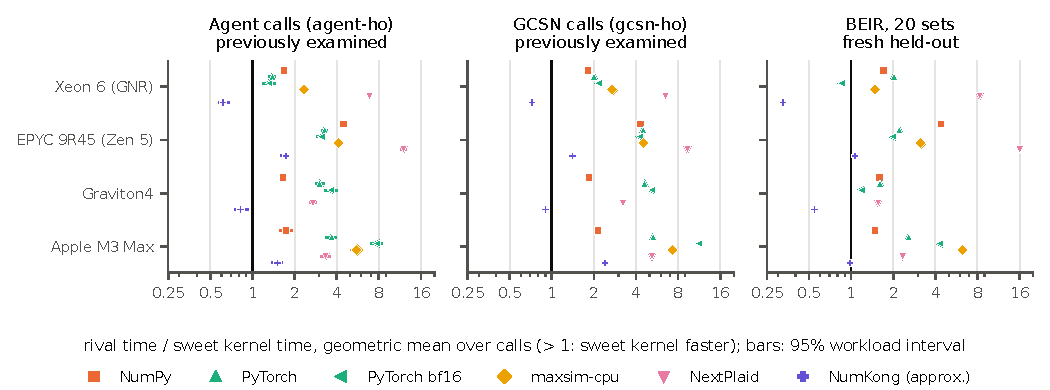
\includegraphics[width=\linewidth]{figures/ratios.pdf}
\caption{Warm speed ratios, all cores (rival time / \sweet time; above 1: \sweet faster), with the 95\% workload interval. Frozen rival configurations; NumKong shows its fastest input type. Agent and GCSN calls are previously examined; BEIR is fresh held-out.}
\label{fig:ratios}
\end{figure}

\subsection{Size sweep}
\label{sec:sweep}

Figure~\ref{fig:sweep} shows, per sweep cell, the fastest frozen exact float32 rival against \sweet.
On the cloud CPUs all 84 cells ran; the M3 Max ran \nm{sweep.m3max.cells} cells (a reduced grid of 24, decided before any result, plus 2 complete cells from before that decision).
The fastest exact rival was faster than \sweet in \nm{sweep.intel.lose} of \nm{sweep.intel.cells} cells on Intel, \nm{sweep.amd.lose} on AMD, \nm{sweep.arm.lose} on Graviton4 and \nm{sweep.m3max.lose} of \nm{sweep.m3max.cells} on the M3 Max.
The losses form bands.
On AMD, PyTorch was faster for pools of 64 to 1,024 short documents at every query length (worst cell: \nm{sweep.amd.worstcell}, \nm{sweep.amd.worst}$\times$), while \sweet was faster for smaller and larger pools.
On Intel and Graviton4, most losses are at 32 and 64 query tokens with 64 to 4,096 documents (mostly PyTorch, some NextPlaid), plus single documents with 32 or 64 query tokens (NumPy).
On the M3 Max, maxsim-cpu and PyTorch (both on Apple Accelerate, which uses the AMX matrix unit) were faster for single documents with 32 or 64 query tokens and for the largest pools.
At 8 query tokens, \sweet was faster in every cell on Intel, Graviton4 and the M3 Max.
We did not decompose the cost of a call (Section~\ref{sec:limits}), so these figures show where \sweet loses, not why.
NumKong is not in the figure; it was faster than \sweet in most sweep cells on every CPU (Section~\ref{sec:losses}).

\begin{figure}[!htbp]
\centering
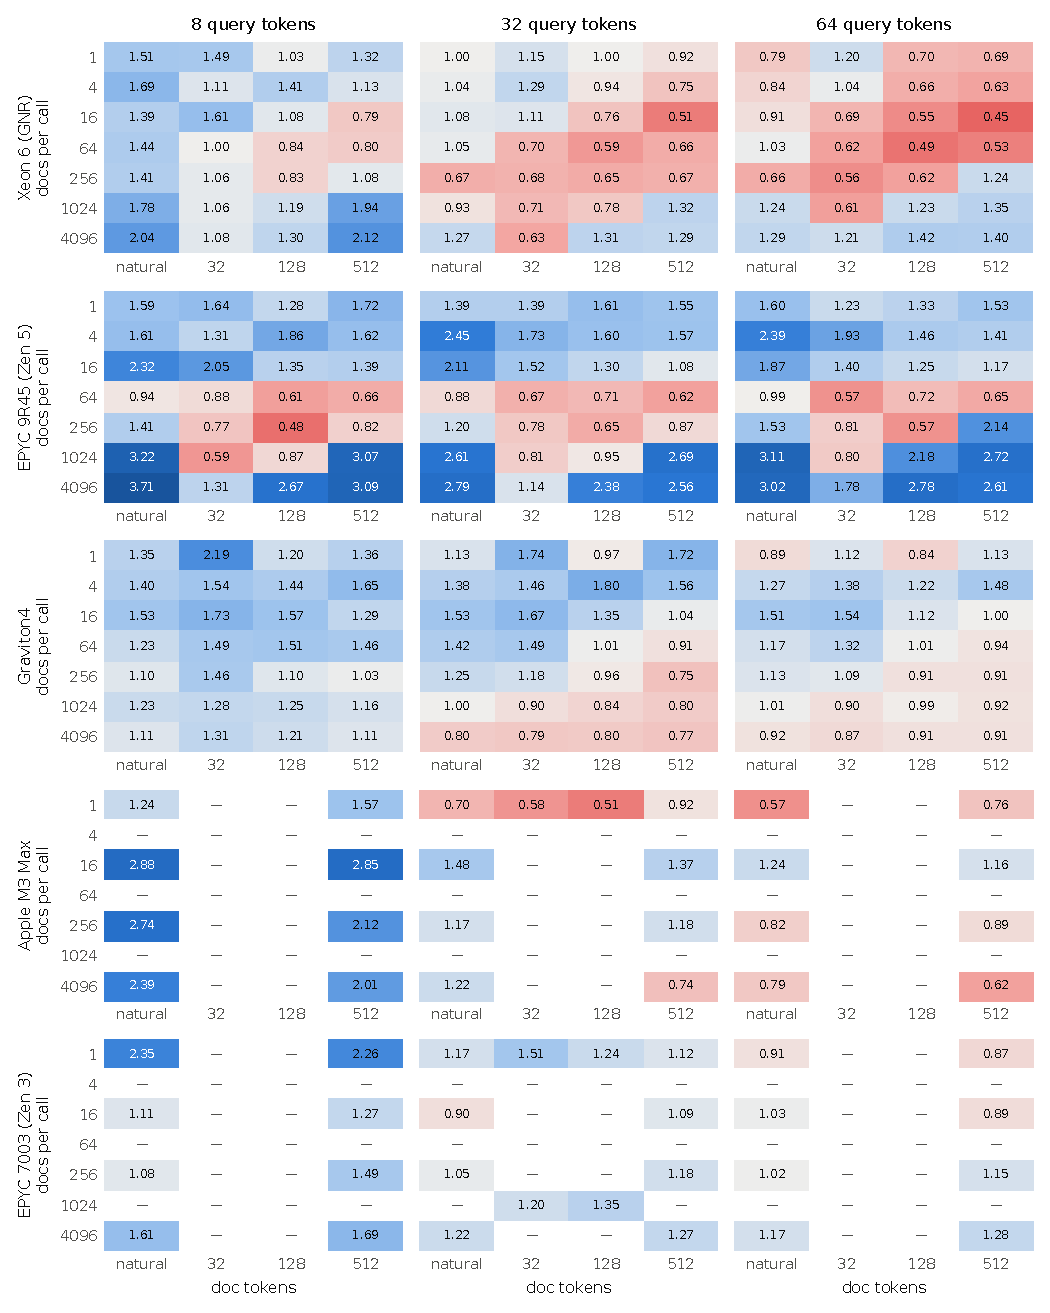
\includegraphics[width=\linewidth]{figures/sweep.pdf}
\caption{Size sweep (previously examined), warm, all cores: fastest frozen exact float32 rival / \sweet per cell (geometric mean over the cell's calls; blue: \sweet faster, red: the rival is faster; log colour scale). Rows: CPUs; columns: query tokens; inside: documents per call $\times$ tokens per document. ``--'': cell not run (reduced local grid).}
\label{fig:sweep}
\end{figure}

\subsection{Quality on BEIR: int4 against float32}
\label{sec:quality}

\paragraph{The pre-registered test.}
Before the freeze we fixed four primary comparisons (both models $\times$ both datasets, $k = 100$), the margin $\delta = 0.01$ absolute nDCG@10, and the decision rule.
For each set, ``no material loss'' holds only if on every CPU both the lower bound of the paired-bootstrap 95\% interval of (K $-$ F) is above $-\delta$ and the Holm-adjusted one-sided $p$ for $H_0$: loss $\geq \delta$ is below 0.05.
K is the kernel's own recorded scores; F scores the float32 vectors in float64 without clamp.
Table~\ref{tab:primary} gives the result.
For ColBERTv2, both sets pass on every CPU: K $-$ F is \nm{q.intel.scifact.colbertv2.diff} on SciFact and \nm{q.intel.nfcorpus.colbertv2.diff} on NFCorpus.
For answerai-colbert-small, both sets fail on every CPU: K $-$ F is \nm{q.intel.scifact.answersmall.diff} (\nm{q.intel.scifact.answersmall.rel}\%) on SciFact and \nm{q.intel.nfcorpus.answersmall.diff} (\nm{q.intel.nfcorpus.answersmall.rel}\%) on NFCorpus.
The secondary contrast (Q+c $-$ F, int4 decoded in float64 under contract S) gives the same values, because K and Q+c give the same nDCG@10 to four decimals in every cell, on every CPU and every $k$.

\begin{table}[!htbp]
\centering\scriptsize
\setlength{\tabcolsep}{3pt}
\caption{Primary non-inferiority tests (fresh held-out; $k = 100$; $\delta = 0.01$ absolute nDCG@10; paired bootstrap over queries, 10,000 resamples, seed 42; Holm over the four tests). Per CPU: lower 95\% bound of K $-$ F / Holm-adjusted $p$, and the verdict (\cmark: no material loss).}
\label{tab:primary}
\resizebox{\linewidth}{!}{%
\begin{tabular}{llrrrrr|ccccc}
\toprule
dataset & model & queries & F & K & K $-$ F & relative & Intel & AMD & Graviton4 & M3 Max & EPYC \\
\midrule
\inputtable{tables/primary.tex}
\bottomrule
\end{tabular}}
\end{table}

\paragraph{Where the loss comes from.}
Table~\ref{tab:effects} separates the score sources at $k = 100$.
The clamp has no effect (F+c = F).
The kernel's arithmetic has no effect (K = Q+c).
The whole loss enters between F+c and Q+c, that is, with the int4 storage under contract S.
The decoding error itself is the same for both models: the median relative error of a decoded token is \nm{int4diag.scifact.colbertv2.relerr} for ColBERTv2 and \nm{int4diag.scifact.answersmall.relerr} for answerai-colbert-small, and the median cosine between a token and its decoding is \nm{int4diag.scifact.colbertv2.cos} and \nm{int4diag.scifact.answersmall.cos}.
The two models differ in what contract S does with that error.
Contract S divides the decoded token by the norm of the token \emph{before} quantization, so any change of length by quantization enters the score.
Contract C on the same int4 data divides by the norm of the decoded token itself; its nDCG@10 (C-b) is \nm{nd.scifact.answersmall.Cb} on SciFact and \nm{nd.nfcorpus.answersmall.Cb} on NFCorpus, close to the float32 values of \nm{nd.scifact.answersmall.F} and \nm{nd.nfcorpus.answersmall.F}.
This analysis is post hoc and descriptive: we did not pre-register it, and we did not change or test the production rule.
It suggests that the loss is a property of the normalization in the storage format, not of int4 precision as such and not of the kernel.

\begin{table}[!htbp]
\centering\scriptsize
\setlength{\tabcolsep}{3.5pt}
\caption{nDCG@10 by score source at $k = 100$ (fresh held-out). BM25: candidate order. F: float32 vectors, float64, no clamp; F+c: with clamp; Q+c: int4 decoded in float64, contract S; K: \sweet kernel scores; C-b: contract C on float64-decoded int4; C-a: contract C on NumKong's float32 inputs; NumKong: its recorded scores (float32 input, Intel run). Post-hoc columns: C-b, C-a.}
\label{tab:effects}
\begin{tabular}{llrrrrrrrr}
\toprule
dataset & model & BM25 & F & F+c & Q+c & K & C-b & C-a & NumKong \\
\midrule
\inputtable{tables/effects.tex}
\bottomrule
\end{tabular}
\end{table}

\paragraph{NumKong's approximation.}
Contract C itself costs little against S for ColBERTv2.
NumKong's token selection costs more: on SciFact with answerai-colbert-small, its own scores give nDCG@10 \nm{nd.scifact.answersmall.NK} against \nm{nd.scifact.answersmall.Ca} for the exact value of its contract on its own inputs.
On the BEIR sets its top-ranked document agreed with the contract-S reference on only 57--58\% of calls; its bfloat16 path on the Xeon, which uses AMX, agreed on 78\% (Table~\ref{tab:correctness}).

\paragraph{The kernel across CPUs.}
The kernel's BEIR scores were bit-identical between Intel and AMD (both AVX-512) and between Graviton4 and the M3 Max (both NEON).
Between the two instruction sets, \nm{xplat.armequal.lo}--\nm{xplat.armequal.hi}\% of scores were bit-identical and the largest difference was \nm{xplat.maxabs}; the full candidate ranking was the same on at least \nm{xplat.sameranking.min}\% of calls, and nDCG@10 agreed to four decimals.
Within one CPU, the scores of all thread budgets, rounds and processes were bit-identical (2,000 result files, 48 million scores).

\subsection{Quality per latency budget}
\label{sec:budget}

A faster scorer can rerank more candidates within the same time.
Figure~\ref{fig:budget} plots nDCG@10 against the per-request p95 of the timed scoring call, one point per $k$; Table~\ref{tab:budget} reads it at two budgets.
The time covers only the scoring call: the rivals' decoding and casting run outside their timer.
At a p95 budget of 0.25\,ms, \sweet reached $k = $ \nm{budget.intel.scifact.colbertv2.0.25.ours} (Intel), \nm{budget.amd.scifact.colbertv2.0.25.ours} (AMD), \nm{budget.arm.scifact.colbertv2.0.25.ours} (Graviton4) and \nm{budget.m3max.scifact.colbertv2.0.25.ours} (M3 Max) on SciFact with ColBERTv2.
More candidates do not always help: with ColBERTv2 on SciFact, nDCG@10 is highest at $k = 25$, and with answerai-colbert-small on NFCorpus under contract S it falls as $k$ grows.
NumKong reaches $k = 200$ within 0.25\,ms on the three cloud CPUs, at the quality cost shown above.

\begin{figure}[!htbp]
\centering
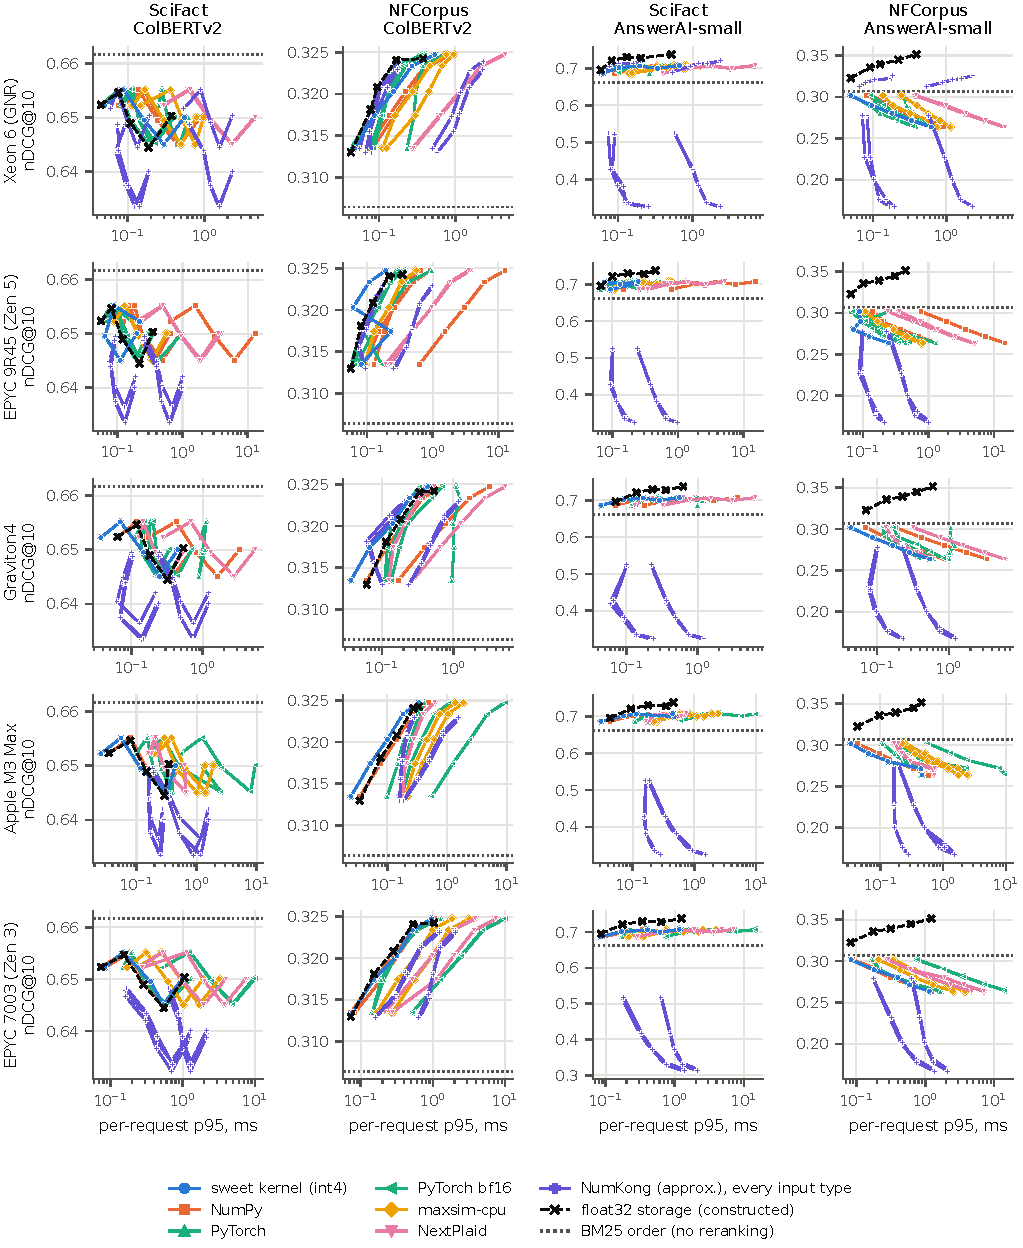
\includegraphics[width=\linewidth]{figures/budget.pdf}
\caption{Quality per latency budget (fresh held-out BEIR): nDCG@10 against per-request p95 of the timed scoring call, one point per $k \in \{10, 25, 50, 100, 200\}$. Frozen configurations; int4-self arms omitted (Table~\ref{tab:int4self}).}
\label{fig:budget}
\end{figure}

\begin{table}[!htbp]
\centering\scriptsize
\setlength{\tabcolsep}{3pt}
\caption{Largest $k$ whose per-request p95 fits the budget, with nDCG@10 at that $k$ in parentheses. ``best exact'': the frozen exact rival (any input type except int4-self) that reaches the largest $k$. NumKong: its best input type.}
\label{tab:budget}
\resizebox{\linewidth}{!}{%
\begin{tabular}{llllllll}
\toprule
& & \multicolumn{3}{c}{p95 $\leq$ 0.25\,ms} & \multicolumn{3}{c}{p95 $\leq$ 0.5\,ms} \\
CPU & set & \sweet & best exact & NumKong & \sweet & best exact & NumKong \\
\midrule
\inputtable{tables/budget.tex}
\bottomrule
\end{tabular}}
\end{table}

\subsection{Pool-parked calls (5\,ms busy gap)}
\label{sec:parked}

When other work runs for 5\,ms before each call, the worker pool of \sweet has parked and must be woken.
Table~\ref{tab:parked} shows that this changes the ranking.
NumPy was faster than \sweet on Intel (\nm{parked.intel.agent-ho.numpy.f32}$\times$ on agent calls, \nm{parked.intel.gcsn-ho.numpy.f32}$\times$ on GCSN calls, \nm{parked.intel.beir.numpy.f32}$\times$ on BEIR calls), on Graviton4 (\nm{parked.arm.agent-ho.numpy.f32}$\times$ and \nm{parked.arm.gcsn-ho.numpy.f32}$\times$) and on the M3 Max (\nm{parked.m3max.agent-ho.numpy.f32}$\times$ and \nm{parked.m3max.gcsn-ho.numpy.f32}$\times$). We did not measure why; one plausible cause is that OpenBLAS and Accelerate keep their threads awake longer than the 200\,$\mu$s spin of \sweet.
On AMD, \sweet stayed faster than every rival.
The product path calls a prewarm function when the rerank stage starts, so the pool wakes while other work runs; with it, a call took \nm{range.parked.prewarm.agent.min}--\nm{range.parked.prewarm.agent.max}$\times$ the time of the bare kernel (without prewarm) on agent calls.
On the Mac and the EPYC box, the BEIR idle-gap groups were not run (Appendix~\ref{app:deviations}).

\begin{table}[!htbp]
\centering\scriptsize
\setlength{\tabcolsep}{3pt}
\caption{Pool-parked calls (5\,ms busy gap before each call; 3 timed repetitions). Ratio = rival / \sweet kernel, both after the gap. ``prewarm'': the product path with its prewarm call; ``prod.\ path'': without it. BEIR: the 8 sets with $k \in \{25, 100\}$ (cloud CPUs only). Agent and GCSN previously examined; BEIR fresh.}
\label{tab:parked}
\begin{tabular}{llrrrrrrrrr}
\toprule
CPU & set & calls & NumPy & PyTorch & PyTorch bf16 & maxsim-cpu & NextPlaid & NumKong$^\dagger$ & prewarm & prod.\ path \\
\midrule
\inputtable{tables/parked.tex}
\bottomrule
\end{tabular}
\end{table}

\subsection{One thread}
\label{sec:single}

Table~\ref{tab:single} compares each library's frozen one-thread configuration with \sweet on one thread.
On agent and GCSN calls on the three Linux CPUs, \sweet was faster than every exact rival (the closest, NumPy, needed \nm{range.single.numpy.linux.agentgcsn.min}--\nm{range.single.numpy.linux.agentgcsn.max}$\times$ the time).
On BEIR calls (32-token queries, up to 200 candidates), a rival was faster on every CPU: NumPy on Intel (\nm{single.intel.beir.numpy.f32}$\times$) and AMD (\nm{single.amd.beir.numpy.f32}$\times$), PyTorch on Graviton4 (\nm{single.arm.beir.torch.f32}$\times$).
So the all-core advantage on BEIR calls does not come from faster arithmetic per core.
On the M3 Max, NumPy, PyTorch and maxsim-cpu call Apple Accelerate, which runs matrix products on the AMX coprocessor whatever the thread limit; their one-thread rows are therefore not one core against one core, and they were faster than \sweet on all three workloads.

\begin{table}[!htbp]
\centering\scriptsize
\setlength{\tabcolsep}{3pt}
\caption{One thread each (frozen one-thread configurations; not pinned to a core). Ratio = rival / \sweet with one thread. On the M3 Max, Accelerate-based rivals use the AMX coprocessor whatever the thread limit.}
\label{tab:single}
\begin{tabular}{llrrrrrrr}
\toprule
CPU & set & calls & NumPy & PyTorch & PyTorch bf16 & maxsim-cpu & NextPlaid & NumKong$^\dagger$ \\
\midrule
\inputtable{tables/single.tex}
\bottomrule
\end{tabular}
\end{table}

\subsection{Rivals on the same int4 storage}

When NumPy and maxsim-cpu receive the same int4 storage as \sweet and decode it inside their timed call, they were \nm{range.int4self.min}--\nm{range.int4self.max}$\times$ slower (Table~\ref{tab:int4self}).
This is the cost that the other rows leave out of the timer: in a system that stores int4, a float32 rival must decode before it scores, or keep a float32 copy (Section~\ref{sec:memory}).

\begin{table}[!htbp]
\centering\scriptsize
\caption{Rivals given the same int4 storage, decoding inside their timed call (``int4-self''). Ratio = rival / \sweet kernel, warm, all cores.}
\label{tab:int4self}
\begin{tabular}{llrr}
\toprule
CPU & set & NumPy int4-self & maxsim-cpu int4-self \\
\midrule
\inputtable{tables/int4self.tex}
\bottomrule
\end{tabular}
\end{table}

\subsection{Parallel callers}
\label{sec:conc}

In a service, several requests can score at the same time.
We ran $N \in \{1, 4, 16\}$ callers in two executors: threads in one process (the library's pool is shared), and one process per caller with a thread budget of $\max(1, \text{cores}/N)$.
\emph{Closed-loop saturation} lets each caller replay its share of a set back to back; we report throughput.
\emph{Open-loop} runs use one Poisson arrival trace per rate (seed 42; the same timestamps and call order for every arm); the rates are absolute and common to all arms on a machine: 25, 50 and 75\% of the closed-loop throughput of the slowest shortlisted rival on development data, frozen.
Their latency includes queueing.

Table~\ref{tab:conc} and Figure~\ref{fig:conc} give the results (best executor per arm).
With one caller, \sweet had \nm{range.conc.n1.min}--\nm{range.conc.n1.max}$\times$ the throughput of the best exact rival.
With 16 callers the margin shrank, and an exact rival had the higher throughput in two of eight CPU--workload pairs: NextPlaid on Graviton4 GCSN calls and NumPy on M3 Max agent calls.
NumKong had a higher throughput than \sweet at 16 callers in every pair.
At the highest common open-loop rate, the best exact rival had a lower per-request p99 than \sweet on M3 Max GCSN calls only.
During the analysis we found a defect in the harness: in closed-loop runs of the per-process executor, callers start about 50\,ms before the recorded start time, so the recorded wall time is too short.
We corrected these throughputs by adding 48.8--50\,ms (the bound follows from the 1\,ms polling of the start file) and report the lower bound; the per-request latencies need no correction (Appendix~\ref{app:deviations}).

\begin{table}[!htbp]
\centering\scriptsize
\setlength{\tabcolsep}{3pt}
\caption{Parallel callers (previously examined sets). Closed loop: \sweet throughput in thousand calls/s, and \sweet / best exact rival and \sweet / best NumKong configuration (above 1: \sweet faster; red: rival faster). Open loop: per-request p99 in ms at the highest common rate (calls/s), \sweet and the best exact rival (red: rival lower).}
\label{tab:conc}
\resizebox{\linewidth}{!}{%
\begin{tabular}{llrlrrlrrrl}
\toprule
& & \multicolumn{3}{c}{1 caller} & \multicolumn{3}{c}{16 callers} & \multicolumn{3}{c}{open loop, top rate} \\
CPU & set & \sweet & exact & NumKong & \sweet & exact & NumKong & rate & \sweet p99 & exact p99 \\
\midrule
\inputtable{tables/conc.tex}
\bottomrule
\end{tabular}}
\end{table}

\begin{figure}[!htbp]
\centering
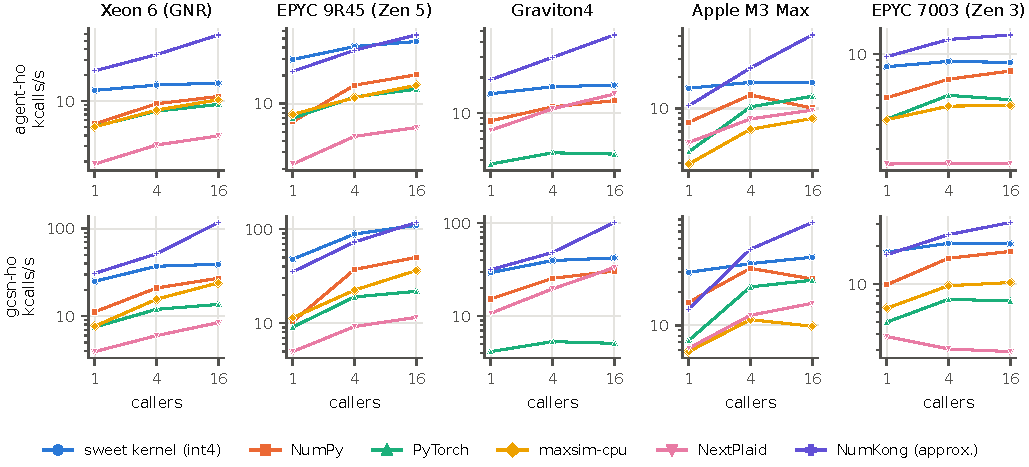
\includegraphics[width=\linewidth]{figures/conc.pdf}
\caption{Closed-loop saturation throughput against the number of callers (best executor per library; previously examined sets; log scales).}
\label{fig:conc}
\end{figure}

\subsection{Memory}
\label{sec:memory}

A separate, untimed pass per arm and set measured resident memory in a fresh process (Linux: \texttt{VmRSS}, \texttt{VmHWM} and \texttt{smaps\_rollup}; macOS: resident size from a 0.2\,ms sampler).
The allocator returned freed large blocks at once, so a later phase cannot reuse them unseen.
Table~\ref{tab:memory} reports resident bytes per stored document token (the int4 store for arms that read it, plus the arm's own prepared copy) and the peak temporary memory of the largest call.
\sweet holds \nm{mem.intel.ours.bpt} bytes per token at dimension 128 and \nm{mem.intel.ours.bpt96} at dimension 96, the size of the int4 store itself.
The float32 rivals hold their decoded copy: about 520 bytes per token for NumPy and \nm{mem.intel.torch_pad_bmm.bpt} for padded PyTorch on Intel.
The int4-self rivals hold the store and peak at about 280\,MB of temporary memory on the largest agent call.

\begin{table}[!htbp]
\centering\scriptsize
\caption{Memory on agent-ho (previously examined): resident bytes per stored document token / peak temporary memory of the largest call in MiB. Computed sizes at dimension 128: int4 76, bfloat16 256, float32 512 bytes per token.}
\label{tab:memory}
\begin{tabular}{lrrrrr}
\toprule
arm & Intel & AMD & Graviton4 & M3 Max & EPYC \\
\midrule
\inputtable{tables/memory.tex}
\bottomrule
\end{tabular}
\end{table}

\subsection{Instance-to-instance spread}
\label{sec:spread}

A replica instance of each cloud type repeated agent-ho and gcsn-ho.
Across \nm{replica.n} rival ratios, the ratio on the replica differed from the shard by a median of \nm{replica.median}\% and at most \nm{replica.maxabs}\%; no ratio changed sides of 1 (Table~\ref{tab:replica}).
The kernel's own geometric-mean latency differed by at most \nm{replica.oursmax}\%.
Each replica was a different instance in the same availability zone.
EC2 does not expose the physical host of shared-tenancy instances, so we cannot show that the hosts differed.

\begin{table}[!htbp]
\centering\scriptsize
\caption{Instance-to-instance spread: absolute relative difference of each frozen rival ratio between the shard and the replica instance (median and maximum, \%), and the change of the \sweet kernel's geometric-mean latency.}
\label{tab:replica}
\begin{tabular}{llrrrr}
\toprule
CPU & set & ratios & median \% & max \% & \sweet latency \% \\
\midrule
\inputtable{tables/replica.tex}
\bottomrule
\end{tabular}
\end{table}

\section{Where \sweet loses}
\label{sec:losses}

We list every case in which a frozen rival configuration was faster than \sweet.
Across all CPUs, modes, sets, sweep cells and frozen configurations, there are \nm{losses.total} such cases; Table~\ref{tab:losses} groups them, and the released analysis tables list each one.
``Significant'' counts the cases whose whole 95\% workload interval is below 1.

\begin{enumerate}
\item \textbf{NumKong, approximate.} With all cores and warm calls, NumKong was faster on Intel and Graviton4 on all three replayed workloads, about equal on M3 Max BEIR calls, and faster in most sweep cells on every CPU. It approximates the maximum (Section~\ref{sec:contracts}): on agent calls its top document agreed with the exact one on 86\% of calls, on BEIR calls on 57--58\%, and its BEIR quality fell sharply for answerai-colbert-small (Table~\ref{tab:effects}). It is a different trade-off, not an exact rival, but it is faster.
\item \textbf{bfloat16 on AMX.} PyTorch with bfloat16 inputs was faster on Intel BEIR calls (\nm{warm.intel.beir.torch.bf16}$\times$) and in many Intel sweep cells. It rounds its inputs to bfloat16; its top document agreed with the exact one on 97.5\% of BEIR calls and on 99.6--100\% of agent and GCSN calls.
\item \textbf{Mid-size and large sweep cells.} The fastest exact float32 rival beat \sweet in \nm{sweep.intel.lose} (Intel), \nm{sweep.amd.lose} (AMD), \nm{sweep.arm.lose} (Graviton4) and \nm{sweep.m3max.lose} (M3 Max) sweep cells; the lowest cell ratio was \nm{sweep.amd.worst} on AMD (Section~\ref{sec:sweep}). On AMD, the band of pools of 64 to 1,024 documents also covers sizes that occur in real calls (Table~\ref{tab:workload}).
\item \textbf{After an idle gap.} After 5\,ms of other work, NumPy was faster than the bare kernel on Intel, Graviton4 and the M3 Max on agent and GCSN calls, and on Intel BEIR calls (Section~\ref{sec:parked}). With the product path's prewarm call, \sweet was about as fast as NumPy on Intel agent calls (\nm{parked.intel.agent-ho.node-prewarm} against \nm{parked.intel.agent-ho.numpy.f32}) and faster on M3 Max agent calls, but still slower on Graviton4 (\nm{parked.arm.agent-ho.node-prewarm} against \nm{parked.arm.agent-ho.numpy.f32}).
\item \textbf{One thread.} With one thread, a rival was faster on BEIR calls on every CPU, and on the M3 Max on every workload (Section~\ref{sec:single}).
\item \textbf{Parallel callers.} At 16 callers, NumPy (M3 Max, agent calls) and NextPlaid (Graviton4, GCSN calls) had a higher throughput than \sweet, and NumKong had a higher throughput everywhere. At the highest common open-loop rate, NumPy had a lower p99 latency on M3 Max GCSN calls (Section~\ref{sec:conc}).
\item \textbf{Quality with one model.} Contract S on int4 storage lost \nm{q.intel.scifact.answersmall.relabs}\% and \nm{q.intel.nfcorpus.answersmall.relabs}\% nDCG@10 for answerai-colbert-small (Section~\ref{sec:quality}). Every float32 rival on the same int4 data inherits the same loss, but a system that stores float32 does not have it.
\end{enumerate}

\begin{table}[!htbp]
\centering\scriptsize
\caption{Cases where a frozen rival configuration was faster than \sweet, by CPU and mode. Count (in parentheses: whole 95\% interval below 1), libraries involved, and the worst ratio with its set or sweep cell (q = query tokens, d = documents, len = doc tokens).}
\label{tab:losses}
\begin{tabular}{lllrll}
\toprule
CPU & mode & rival & cases & libraries & worst ratio (where) \\
\midrule
\inputtable{tables/losses.tex}
\bottomrule
\end{tabular}
\end{table}

\section{Correctness findings}
\label{sec:correctness}

Every arm was checked on every call against a float64 reference of its own contract.
Table~\ref{tab:correctness} (Appendix~\ref{app:tables}) lists, per CPU and arm, the largest implementation error, the input-rounding effect and the top-1 agreement with the contract-S reference.
Apart from maxsim-cpu on the M3 Max (issue \#5 below), every exact arm with float32 inputs stayed within $4\times10^{-7}$ of its own reference on every call.
The checks found two new defects in other libraries and confirmed a third that was already reported. We reported the two new ones upstream in October 2026. The NumKong maintainer acknowledged the AMX defect, and another contributor opened a fix~\cite{numkong_pr409}; the maxsim-cpu report is still open.

\paragraph{maxsim-cpu, x86 build, long queries (issue \#1).}
For queries with more than 32 tokens, once a document has 64 or more tokens, the x86 wheel of maxsim-cpu~0.1.0 returned wrong scores, up to $10^{38}$ and infinity.
Another user had reported this behaviour in 2025~\cite{maxsimcpu_issue1}; our reference check found it independently, and we reproduced it on a second x86 CPU.
Its sums over 32-token query chunks are exact, so the benchmark calls it that way on x86; fewer than 1\% of agent calls have more than 32 query tokens.

\paragraph{maxsim-cpu, AArch64 build, zero padding (issue \#5).}
Its list interface pads shorter documents with zero vectors inside a call.
A zero vector scores 0, so for a query token whose best cosine is negative, the padded documents get 0 instead: a $\max(0,\cdot)$ clamp that depends on which other documents share the call~\cite{maxsimcpu_issue5}.
The ragged-length fixture catches it on AArch64.
On the M3 Max its largest error against its own contract was $4\times10^{-2}$ to $8\times10^{-2}$; its top document still agreed with the contract-S reference on every call, because S applies the same clamp on purpose.

\paragraph{NumKong, AMX path (issue \#406).}
On CPUs with AMX, NumKong~7.8.5's packed MaxSim kernel scans all 16 columns of a partially filled last tile.
When a document's token count modulo 64 is 49 to 63 and every cosine of a query token is negative, a padding column wins, and the result is wrong (NaN, 0, 1 or very large values)~\cite{numkong_issue406}.
The negative-best-match fixture found it on the Granite Rapids machine, and a standalone script reproduced it on a second machine of the same type.
The defect also occurred on the replayed data. On Intel, NumKong's float16 arms returned NaN scores on \nm{nan.intel.numkong_native_f16.ho-warm.agent-ho}\% of agent calls, \nm{nan.intel.numkong_native_f16.ho-warm.gcsn-ho}\% of GCSN calls and \nm{nan.intel.numkong_native_f16.ho-warm.beir}\% of BEIR calls; its float32 arms did so on up to \nm{nan.intel.numkong_native_f32.ho-warm.sweep}\% of sweep calls. No arm returned NaN on the CPUs without AMX. The defect's other wrong values (0, 1, very large) are not NaN and can hide inside NumKong's approximation error, so the Intel NumKong rows include an unknown number of further defective calls. Across runs, NumKong's Python arms on Intel also returned different scores for the same call (values up to $10^{74}$), while every other arm on every CPU returned bit-identical scores in all its runs. Their timings stand as measured and are marked ($\ast$) in the speed tables; their error and quality numbers do not describe NumKong's intended behaviour, so we take NumKong's quality from the AMD run.

\paragraph{Contract differences are not defects.}
NumKong's cosine of the received vectors (contract C) and PyLate's zero-padding rule (contract S-pre-pad0) are design choices, not bugs. maxsim-cpu's zero padding counts as a defect because the same call gives different scores on its x86 and AArch64 builds and depends on the other documents in the call.
Table~\ref{tab:contract-effects} measures them reference against reference.
Contract C keeps the top document of contract S on \nm{ce.agent-ho.S-vs-C.top1}\% of agent calls and \nm{ce.gcsn-ho.S-vs-C.top1}\% of GCSN calls, but on only \nm{ce.beir.S-vs-C.top1}\% of BEIR calls.
The clamp changes the top document on at most 0.1\% of calls; the epsilon placement changes no score by more than $10^{-15}$.
So almost all of the S--C difference comes from normalization.
Both models produce token vectors of unit length, so the stored norm $n_j$ is 1 (Section~\ref{sec:contracts}).
On the float vectors, S and C therefore differ only by the epsilon and the clamp.
On int4 tokens, C divides by the decoded norm, and S does not.
On development data, the decoded norm differed from 1 by up to about 2.5\%.
The two rules diverge most on BEIR, where candidate scores lie closest together.

\begin{table}[!htbp]
\centering\scriptsize
\caption{Contract effects, float64 reference against float64 reference (held-out sets; calls with at least two candidates). No implementation error enters these numbers.}
\label{tab:contract-effects}
\begin{tabular}{llrrrr}
\toprule
set & effect & calls & max $|\Delta|$ & top-1 agreement & top-10 overlap \\
\midrule
\inputtable{tables/contract_effects.tex}
\bottomrule
\end{tabular}
\end{table}

\section{Share of MaxSim in a search}
\label{sec:pipeline}

Microseconds in the kernel matter only if MaxSim is a visible part of a search.
We timed the stages of the production search path of sweet-search with per-stage timers, on the held-out agent queries, on the M3 Max, with the production configuration and a CPU query encoder.
This measurement ran after the freeze, on the frozen code, and changed no kernel code.
We report aggregates only.

\begin{table}[h]
\centering\small
\caption{Share of each stage in the time of one search (held-out agent queries, M3 Max; median and p90 over queries). \TODO{pipeline study: pipeline time-share results}}
\label{tab:pipeline}
\begin{tabular}{lrr}
\toprule
stage & median share & p90 share \\
\midrule
query encoding & \TODO{pipeline} & \TODO{pipeline} \\
candidate fetch & \TODO{pipeline} & \TODO{pipeline} \\
int4 load & \TODO{pipeline} & \TODO{pipeline} \\
MaxSim & \TODO{pipeline} & \TODO{pipeline} \\
the rest & \TODO{pipeline} & \TODO{pipeline} \\
\bottomrule
\end{tabular}
\end{table}

\TODO{pipeline study: one paragraph on the result: which stage dominates; what share MaxSim takes; what a faster kernel can and cannot change. This is not an end-to-end speed-up claim.}

\section{Limits and what we did not do}
\label{sec:limits}

\paragraph{Scope.}
CPU only and reranking only.
We did not run GPU kernels, WARP, EMVB, PLAID's candidate generation or full engines; they solve a different problem (search over a corpus) or need a different input.
maxsim-lut uses a compressed residual format and therefore another contract; we discuss it but did not run it.

\paragraph{No cost decomposition.}
We froze a rule for a stronger claim before the held-out runs: ``use the stronger claim only if all hold: (a) at 14 query tokens, pool 25, 366 doc tokens per candidate, the fixed share $f/t$ of the fastest rival is $> 50\%$ on at least 4 of 5 CPUs; (b) the cost model predicts the measured winner on $\geq 80\%$ of held-out sweep cells; (c) it beats the constant-winner baseline by $\geq 10$ percentage points on held-out cells. Otherwise the narrow claim.''
The decomposition that this rule needs (stage variants of the kernel and a fitted cost model) was not built before the freeze, for lack of time.
The rule therefore could not apply, and the paper uses the narrow claim.
In particular, we do not know why \sweet loses in the sweep bands of Section~\ref{sec:sweep} or after an idle gap.

\paragraph{No historical progression study.}
A planned study of older kernel versions (optional in the frozen plan) was dropped for time.

\paragraph{Workloads.}
The agent and GCSN calls come from one engine with one production model (dimension 128).
Their shapes are unique calls with duplicates removed, not a request-frequency distribution.
The BEIR sets use two public models and two small datasets; FiQA was planned but not built, because its licence allows only non-commercial use and we could not release derived data.
Only the BEIR sets are fresh held-out data; the other sets were examined in an earlier version of this benchmark.

\paragraph{Machines.}
Three CPU types ran in a public cloud with shared tenancy, on four instances per type plus a replica instance; we measured the instance-to-instance spread but cannot show that the physical hosts differed.
The Mac and the EPYC box ran a reduced sweep grid (24 of 84 cells) and no BEIR idle-gap groups.
The Mac is a desktop computer; its idle gate allowed 15\% background load.
No arm was pinned to a core, and the one-thread runs are therefore one-thread, not one-core, results.

\paragraph{Interfaces.}
We measured each library through the tested interface (Python, or a Rust loop over its C API) with its best shortlisted configuration.
A different binding, BLAS build or batching scheme can change a rival's numbers.
Intel MKL NumPy did not install from Intel's index, and maxsim-cpu has no AArch64 Linux wheel.
The BLIS NumPy arms on AMD ran after the other arms of their groups, not interleaved with them.

\paragraph{Quality.}
The non-inferiority test covers $k = 100$ on four model--dataset pairs.
The normalization analysis of Section~\ref{sec:quality} is post hoc; we did not test a changed scoring rule.

\paragraph{Authors.}
The authors wrote \sweet and this benchmark.
The freeze, the frozen shortlist, the fixed claim rules and the release of all raw results are our answer to this conflict; readers can recompute every table.

\section{Reproducibility}
\label{sec:repro}

\paragraph{Code.}
The benchmark, the kernel and the analysis are in the public repository of sweet-search~\cite{sweetsearch_repo}, folder \texttt{eval/maxsim-bench}.
The frozen state is commit \texttt{a4317ba9}; the freeze file (\texttt{FREEZE.json}) holds the SHA-256 of every frozen file, the shortlists, $R$, $\delta$, the primary tests, the parallel-caller rates and the claim rule, and \texttt{freeze\_check.py} verifies them.
Lock files pin every Python and Rust dependency per platform.
The analysis code written after the freeze is in \texttt{paper/analysis}; one command per file rebuilds every table, figure and number of this paper (\texttt{paper/README.md}), and \texttt{RESULTS-paper.md} lists each number with its source file.

\paragraph{Data.}
The release \TODO{Zenodo DOI} holds every raw result file (each timed repetition of each call, scores for the BEIR sets, memory and parallel-caller records), the completeness logs, the replay sets whose licences allow it, and release identifiers with rebuild scripts for the others (Appendix~\ref{app:data}).
Cloud instance identifiers are replaced by neutral host labels; each scrubbed file carries its own SHA-256, and the job keys stored inside the files then no longer match a recomputed key.

\paragraph{Adding an implementation.}
An arm is a Python function that receives one call (query, candidates in the replay format) and returns one score per candidate, plus a contract name.
The harness times it, checks it against the reference of its contract and writes the same records as for every other arm.
A small example (one replay set, three arms) runs in under ten minutes on a laptop \TODO{reproduction example: path and timing}.


\bibliographystyle{plainurl}
\bibliography{refs,refs-own}

\appendix
\section{Deviations from the plan}
\label{app:deviations}

Every deviation from the frozen plan and every fix during the analysis, in one line each.
None changed a frozen file after the held-out runs began, except where stated.

\begin{small}
\begin{longtable}{rp{0.88\linewidth}}
\toprule
\# & deviation \\
\midrule
\endhead
1 & Parallel-caller harness, out-of-memory fixes (two). Development run, 2026-10-15: each caller process held the whole set. Held-out run, 2026-10-16: the parent process cached decoded inputs of every call; fixed in place on every machine before any other machine reached a parallel-caller group, new SHA-256 in the freeze file (commit \texttt{daf54122}); the one affected group (Graviton4, agent calls) ran again in full. Memory only; timing code unchanged. \\
2 & AMD: the BLIS NumPy arms were missing at the start of the held-out runs (a machine-name test in the setup script) and were added in place; they ran after the other arms of their groups, not interleaved. \\
3 & Intel: MKL NumPy did not install from Intel's index and is left out. The development ``NumPy (MKL)'' arm had in fact used OpenBLAS (a mislabelled duplicate). \\
4 & Repetitions: $R = \max(5, \text{noise rule}) = 5$; an early plan with $R = 3$ was corrected before any held-out run. \\
5 & Mac and EPYC box: reduced sweep grid, 24 of 84 cells (decided before any held-out result was read). The Mac also holds 2 further complete cells, reported; 6 cells started before the decision have no job list and are left out. \\
6 & Mac and EPYC box: all 8 BEIR idle-gap groups dropped for machine time (decided 2026-10-17 before any held-out result was read). BEIR idle-gap results come from the three cloud CPUs. \\
7 & gcsn-ho: 6 query texts (7 calls) that also occur in gcsn-dev were removed before the freeze. \\
8 & maxsim-cpu has no Linux AArch64 wheel: missing on Graviton4. \\
9 & maxsim-cpu issue \#5 (zero padding) is caught by the padding fixture on AArch64; recorded as a known upstream defect, not a pass. \\
10 & Kernel tuning (the AVX-512 block) used development data only, with a 3\% rule above the noise band and a bit-identity gate. The development runs used the kernel before this change. \\
11 & The GenCodeSearchNet index of the engine was rebuilt from the paper commit (the old index had lost a file); the development MRR@10 gate passed (86.74\% with the old and the new addon, all 3,600 queries). \\
12 & Mac: idle gate raised from 10\% to 15\% CPU use (desktop background load), logged. \\
13 & The Intel replica failed once (two fixture checks raced after a double restart) and was relaunched; the AMD replica was relaunched for the BLIS fix. \\
14 & Analysis fix: the per-machine summaries written during the runs did not use the frozen shortlist (a file-name mismatch); every table here was regenerated with it. \\
15 & Three commits define the freeze: \texttt{a4317ba9} (frozen code), \texttt{ea84951f} (freeze file re-made after a replica naming fix), \texttt{daf54122} (item 1). \TODO{post-freeze change: the machine-name test in the setup script, with old and new SHA-256; no result affected}. \\
16 & Analysis fix: the frozen quality script keys an implementation by the arm name inside the result file, which drops the thread budget and the BLIS variant. Its quality numbers are unaffected for the kernel (all kernel result files of a set are bit-identical), but its latency points pool several configurations; the quality-per-budget analysis here recomputes them per result file. \\
17 & Analysis fix: in closed-loop runs of the per-process parallel-caller executor, callers start up to 50\,ms before the recorded start; throughputs are corrected by 48.8--50\,ms (lower bound reported). Latencies need no correction. \\
18 & The cloud instance metadata does not expose the physical host of shared-tenancy instances; the replica is shown to be a different instance in the same zone, not a different host. \\
19 & The one-thread runs were not pinned to a core (the plan asked for pinning). \\
20 & EPYC box: \TODO{epyc: completeness and any group that ran despite the cut}. \\
\bottomrule
\end{longtable}
\end{small}

\section{Data and licences}
\label{app:data}

\begin{itemize}
\item \textbf{Agent sets}: embeddings of code chunks from 11 repositories under MIT or Apache-2.0 (composer, dgraph, drogon, GRDB.swift, jj, Ocelot, okhttp, sequel, tortoise-orm, typedoc, zipkin) and of agent queries. Released under CC-BY-4.0 with an attribution file. Query texts are not released (they may quote code).
\item \textbf{SciFact}: corpus ODC-By 1.0, claims CC-BY-4.0; embeddings, BM25 lists and identifiers released with attribution.
\item \textbf{NFCorpus}: ``free to use for academic purposes''; no redistribution statement. Released as identifiers, BM25 lists and the rebuild script only.
\item \textbf{GenCodeSearchNet}: CodeSearchNet functions carry per-repository licences that the dataset does not list. Released as identifiers and the rebuild script only.
\item \textbf{FiQA-2018}: non-commercial use only; not built.
\item \textbf{Models}: answerai-colbert-small-v1 (Apache-2.0) and ColBERTv2 (MIT); exact revisions are in the release manifest.
\end{itemize}

\section{Threats to validity and where we address them}
\label{app:threats}

An independent review of the plan raised the following points before any held-out run; the protocol answers each.

\begin{small}
\begin{longtable}{p{0.45\linewidth}p{0.48\linewidth}}
\toprule
concern & answer \\
\midrule
\endhead
Rivals compute different scores (normalization, epsilon, clamp, precision) & Four contracts, two float64 references per rival, contract effects measured apart (Section~\ref{sec:contracts}, Table~\ref{tab:contract-effects}) \\
Results seen before development ended; checks after held-out & One freeze before held-out runs; BEIR fresh; other sets labelled previously examined (Section~\ref{sec:freeze}) \\
Stale or skipped results; failures reported as done; unpinned dependencies & Job keys over set, arm, binary, options and instance; completeness check before any table; failure tests; lock files \\
Speed does not show that fixed costs dominate & Narrow claim; frozen claim rule not applicable without a decomposition (Section~\ref{sec:limits}) \\
Missing rivals; per-document Python calls & NextPlaid added; NumKong and NextPlaid looped natively; maxsim-lut discussed \\
Two rounds cannot resolve small effects; no provenance; configuration chosen on reported calls & $R = 5$ processes $\times$ 2 rounds, noise band per machine, provenance per call, frozen shortlist from development data \\
No quality margin; effects mixed; p50 is not a deadline & $\delta$ fixed before the freeze, effects separated, per-request p95/p99 from every timing \\
A version-by-version study cannot attribute speed & Not run; no attribution claimed \\
Physical cores on c8a; ``bytes read'' not measured; 8$\times$ storage claim & Cores and threads per machine; ``storage bytes''; $6.7\times$ \\
Unique calls; overlap between splits; ``cold'' naming; closed loop is not service latency & Stated in Section~\ref{sec:workload}; overlap removed; ``pool-parked''; open-loop runs at common rates \\
Contract C clamp, epsilon and precision unclear & Defined from NumKong's source (Table~\ref{tab:contracts}) \\
No independent fixtures & Hand-built fixtures with plain-Python expected values \\
Wake-up probe and ``unexplained remainder'' & Decomposition not run \\
No constant-winner baseline for a cost model & Part of the frozen claim rule; not reached \\
p95 of per-call medians is not a tail; per-arm rates are not equal traffic & Per-request percentiles; common absolute open-loop rates \\
Non-inferiority on the kernel's actual scores; $\delta$ absolute & K $-$ F primary, absolute $\delta$, relative loss shown \\
Validate on all five machines & Fixtures and development runs on all five machines before the freeze \\
Earlier sets stay previously examined on new CPUs & Labelled on every table \\
Failure handling untested & Harness failure tests (interrupted output, missing calls, failed arm, changed identity, resume) \\
Optional items must stay optional & Decomposition and version study not run, stated \\
\bottomrule
\end{longtable}
\end{small}

\section{Per-machine tables}
\label{app:tables}

\begin{small}
\setlength{\tabcolsep}{4pt}
\begin{longtable}{lllllrr}
\caption{Correctness per arm (warm; agent-ho previously examined, BEIR fresh): contract (+c: clamp), largest error against reference (a) of the arm's own contract, input-rounding effect, top-1 agreement with the contract-S reference.}\label{tab:correctness}\\
\toprule
CPU & set & arm & contract & max error & input rounding & top-1 = S \\
\midrule
\endfirsthead
\toprule
CPU & set & arm & contract & max error & input rounding & top-1 = S \\
\midrule
\endhead
\inputtable{tables/correctness.tex}
\bottomrule
\end{longtable}
\end{small}

Full per-machine tables for every set, sweep cell, mode and configuration (including the post-hoc fastest configurations) are in the released analysis folder (\texttt{paper/analysis/tables/speed.md}, \texttt{memory.md}, \texttt{conc.md}, \texttt{budget.md}).


\end{document}
